\documentclass{mycourse}
\usepackage[all]{xy}
\usepackage{array}
%\usepackage[a4paper,left=1 cm,right= 1cm, top=1cm, bottom=2cm] {geometry}

% Für Text zwischen enumerate-items aber ohne Bezug zu einem bestimmten item.
\makeatletter
\newcommand{\interitemtext}[1]{%
\begin{list}{}
{\itemindent=0mm\labelsep=0mm
\labelwidth=0mm\leftmargin=0mm
\addtolength{\leftmargin}{-8mm}}
\item #1
\end{list}}
\makeatother

\ifthenelse{\isundefined{\psmallmatrix}}{
	\newenvironment{psmallmatrix}{\left(\begin{smallmatrix}}{\end{smallmatrix}\right)}
}{}

\newcommand{\dist}{\operatorname{dist}}
\newcommand{\Ran}{\operatorname{Ran}}
\newcommand{\h}{\hslash}
\newcommand{\Tr}{\operatorname{Tr}}
\newcommand{\slim}{\operatorname{s-lim}}
%\renewcommand{\eqref}[1]{\hyperref[#1]{(#1)}}

\usepackage{bbold}

\title{Mathematische Methoden der Quantenmechanik}
\author{}
\date{\today}

\begin{document}

\maketitle
\tableofcontents

\chapter*{Motivation und Inhaltsübersicht}
Die Aufgaben der Quantenmechanik kann man einteilen in
\begin{enumerate}[1)]
\item Dynamiken von Systemen zu bestimmen, gegeben durch die Schrödingergleichung $i\dot \psi=H\psi$, wobei $H$ der Hamiltonoperator (formal symmetrischer Operator der durch physikalische Literatur gegeben ist).
\item Wahrscheinlichkeit von Messergebnissen bestimmen. 
\end{enumerate}
Die Lösung der Schrödingergleichung ist gegeben durch
\[
\psi_t = e^{-i \tilde H t} \psi_0,
\]
wobei $\tilde H$ eine selbstadjungierte Erweiterung von $H$ ist (vgl Satz \ref{3.9}) oder mit dem Funktionalkalkül (vgl. Kapitel \ref{6})
\[
e^{-i \tilde H t} = \Phi(e_t), e_t(\lambda) = e^{-i\lambda t}.
\]
$\tilde H=\overline{H}$ wenn $H$ wesentlich selbstadjungiert ist (vgl. Kapitel \ref{3}), dann ist $\tilde H = \overline H$ die einzige selbstadjungierte Erweiterung von $H$. Des brauchen wir Kriterien für Selbstadjungiertheit bzw. wesentlicher Selbstadjungiertheit (siehe Kapitel \ref{3} und Kapitel \ref{5}).

\emph{Nichtautonome Schrödingergleichungen}
\[
i \dot \psi = H(t) \psi
\] 
beschreiben Systeme die von zeitabhängigen äusseren Feldern abhängen (typisch im Experiment!). Die Existenz der Zeitrevolution sichert uns der Satz von Kato \ref{4.4}. Der Satz von Phillips \ref{4.3} gibt uns eine Kontruktion mittels Propagator als Dysan-Reihe. (vgl. zeitabhängige Störungstheorie).

Typischerweise ändert sich $H(t)$ sehr langsam im Vergleich zu quantenmechanischen Prozessen, was zum \emph{Adiabatische Theorem führt} (siehe Kapitel 4.2 oder Griffiths).

Observablen (beobachtbare Größen) werden in der Quantenmechanik beschrieben durch selbstadjungierte Operatoren. Die Wahrscheinlichkeit, dass bei einer Messung von der Größe beschrieben durch $A=A^*$ im Zustand $\phi$ ein Wert in $\Omega \subset \R$ gemessen wird ist
\[
\mu_\phi(\Omega) = \< \phi, P_\Omega \phi \>,
\]
wobei $P_\Omega$ das Spektralmaß von $A$ ist. Die Formel für $P_\Omega$ ($\Omega$ isoliert) ist dabei gegeben durch
\[
P_\Omega = \frac{1}{2\pi i} \oint_\gamma (z-A)^{-1} \, \dx[z] 
\]
(vgl auch Formel von Stone).

Ist $\lambda$ ein Eigenwert von $A$ mit $A\phi = \lambda \phi$, $\| \phi \|=1$, dann ist
\[
\mu_\phi(\{\lambda \}) = \< \phi, P_{\{\lambda\}} \phi \> = \< \phi, \phi \> =1.
\]
D.h. $\lambda$ wird mit Wahrscheinlichkeit $1$ gemessen. Also sind Eigenzustände, Zustände die man mit Sicherheit voraussagen kann.

Die Eigenwerte von $A= H_0 + \kappa V$ kann man mit Störungstheorie approximieren (siehe Kapitel 2, zeitunabhängige Störungstheorie in der Quantenmechanik).

Es gibt dabei einen Zusammenhang zwischen Dynamik und Spektrum, der sich durch
\begin{align*}
e^{-i Ht} \phi &= \int_{\sigma(H)} e^{-i\lambda t} \, \dx[P_\phi]\\
(z-H)^{-1}&= -i \int_0^{\pm \infty} e^{izt} e^{-iHt} \, \dx[t]
\end{align*}
(vgl. Streutheorie s. Vorlesungsskript).


Weiterführendes: (BCS-Theorie, wurde nicht behandelt).

\chapter{Lineare Operatoren}\label{1}
\section{Spektrum linearer Operatoren}
Sei $H$ ein Hilbertraum über $\C$ mit Skalarprodukt $\langle \cdot, \cdot \rangle$. Sei $D\subset H$ ein linearer Teilraum von $H$ und $A:D\to H$ ein linearer Operator. Dann ist $D=D(A)$ der \emph{Definitionsbereich} von $A$ und $AD=\{A\phi|\, \phi\in D\}$ heißt \emph{Wertebereich} (range) von $A$.

Die \emph{Resolventenmenge} $\rho(A)$ von $A$ ist definiert als 
\[
\rho(A)=\{z\in \C|\, z-A: D\to H \text{ bijektiv $(z-A)^{-1}$ ist beschränkt}\}.
\]

Die \emph{Resolvente} von $A$ ist die Abbildung $R=R_A: \rho(A) \to \mathcal L(H)$, gegeben durch $R(z)=(z-A)^{-1}$.

Das \emph{Spektrum} $\sigma(A)$ von $A$ ist definiert durch $\sigma(A)=\C\setminus \rho(A)$. Man zerlegt $\sigma(A)$ in
\begin{seg}[Punktsprektum]
Das \emph{Punktspektrum} ist gegeben durch
\[
\sigma_p(A)=\{z\in \C |\, (z-A): D\to H \text{ nicht injektiv}\}= \text{Menge der Eigenwerte.}
\]
\end{seg}
\begin{seg}[stetiges Spektrum]
Das \emph{kontinuierliche Spektrum} ist gegeben durch
\[
\sigma_c(A)=\{z\in \C|\, (z-A): D\to H \text{ injektiv, } \neg \text{ invertierbar aber } \overline{(z-A)D}= H\}.
\]
\end{seg}
\begin{seg}[Resdual-Spektrum]
Das \emph{Residual-Spektrum} oder auch \emph{Rest-Spektrum} ist gegeben durch
\[
\sigma_r(A)=\{z\in \C|\, (z-A):D \to H \text{ injektiv, aber } \overline{(z-A)D}\neq H\}.
\]
\end{seg}
\begin{nt*}
\begin{enumerate}[1)]
\item Falls $A$ abgeschlossen, d.h. wenn $\Gamma_A= \{(\phi, A\phi)|\, \phi \in D\}$ abgeschlossen ist in $H\times H$, und $z-A: D \to H$ bijektiv ist, dann ist $z-A$ und somit auch $(z-A)^{-1}$ abgeschlossen. Nach dem Graphensatz ist somit $(z-A)^{-1}$ beschränkt. D.h. wenn $A$ abgeschlossen ist, dann 
\[
\rho(A)=\{z\in \C|\, z-A: D \to H \text{ bijektiv}\}.
\]
Umgekehrt wenn $\rho(A)\neq \emptyset$, dann existiert $z\in \C$, so dass $(z-A):D\to H$ bijektiv und $(z-A)^{-1}$ beschränkt und somit abgeschlossen ist. Es folgt, dass $(z-A)$ und daher auch $A$ abgeschlossen ist.
\item wenn $A$ abgeschlossen ist, dann ist
\[
\sigma(A)=\sigma_p(A) \dot\cup \sigma_c(A) \dot\cup \sigma_r(A).
\]
\end{enumerate}
\end{nt*}
\begin{ex*}
\begin{enumerate}[1)]
\item Sei $H= l^2(\N_0)=\{(x_n)_{n=0}^\infty |\, x_n \in \C,\, \sum_{n=0}^\infty|x_n|^2<\infty\}$ und sei $A: H\to H$ gegeben durch 
\[
A(x_0, x_1, x_2,...)=(x_1, x_2,...).
\]
Dann ist $A\in \mathcal L(H)$ mit $\|A\|=1$
\[
\sigma_p(A)=\{z\in \C|\, |z|<1\}, \quad \sigma_c(A)=\{z\in \C|\, |z|=1\}, \quad \sigma_r(A)=\emptyset
\]
(Beweis: Übung).
\item $H=L^2(\R)$, $D=\{\phi\in L^2(\R)| \phi'\in L^2\}$ und $A\phi=-i \phi'$. Dann $\sigma(A)=\sigma_c(A)=\R$. Entsprechend folgt $\sigma_p(A)=\sigma_r(A)= \emptyset$. Beweis ist eine leichte Übung.
\end{enumerate}
\end{ex*}
Sind $A,B$ lineare Operatoren in $H$, dann heißt $B$ \emph{Erweiterung} von $A$ falls $D(A) \subset D(B)$ und $A\phi=B\phi$ für alle $\phi \in D(A)$. Der Operator $A$ \emph{vertauscht} mit $L\in \mathcal L(H)$, falls $LA\subset AL$, d.h. $LD(A)\subset D(A)$ und für alle $\phi \in D(A)$ gilt $LA\phi=AL\phi$.
\begin{st}\label{1.1}
Sei $A: D \subset H\to H$ ein linearer Operator mit Resolvente $R$. Dann gilt
\begin{enumerate}[a)]
\item $R(z)-R(w)=(w-z) R(z) R(w)$,
\item $R(z) R(w)=R(w) R(z)$,
\item $R(z) A\subset A R(z)=zR(z)-\mathbb{1}$
\end{enumerate}
für alle $z,w\in \rho(A)$.
\end{st}
\begin{proof}
siehe Satz 1.1 aus dem Skript.
\end{proof}
\begin{st} \label{1.2} Sei $A$ ein linearer Operator in $H$. Dann ist $\rho(A)$ offen, $\sigma(A)$ abgeschlossen und $R: \rho(A) \to \mathcal L(H)$ ist analytisch genauer: ist $z_0\in \rho(A)$, dann $B(z_0, \| R(z_0)\|^{-1}) \subset \rho(A)$ und in dieser Kreisscheibe gilt
\[
R(z)=\sum_{n=0}^\infty (-1)^n R(z_0)^{n+1} (z-z_0)^n.
\]
Es gilt außerdem $\|R(z_0)\|\ge \frac{1}{\dist(z_0, \sigma(A))}$.
\end{st}
\begin{proof}
siehe Satz 1.2 aus dem Skript.
\end{proof}
\begin{st}
Sei $A$ ein linearer Operator in $H$, $z_0\in \rho(A)$ und $L\in \mathcal L(H)$. Dann gilt 
\[
LR(z_0)=R(z_0)L \implies LA \subset AL \implies LR(z)=R(z)L
\]
für alle $z\in \rho(A)$.
\end{st}
\begin{proof}
siehe Satz 1.4 aus dem Skript.
\end{proof}

Sei $P\in \mathcal L(H)$ ein Projektor (d.h. $P^2=P$), dann ist auch $(I-P)$ ein Projektor und 
\[
H=M \oplus N,
\]
wobei $M=PH=\ker(I-P)$ und $N=(1-P)H=\ker(P)$. D.h. jeder Vektor $\phi\in H$ lässt sich eindeutig zerlegen in $\phi=\phi_1+\phi_2$ mit $\phi_1\in M$ und $\phi_2\in N$. Dabei gilt $\phi_1=P\phi$ und $\phi_2=(1-P)\phi$.

Ist $A$ ein linearer Operator in $H$ welcher mit den Projektoren $P$ vertauscht, also $PA\subset AP$. Dann wird $A$ durch $M=PH, N=(\mathbb{1}-P)H$ zerlegt in die beiden Operatoren
\[
A_P:=A \upharpoonright PH: PD(A) \to PH, \quad A_{\bar{P}}:=A \upharpoonright \bar PH: \bar P D(A) \to \bar{P}H,
\] 
wobei $\bar P:=\mathbb{1}-P$.
\begin{lem}\label{1.4}
Ist $A$ ein abgeschlossener linearer Operator in $H$ und $P\in \mathcal L(H)$ ein Projektor mit $PA \subset AP$. Dann gilt 
\[
\sigma(A)=\sigma(A_p)\dot\cup \sigma(A_{\bar{P}}).
\]
\end{lem}
\begin{proof}
Sei $z\in \C$. Dann ist $(z-A):D(A) \to H$ genau dann bijektiv, wenn $z-A_P: PD(A)\to PH$ und $z-A_{\bar{P}}:\bar P D(A) \to \bar P H$ bijektiv sind. Also $\rho(A)=\rho(A_p) \cap \rho(A_{\bar P})$ und somit $\sigma(A)=\sigma(A_P) \cup \sigma(A_{\bar P})$. Tatsächlich gilt
\[
(z-A_P)^{-1}=(z-A)^{-1} \upharpoonright PH, \quad (z-A_{\bar P})^{-1} = (z-A)^{-1} \upharpoonright \bar PH.
\]
\end{proof}
\section{Rieszprojektoren und Laurentreihe der Resolvente}
\subsection{Der Riesz-Projektor}
Sei $A$ ein abgeschlossener linearer Operator in $H$ und sei $\lambda\in \sigma(A)$ ein isolierter Punkt des Spektrums von $A$. D.h. es gibt ein $\eps>0$ so, dass $\overline{B_\eps(\lambda)} \cap \sigma(A)=\{\lambda\}$. Wir definieren den \emph{Riesz-Projektor} $P$ durch
\[
P:= \frac{1}{2\pi i} \oint_{|z-\lambda|=\eps} R(z) \, \dx[z],
\]
wobei das Integral als Riemannintegral aufgefasst ist.  
\begin{st}\label{1.5}
\begin{enumerate}[a)]
\item $P$ ist ein Projektor.
\item $PA\subset AP=\frac{1}{2\pi i} \oint zR(z)\, \dx[z] \in \mathcal L(H)$.
\item $\sigma(A_P)=\{\lambda\}$,\quad $\sigma(A_{\bar P})=\sigma(A) \setminus \{\lambda\}$.
\end{enumerate}
\end{st}
\begin{proof}
Siehe Satz 1.6 des Skripts. Man merke an, dass $\sigma(A)=\{\lambda\} \dot\cup (\sigma(A)\setminus\{\lambda\})$ in zwei abgeschlossene Teile zerfällt.
\end{proof}
\begin{nt*}
Satz \ref{1.5} lässt sich verallgemeinern. 

Falls $\sigma(A)$ in zwei disjunkte abgeschlossene Teile $\sigma_1$ und $\sigma_2$ zerfällt. D.h. $\sigma(A)=\sigma_1\cup \sigma_2$ mit $\sigma_1\cap \sigma_2=\emptyset$ und $\sigma_1, \sigma_2$ abgeschlossen, wobei $\sigma_1$ kompakt ist und $P\in \mathcal L(H)$ definiert wird durch
\[
P=\frac{1}{2\pi i} \oint_\gamma (z-A)^{-1} \, \dx[z],
\]
wobei die Windungszahl $n(\gamma, z)=1$ für $z\in \sigma_1$ und $n(\gamma,z)=0$ für $z\in \sigma_2$ und $\tr(\gamma)\subset \rho(A)$. Dann gilt
\begin{st}\label{1.6}
\begin{enumerate}[a)]
\item $P$ ist ein Projektor.
\item $PA\subset AP=\frac{1}{2\pi i} \oint zR(z)\, \dx[z] \in \mathcal L(H)$.
\item $\sigma(A_P)=\sigma_1$,\quad $\sigma(A_{\bar P})=\sigma_2$.
\end{enumerate}
\end{st}
\end{nt*}
\subsection{Laurentreihe der Resolventen}
Nach Satz \ref{1.5} gilt für $z\in B_\eps(\lambda)\setminus\{\lambda\}$
\[
(z-A)^{-1}=(z-A)^{-1}P+(z-A)^{-1}\bar P=(z-A_P)^{-1} P + (z- A_{\bar P})^{-1} \bar P,
\]
wobei $A_P$ und $A_{\bar P}$ die Einschränkungen von $A$ auf $PH$ bzw. $PH$ sind. Ausserdem ist $\sigma(A_p)=\{\lambda\}$, $\sigma(A_{\bar P}) \subset \sigma(A) \setminus\{\lambda\}$. Also gilt
\[
(z-A_P)^{-1} = \sum_{n\ge 0} \frac{(A_P-\lambda)^n}{(z-\lambda)^{n+1}}, \quad (z-A_{\bar P})^{-1} \stackrel{\ref{1.2}}=\sum_{n\ge 0}(-1)^n (\lambda-A_{\bar P})^{-n-1} (z-\lambda)^n
\]
für alle $z\in B_\eps(\lambda)\setminus\{\lambda\}$. Hierbei sei anzumerken, dass die Laurentreihenentwicklung konvergiert, da der Spektralradius von $(A_P-\lambda)$ gerade $0$ ist (Näheres siehe Appendix). Es folgt
\begin{st}
Für $0<|z-\lambda|<\eps$ gilt
\[
R(z)=\sum_{n=1}^\infty D^n(z-\lambda)^{-n-1} + \frac{P}{z-\lambda} + S(z), \quad S(z)=\sum_{n=0}^\infty (-1)^n S(\lambda)^n (z-\lambda)^n,
\]
wobei $D:=(A_P-\lambda)P=(A-\lambda)P$ und $S(z):= (z-A_{\bar P})^{-1}\bar P$ die reduzierte Resolvente ist.
\end{st}
\begin{nt*}
\begin{enumerate}[1)]
\item Da der Hauptteil von $R(z)$, d.h.
\[
\sum_{n=1}^\infty D^n(z-\lambda)^{-n-1} + \frac{P}{z-\lambda},
\]
konvergent ist für alle $z\neq \lambda$, gilt $\limsup_{n\to \infty} \|D^n\|^{1/n}=0$. Man sagt: $D$ ist \emph{quasi-nilpotent}.
\item Falls $D$ nilpotent ist, d.h. $D^m=0$ für ein $m\in N$ und $D^{m-1}\neq 0$, dann ist $\lambda$ ein Eigenwert von $A$. 
\begin{proof}
Wähle $\phi \neq 0$ mit $D^{m-1}\phi\neq0$. Dann ist $D(D^{m-1}\phi)=0$, d.h.
\[
(A-\lambda) (D^{m-1} \phi)=(A-\lambda) P(D^{m-1} \phi)= D^m \phi =0
\]
\end{proof}
\item Falls $m:= \dim(PH)<\infty$, dann ist $D^m=0$ und somit $\lambda$ ein Eigenwert von $A$. (Übung)

Dann heißt $\lambda$ ein \emph{diskreter Eigenwert} von $A$. Das Komplement der diskreten Eigenwerte innerhalb $\sigma(A)$ heißt \emph{wesentliches Spektrum} von $A$.
\end{enumerate}
\end{nt*}
\section{Der adjungierte Operator}
Sei $A:D\subset H\to H$ ein \emph{dicht definierter} linearer Operator, d.h. $\overline{D}=H$ (z.B. $D=H$). Der zu $A$ \emph{adjungierte Operator} $A^*: D(A^*)\subset H \to H$ ist wie folgt definiert. 

Wir sagen $\phi \in D(A^*)$ wenn $\phi^*\in H$ existiert, so dass $\langle \phi^*, \eta\rangle = \langle \phi, A\eta\rangle$ für alle $\eta \in D(A)$. Dann ist $\phi^*$ durch $\phi$ eindeutig bestimmt (da $\overline{D(A)}=H$) und man definiert $A^* \phi:= \phi^*$. Die Abbildung $\phi \mapsto A^*\phi$ ist linear. (Übung)

Nach Frechet-Riesz (genaueres siehe Übung) gilt
\[
D(A^*)=\{\phi\in H|\, \eta \mapsto \langle \phi, A\eta\rangle \text{ ist stetig auf } D(A)\}
\]

\begin{st}\label{1.8}
\begin{enumerate}[a)]
\item $A\subset B \implies A^*\supset B^*$.
\item $A^*$ ist abgeschlossen.
\item $\ker A^*=(R-A)^\orth$. 
\end{enumerate}
\end{st}
\begin{proof}
a) wurde in der Übung gezeigt. b) wird in Satz 2.1 aus dem Skript bewiesen. Und c) wird in Satz 2.2 aus dem Skript gezeigt.
\end{proof}
\begin{st}\label{1.9}
Ist A \emph{abgeschlossen}, dann ist $A^*$ dicht definiert und $(A^*)^*=A$.
\end{st}
\begin{proof}
Es ist
\begin{align*}
(\phi, \phi^*)\in \Gamma(A^*) &\iff \langle \phi^*, \eta\rangle = \langle \phi, A\eta\rangle, \, \forall \eta\in D(A)\\ &\iff 0=\langle \phi, A\eta\rangle - \langle \phi^*, \eta\rangle \\ &\iff (\phi, \phi^*) \orth (A\eta, - \eta)
\end{align*}
bezüglich des Skalarprodukts $\langle (\phi_1, \phi_2), (\psi_1, \psi_2)\rangle=\langle \phi_1, \psi_1\rangle + \langle \phi_2, \psi_2\rangle$ von $H\times H$. Sei $V:H\times H \to H \times H$ definiert durch $V(\phi, \psi)=(\psi, -\phi)$. Dann ist $V^2=\mathbb{1}$ und $V$ ist unitär. Für jeden Teilraum $E\subset H\times H$ gilt also $(VE)^\orth = V(E^\orth)$. (Übung)

Somit gilt
\begin{align*}
(\phi, \phi^*) \in \Gamma(A^*) &\iff (\phi, \phi^*) \orth V(\eta, A\eta), \, \forall \eta\in D(A)\\
&\iff (\phi, \phi^*)\in (V\Gamma(A))^\orth.
\end{align*}
D.h. 
\begin{equation}\label{eq:1.1}
\Gamma(A^*)=(V\Gamma(A))^\orth=V\Gamma(A)^\orth.
\end{equation}
Da $\Gamma(A)$ abgeschlossen ist folgt 
\begin{equation}\label{eq:1.2}
\Gamma(A) = ( \Gamma(A)^\perp)^\perp = (VV \Gamma(A)^\perp)^\perp - V(V\Gamma(A)^\perp)^\perp = V \Gamma(A^*)^\perp
\end{equation}
Wäre $D(A^*)$ nicht dicht, dann würde ein $\psi \neq 0$ existieren mit $\psi \perp D(A^*)$, d.h. $(\psi,0) \perp \Gamma(A^*)$, d.h. $(\psi,0) \in \Gamma(A^*)^\perp$ und 
\[
(0,-\psi)=V(\psi, 0) \in V \Gamma(A^*)^\perp= \Gamma(A). 
\]
Dies steht im Widerspruch zu $A0=0$. Also ist $D(A^*)$ dicht und
\[
\Gamma((A^*)^*)\stack{\eqref{eq:1.1}}= V \Gamma(A^*)^* \stack{\eqref{eq:1.2}}= \Gamma(A).
\]
Daraus folgt $(A^*)^*=A$.
\end{proof}
\begin{st}\label{1.10}
Ist $A$ dicht definiert und abgeschlossen, dann ist $z\in \rho(A)$ genau dann, wenn $\overline z \in \rho(A^*)$ und es gilt $(\overline z - A^*)^{-1} =((z-A)^{-1})^*$.
\end{st}
\begin{proof}
Wegen $(z-A)^* =(\overline z-A^*)$ und $(A^*)^*=A$ nach Satz \ref{1.2} genügt es zu zeigen, dass wenn $0 \in \rho(A)$ auch $0 \in \rho(A^*)$ und $(A^*)^{-1} = (A^{-1})^*$.

Sei $0 \in \rho(A)$. D.h. $A: D\to H$ bijektiv und $A^{-1} \in \mathcal L(H)$. Wir zeigen $(A^{-1})^* A^*=1$ auf $D(A^*)$ und dass $A^*(A^{-1})^*=1$ auf $H$ ist. Sei $\phi \in D(A^*)$ und $\eta \in H$, dann folgt
\[
\<(A^{-1})^* A^* \phi, \eta \> = \< A^* \phi, A^{-1} \eta \> = \< \phi, A A^{-1} \eta\> = \< \phi, \eta\>.
\]
Also ist $(A^{-1}) A^* \phi = \phi$ für alle $\phi \in D(A^*)$. Sei $\phi \in H$ und $\eta\in D(A)$. Dann ist
\[
\< \phi, \eta\> = \< \phi, A^{-1} A \eta\> = \< (A^{-1})^* \phi, A \eta\>.
\]
Daraus folgt $(A^{-1})^* \phi \in D(A^*)$ und $A^*(A^{-1})^* \phi = \phi$.  Damit ist gezeigt, dass $A^*: D(A^*) \to H$ bijektiv ist und dass $(A^*)^{-1} = (A^{-1})^*$.
\end{proof}
\begin{nt*}
Ist $\lambda\in \C$ ein isolierter Punkt von $\sigma(A)$ und $P:= \frac{1}{2\pi i} \oint_{|z-\lambda|=\eps} (z-A)^{-1} \, \dx[z]$ der zugehörige Riesz-Projektor, dann gilt nach Satz \ref{2.3}
\[
P^* = \frac{1}{2\pi i} \oint_{|z-\overline \lambda|=\eps} (z-A^*)^{-1} \,\dx[z]
\]
(Beweis: Übung). D.h. $P^*$ ist der Riesz-Projektor zum isolierten Punkt $\overline{\lambda}$ von $\sigma(A^*)$. Falls $A^*=A$, dann ist $P^*=P$, d.h. $P$ ist ein \emph{Orthogonalprojektor}. Es folgt $\Ran(1-P) \perp \Ran(P)$, denn
\[
\<(1-P) \phi, P\psi\>= \< P(1-P) \phi, \psi\> = \< (P-P^2) \phi, \psi \> =0
\] 
mit $\phi, \psi \in H$.
\end{nt*}
\begin{df}
Sei $A: D\subset H \to H$  dicht definiert. Dann heißt $A$ \emph{symmetrisch}, falls $A\subset A^*$. D.h. $A$ ist genau dann symmetrisch wenn $\overline D=H$ und $\< \phi, A\psi\> = \< A\phi, \psi\>$ für alle $\phi, \psi \in D$. 

$A$ heißt \emph{selbstadjungiert} falls $A^*=A$. $A$ ist genau dann selbstadjungiert wenn A symmetrisch ist und $D(A^*)=D(A)$. 
\end{df}

\begin{ex*}
Sei $H= L^2(\R)$ und $A: D \subset H \to H$ mit $D=C_0^\infty(\R)$ gegeben durch $A\phi = -i \phi'$. Dann ist $A\subset A^*$.
\end{ex*}
\begin{proof}
$\overline{D}=H$ und für $\phi, \psi \in D$ gilt
\begin{align*}
\< \phi, A\psi\> &= \int \overline{\phi(x)} (-i) \phi'(x) \, \dx \\
&= \int_{-R}^R \overline{\phi(x)} (-i) \psi'(x) \, \dx \\
&= \overline{\phi(x)} (-i) \psi(x)\big|_{x=-R}^{x=R} \\
&= \int_{-R}^R \overline{\phi'(x)} (-i) \psi (x) \, \dx= \< A\phi, \psi\>.
\end{align*}
\end{proof}

\begin{st}
Sei $A\subset A^*$. Dann sind äquivalent.
\begin{enumerate}[a)]
\item $A^*=A$
\item $\sigma(A) \subset \R$
\item Es gibt $z_+ \in \C_+, z_- \in \C_i$ mit $z_\pm \in \rho(A)$.
\end{enumerate}
wobei $\C_+=\{z\in \C| \Im(z) >0\}$ und $C_-= C^*_+$.
\end{st}
\begin{proof}
später.
\end{proof}
\chapter{Analytische Störungstheorie}\label{2}
Sei $H_0$ ein abgeschloßener Operator in $H$ und sei $V$ relativ beschränkt bezüglich $H_0$, D.h. $D(V)\supset D(H_0)$ und es gibt $a,b\in \R$ so dass 
\[
\|V\phi\| \le a \| H_0 \phi \| + b \| \phi \|
\]
für alle $ \phi \in D(H_0)$. Wir untersuchen das diskrete Spektrum $\sigma_{\text{disc}}(H_{\kappa})$ von 
\begin{align*}
H_{\kappa} &= H_0 + \kappa V\\
D(H_{\kappa}) &:= D(H_0).
\end{align*}
für $\kappa\in \C$ mit $|\kappa|$ klein. Sei $\lambda$ ein diskreter Eigenwert von $H$ und sei $r>0$ so klein gewählt, dass
\[
\overline{B_r(\lambda)} \setminus \{ \lambda\} \subset \rho(H_0).
\]
Dann gilt
\[
\kappa_r^{-1}= \sup_{z\in \delta B_r(\lambda)} \| V R_0(t)\| < \infty
\]
\begin{lem}\label{2.1}
Für $|\kappa|< \kappa_r$ ist $\delta B_r(\lambda \subset \rho(H_\kappa)$ und für $z\in \delta B_r(\lambda)$ gilt
\[
R_{\kappa}(z) = \sum_{n=0}^\infty \kappa^n R_0(z) (VR_0(z))^n.
\]
Dabei bezeichne $R_\kappa(z_0)= (z-H_{\kappa})^{-1}$, wobei die Konvergenz absolut und gleichmäßig ist für $(x,z)$ in $\{x|\, |\kappa| \le \eps\} \times \delta B_r(\lambda)$ wobei $\eps < \kappa_r$.
\end{lem}
\begin{proof}
Siehe Lemma 6.1 aus dem Vorlesungsskript.
\end{proof}
Aus Lemma \ref{2.1} folgt 
\begin{align*}
P_\kappa&:= \frac{1}{2\pi i} \oint_{|z-\lambda|=r} R_\kappa(z) \, \dx[z]\\
&= \sum_{n=0}^\infty \kappa^n \frac{1}{2\pi i} \oint_{|z-\lambda|=r} R_0(z) (VR_0(z))^n \, \dx[z]\\
&= P_0 + \kappa \frac{1}{2\pi i} \oint_{|z-\lambda|=r} R_0(z) V R_0(z) \, \dx[z] + O(\kappa^2),\quad (\kappa \to 0)\\
H_\kappa P_\kappa &\stackrel{\ref{1.6}}{=} \frac{1}{2\pi i} \oint z R_\kappa (z) \, \dx[z] = \sum_{n=0}^\infty \kappa^n \frac{1}{2\pi i} \oint z R_0(z) (V R_0(z))^n \, \dx[z].
\end{align*}
Insbesondere sind $\kappa \mapsto P_\kappa$, $\kappa \mapsto H_\kappa P_\kappa$ analytisch in der Kreisscheibe $|\kappa|< \kappa_r$.
\begin{lem}\label{2.2}
Sind $P,Q \in \mathcal L(H)$ mit $\|P-Q\| <1$, dann ist $\dim(\Ran(P))=\dim(\Ran(Q))$.
\end{lem}
\begin{proof}
Siehe Lemma 6.2 aus dem Vorlesungsskript.
\end{proof}
\begin{st}\label{2.3}
Sei $\lambda$ ein \emph{diskreter} Eigenwert von $H_0$ und seien $r, \kappa_r$ wie in Lemma \ref{2.1} gewählt. Dann gilt für $|\kappa|< \kappa_r$
\[
\dim(\Ran(P_\kappa))= \dim(\Ran(P_0))=: m
\]
Das Spektrum von $H_k$ in $B_r(\lambda)$ bestaht also aus gerade $m$ Eigenwerten (mit Vielfachheit gezählt) und
\[
\max_{z\in \sigma(H_\kappa) \cap B_{r}(\lambda)} |z-\lambda| \to 0
\]
für $\kappa \to 0$.
\end{st}
\begin{proof}
siehe Theorem 6.3 aus dem Vorlesungsskript.
\end{proof}

\section{Einfache Eigenwerte}
Sei $\lambda \in \C$ ein einfacher Eigenwert von $H_0$, d.h. $\dim(\Ran(P_0))=1$. Nach Satz \ref{2.3} ist dann auch $\dim(\Ran(P_\kappa))=1$ für $|\kappa|< \kappa_r$. Also gilt 
$$H_\kappa P_\kappa = E_\kappa P_\kappa, \quad E_k \in \C.$$
Sei $\psi_0\in P_0H$ mit $\| \psi_0\|=1$ und $\psi_0^*:= P_0^* \psi_0$. Wähle $\kappa$ so klein, dass $|\kappa|<\kappa_r$ und zusätzlich $\| P_\kappa- P_0\|<1$. Dann gilt $P_\kappa \psi_0 \neq 0$ und auch $\< \psi_0^*, P_\kappa \phi_0\> \neq 0$ (Übung). Also ist
\[
\psi_\kappa := \frac{P_\kappa \psi_0} {\< \psi_0^*, P_\kappa \psi_0 \>}
\]
ein Eigenvektor von $H_\kappa$ von $H_\kappa$ welcher mit der Bedingung $\< \psi_0^*, \psi_\kappa\>=1$ normiert ist. Es gilt also
\[
E_\kappa = \< \psi_0^*, H_\kappa \psi_\kappa\> = \frac{\< \psi_0^*, H_\kappa P_\kappa \psi_0\>}{\< \psi_0^*, P_\kappa \psi_0\>}.
\]
Wegen der Analyzität von $P_\kappa$, $H_\kappa P_\kappa$ sind $E_\kappa$  und $\psi_\kappa$ analytische Funktionen von $\kappa$ in einer Umgebung von $\kappa =0\in \C$.
\begin{st}\label{2.4}
Sei $\lambda$ ein einfacher diskreter Eigenwert von $H_0$ nahe bei $E_\kappa$. Für $\kappa$ in einer Umgegbung von $0\in \C$ hat $H_\kappa$ genau einen Eigenwert $E_\kappa$ ist isoliert, einfach und analytisch als Funktion von $\kappa$. Es gibt einen zugehörigen Eigenvektor $\psi_\kappa$, welcher analytisch von $\kappa$ abhängt und die Gleichung $\<\psi_0^*, \psi_\kappa \>=1$ erfüllt.
\end{st}
\begin{nt*}
\begin{enumerate}[1)]
\item Der auf $1$ normierte Eigenvektor $P_\kappa \psi_0/\| P_\kappa \psi_0\|$ ist nicht analytisch in $\kappa$. Die Bedingung $\< \psi_0^*, \psi_\kappa\>=1$ ist äquivalent zu $P_0 \psi_\kappa= \psi_0$. (denn $P_0\psi_\kappa = c \psi_0$ impliziert
$$
\<\psi_0^*, \psi_\kappa\>= \< P_0^* \psi_0, \psi_\kappa\> = \< \psi_0, P_0 \psi_\kappa\>= c \<\psi_0, \psi_0\> =c.)
$$
\item Falls $H_0^*=H_0$ dann ist $P_0^*=P_0$ Orthogonalprojektor und $\psi_0^* =\psi_0$.
\end{enumerate}
\end{nt*}
\section{Die Taylorreihen von $\psi_\kappa$ und $E_\kappa$}
Wegen $H_0^* \psi_0^* = \bar \lambda \psi_0^*$ gilt
\[
E_\kappa = \< \psi_0^*, H_\kappa \psi_\kappa \> = \< \psi_0^*, (H_0 + \kappa V) \psi_\kappa\> = \lambda + \kappa \< \psi_0^*, V\psi_\kappa \>.
\]
Nach Satz \ref{2.4} gilt
\begin{align*}
\psi_\kappa &= \sum_{n\ge 0} \psi^{(n)} \kappa^n,\\
E_\kappa &= \sum_{n\ge 0} E^{(n)} \kappa^n.
\end{align*}
Mit Koeffizientenvergleich ergibt sich $E^{(0)}=E_{\kappa =0} =\lambda$ und $E^{(n+1)}=\< \psi_0^*, V \psi^{(n)}\>$. 

Aus 
\[
P_\kappa = P_0 + \kappa \frac{1}{2\pi i} \oint R_0(z)VR_0(z) \, \dx[z] + \mathcal O(\kappa^2)
\]
folgt mit der Cauchy-Formel
\begin{align*}
P_\kappa \psi_0 &= \psi_0 + \kappa \frac{1}{2\pi i} \oint R_0(z) \frac{1}{z-\lambda} \, \dx[z] (V\psi_0) + \mathcal O(\kappa^2)\\
&= \psi_0 + \kappa S_0(\lambda) V \psi_0 + \mathcal O(\kappa^2),
\end{align*}
wobei $S_0(\lambda)=\lim_{z \to \lambda} R_0(z) (\mathbb 1-P_0)$ die reduzierte Resolvente von $H_0$ im Punkt $\lambda$ ist. Also
\[
\< \psi_0^*, P_\kappa \psi_0\> = \< \psi, P_0 P_\kappa \psi_0\> = 1 +\mathcal O(\kappa^2)
\]
und
\[
\psi_\kappa = P_\kappa \psi_0 + \mathcal O(\kappa^2) = \psi_0 + \kappa S_0(\lambda) V \psi_0 + \mathcal O(\kappa^2).
\]
D.h. $\psi^{(1)} = S_0(\lambda) V\psi_0$ und
\[
E^{(2)}=\< \psi_0^*, V \psi^{(1)}\>= \< \psi_0^*, V S_0(\lambda) V \psi_0\>.
\]
Prinzipiell kann mittels dieser Methode beliebige Ordnungen generiert werden. Die Berechnung von $E^{(3)}, E^{(4)},...$ nach dieser Methode ist jedoch etwas mühsam da Potenzreihen zu dividieren sind.
\begin{nt*}
Die Formeln in physikalische Literatur gehen davon aus, dass $H$ ein ONB aus Eigenvektoren hat und $H_0^*=H_0$, so dass $\psi_0^*=\psi_0$. D.h. $H_0 \psi_n = \lambda_n \phi_n$ und $(\phi_n)$ eine ONB von H. Sei $\lambda_0=\lambda, \phi_0=\psi_0$. Dann folgt
\begin{align*}
E^{(2)}&= \< \psi_0, VS_0(\lambda) V \psi_0\>\\
&= \sum_{n=0}^\infty \< \psi_0, VS_0(\lambda) \phi_n\> \< \phi_n, V\psi_0\> = \sum_{n=1}^\infty \frac{|\< \phi_0, V\phi_n\>|^2}{\lambda-\lambda_n}. 
\end{align*}
\end{nt*}
Stattdessen arbeiten wir daher mit dem Ansatz
\begin{align*}
\psi_\kappa&=\psi_0 + \kappa \psi^{(1)} + \kappa^2 \psi^{(2)} + ... = \psi_0 + \Delta\psi,\\
&= \lambda + E^{(1)} \kappa + E^{(2)} \kappa^2 +... = \lambda + E^{(1)} \kappa + \Delta E.
\end{align*}
Sei $\tilde V = V- E^{(1)}$ und $\bar P_0 = 1- P_0$. Wegen $P_0 \psi_\kappa = \psi_0$ gilt $\bar P_0\Delta \phi = \Delta \psi$. Wir zerlegen $H_\kappa \psi_\kappa = E_\kappa \psi_\kappa$ in die Anteile in $P_0 H$ und $\bar P_0 H$ und machen den Koeffizientenvergleich. Zunächst folgt
\begin{align*}
0 &= (E_\kappa - H_\kappa) \psi_\kappa \\
&=(\lambda + E^{(1)} \kappa + \Delta E - H_0 - \kappa V) \psi_\kappa \\
&= (\lambda-H_0) \psi_\kappa - \kappa \tilde V \psi_\kappa + (\Delta E) \psi_\kappa
\end{align*}
mit $\tilde V= E^{(1)} - V$ und damit
\begin{equation}\label{eq:2.1}
(\lambda-H_0) \Delta \psi = \kappa \tilde V \psi_\kappa - (\Delta E) \psi_\kappa.
\end{equation}
\begin{seg}[Projektion auf $P_0H$]
Es folgt
\[
0=\kappa \< \psi_0^*, \tilde V \psi_\kappa\> - \Delta E\< \psi_0^*, \psi_\kappa\>.
\]
Also $\Delta E= \kappa \< \psi_0^*, \tilde V \psi_\kappa\>$ wegen $\< \psi_0^*, \psi_\kappa\>=1$ wie zu erwarten war.
\end{seg}
\begin{seg}[Projektion auf $\bar P_0 H$]
Es folgt aus \eqref{eq:2.1}
\[
\Delta \psi = \kappa S_0(\lambda) \tilde V \psi_k - \Delta E S_0(\lambda) \Delta \phi,
\]
wobei $S_0(\lambda)=R_0(\lambda) \bar P_0$. Einsetzen der Entwicklungen 
\begin{align*}
\Delta E &= E^{(2)} \kappa^2 + E^{(3)} \kappa^3 + \ldots \\
\Delta \psi &= \psi^{(1)} \kappa + \psi^{(2)} \kappa^2 + \ldots
\end{align*}
und Koeffizientenvergleich ergibt sich
\begin{align*}
\psi^{(1)} &= S_0 \tilde V \psi_0\\
\psi^{(2)} &= S_0(\lambda \tilde V \psi^(1) =S_0(\lambda) S_0 \\
\psi^{(3)} &= S_0(\lambda) \tilde \psi^{(2)} - E^{(2)} S_0(\lambda) \psi^{(1)}\\
&=  (S_0(\lambda) \tilde V)^3 \psi_0 - E^{(2)} S_0(\lambda)^2 \tilde V \psi_0.
\end{align*}
Allgemein für $n\ge 2$ also
\[
\psi^{(n+1)}= S_0(\lambda) \tilde V \psi^{(n)} = \sum_{k=2}^n E^{(k)} S_0(\lambda) \psi^{(n+1-k)}
\]
und mit $\Delta E= \kappa \langle \psi_0^*, \tilde {V} \psi_\kappa\rangle$ also 
\[
E^{(n+1)}= \< \psi_0, \tilde V \psi^{(n)}\>.
\] 
Und wegen
\begin{align*}
\psi^{(2)} &= (S_0 \tilde V)^2 \psi_0\\
\psi^{(3)} &= (S_0 \tilde V)^3 - E_2 S_0^2 \tilde V \psi_0
\end{align*}
folgt also insbesondere
\begin{align*}
E^{(2)} &=  \< \psi_0^*, \tilde V S_0(\lambda) \tilde V \psi_0\>\\
E^{(3)} &= \< \psi_0^*, \tilde V S_0(\lambda) \tilde V \psi_0\> \\
E^{(4)} &= \< \psi_0^*, \tilde V (S_0(\lambda) \tilde V)^3 \psi_0\> - \< \psi_0^*, \tilde V S_0(\lambda) \tilde V \psi_0\> \< \psi_0^*, \tilde V S_0(\lambda)^2 \tilde V \psi_0\>.
\end{align*}
\end{seg}
\section{Reduktion auf ein Eigenwertproblem in $P_0H$ im Fall $\dim(\Ran(P_0))\ge 1$}
Bezeichne $M_\kappa=P_\kappa H$, $M_0= P_0H$. Wir konstruieren eine bijektive, lineare Abbildung $B_\kappa: M_0 \to M_\kappa$, sodass $\sigma(H_\kappa \upharpoonright M_\kappa) = \sigma( B_\kappa^{-1} H_\kappa B_\kappa \upharpoonright M_0)$. Sei $|\kappa|$ so  klein, dass $\| P_\kappa - P_0\|< \frac{1}{\| P_0\|}$ und sei $A_\kappa:= P_0 P_\kappa P_0 \to M_0$. Dann ist
\[
\|A_\kappa -1 \|_{M_0} = \| P_0 P_\kappa P_0- P_0\|_{M_0} \le \| P_0\| \| P_\kappa - P_0\| < 1
\]
und somit ist $A_\kappa = \mathbb 1 - (A_\kappa -\mathbb 1) : M_0 \to M_0$ ein Isomorphismus. Also existiert $A_\kappa^{-1}$ und 
\[
A_\kappa^{-1/2} := \sum_{n=0}^\infty \binom{-1/2}{n} (-A_\kappa + \mathbb 1)^n.
\]
Verwende hierzu die Binomialreihe 
\[
(1+z)^{-1/2} = \sum_{n=0}^\infty \binom{-1/2}{n} z^n, |z| < 1.
\]
Es gilt $((A_\kappa)^{-1/2})^2 = A_\kappa^{-1}$. Die Operatoren
\begin{align*}
B_\kappa &:= P_\kappa A_\kappa^{-1/2} : M_0 \to M_\kappa\\
B_\kappa^{-1} &:= A_\kappa^{1/2} P_0 : M_\kappa \to M_0
\end{align*}
sind bijektiv und invers zueinander. In der Tat gilt
\[
B_\kappa^{-1} B_\kappa = A_\kappa^{-1/2} P_0 P_\kappa A_\kappa^{-1/2} = A_\kappa^{-1/2} A_\kappa A_\kappa^{-1/2} = A_\kappa^{-1/2} A_\kappa^{-1/2} A_\kappa = \mathbb 1
\]
auf $M_0$. Ebenso gilt $B_\kappa B_\kappa^{-1/2}=I$ auf $M_\kappa$. (Übung).

\fixme[Bild ähnlich wie im Kapitel zur Störungstheorie, vgl. Seite 57 aus dem Vorlesungsskript für $P_\kappa^*= P_\kappa$, $\kappa\in \mathbb R$]

Die Eigenwerte von $(H_\kappa- \lambda) \upharpoonright M_\kappa$ (Eigenwertstörung) sind also gegeben durch die Eigenwerte von
\begin{align*}
E_\kappa&:= B_\kappa (H_\kappa - \lambda) B_\kappa^{-1}= A_\kappa^{-1/2} P_0 P_\kappa (H_\kappa-\lambda) P_\kappa P_0 A_\kappa^{-1/2} \\
&=A_\kappa ^{-1/2} N_\kappa A_\kappa^{-1/2}\\
N_\kappa&:= P_0 P_\kappa(H_\kappa-\lambda) P_\kappa P_0
\end{align*}
wobei $A_\kappa, N_\kappa, E_\kappa\in \mathcal L(M_0)$ analytisch von $\kappa$ abhängen. Wegen
\begin{align*}
P_\kappa &= \sum_{n=0}^\infty \kappa^n \frac{1}{2\pi i} \int_\gamma R_0(z) [V R_0(z)]^n\\
(H_\kappa-\lambda) P_\kappa &= \frac{1}{2\pi i} \int_\gamma(z-\lambda) R_\kappa(z) \dx[z]\\
&= \sum_{n=0}^\infty \kappa^n \frac{1}{2\pi i}  \oint (z-\lambda) R_0(z) (V R_0(z))^n \dx[z].
\end{align*}
mit $\Tr(\gamma)=\partial B_r(\lambda)$. Sei im Folgenden
\begin{align*}
A_\kappa&= \sum_{n\ge 0} A^{(n)} \kappa^n\\
N_\kappa&= \sum_{n\ge 0} N^{(n)} \kappa^n\\
E_\kappa&= \sum_{n\ge 0} E^{(n)} \kappa^n.
\end{align*}
Im Fall wo $\lambda$ ein halbeinfacher Eigenwert ist (d.h. $(H_0-\lambda) P_0=0$), ist
\[
R_0(z) =\frac{P_0}{z-\lambda} + S_0(z),
\]
da der Hauptteil der Laurentreihe verschwindet, und
\begin{align*}
A^{(0)}&=P_0 \\
A^{(1)}&= \frac{1}{2\pi i} \oint (P_0 VP_0) \frac{1}{(z-\lambda)^2}\dx[z]  \\
&=0  \\
A^{(2)}&=\frac{1}{2\pi i} \oint \frac{1}{(z-\lambda)^2} P_0(V R_0(z)) V P_0 \, \dx[z]  \\
		&= - P_0 V S_0(\lambda)^2 V P_0 
\end{align*}
und insbesondere
\begin{align*}
 N^{(0)} &=0\\
 N^{(1)} &= \frac{1}{2\pi i} \oint(z-\lambda)^{-1} P_0 V P_0 \, \dx[z]\\
 N^{(2)} &= \frac{1}{2\pi i} \oint (z-\lambda)^{-1} P_0 V R_0(z) V P_0 \, \dx[z]\\
 &= P_0 V P_0\\
 &= P_0 V S_0(\lambda) V P_0. 
\end{align*}
Es folgt $$A_\kappa^{-1/2}= 1- \frac{1}{2} \kappa^2 A^{(2)} + \mathcal O(\kappa^3)$$ und
\begin{align*}
E^{(0)}&=N^{(0)} =0\\
E^{(1)} &= N^{(1)} = P_0 V P_0\\
E^{(2)} &= N^{(2)} = P_0 V S_0(\lambda) V P_0\\
E^{(3)} &= N^{(3)} - \frac{1}{2} (N^{(1)} A^{(2)} + A^{(2)} N^{(1)}).
\end{align*}
\begin{nt*}
\begin{enumerate}[1)]
\item Im Fall $\dim(P_0H)=1$ ist $E_\kappa$ Eigenwert von $H_\kappa - \lambda$.
\item Falls $H_0^* =H_0$ und $V\subset V^*$, dann ist $H_\kappa^* = H_\kappa$ und $E^*_\kappa = E_\kappa$ für $\kappa\in \R$ und $|\kappa|$ klein (Kato-Rellich). Nach dem Satz von Rellich (vgl. Reed-Simon Band 4) gibt es $p\le m = \dim P_0 H$ analytische Funktionen welche für kleine $|\kappa|$ alle Eigenwerte von $E_\kappa$ darstellen. Die Entwicklung dieser Eigenwerte bis zur Ordnung $\kappa^n$ erhalt man durch Entwicklung der Eigenwertem $E_\kappa$ (vgl. voriger Argumentation)
\[
\sum_{n=0}^N \kappa^n E^{(n)} = \kappa P_0 V P_0 + \kappa^2 P_0 V S_0(\lambda) V P_0
\]
bis zur Ordnung $\kappa^n$. In erster Ordnung sind $\lambda_1,..., \lambda_n$ also die Eigenwerte von $P_0 V P_0$.
\item Falls $E_{\kappa}\neq E_{\kappa}^*$ für $\kappa\in \mathbb R$ dann sind die Eigenwerte im Allgemeinen nicht analytisch bei $\kappa=0$ sondern haben Enwicklungen nach gebrochenen Potenzen von $\kappa$ (\emph{Puiseux Reihen, Reed \& Simon Bd.4, XII}).  Z.B. sind für
\[
H_{\kappa} =\begin{pmatrix} 0 & \kappa \\ 1 & 0 \end{pmatrix}
\]
die Eigenwerte durch $\lambda_{\pm} = \pm \kappa^{1/2}$ gegeben.
\end{enumerate}
\end{nt*}
\chapter{Kriterien für Selbstadjungiertheit}\label{3}
Ist $A\in \mathcal L(H)$ injektiv, dann gilt
\[
\Ran(A) \text{ abgeschlossen } \iff A^{-1}: \Ran(A) \to H \text{ beschränkt}
\]
(Beweis Übung).
\begin{lem}
Ist $A: D(A) \subset H \to H$ abgeschlossen und injektiv, dann sind äquivalent:
\begin{enumerate}[a)]
\item $\Ran(A)$ ist abgeschlossen
\item $A^{-1}: \Ran A \to H$ ist beschränkt.
\end{enumerate}
\end{lem}
\begin{proof}
\begin{seg}[(a) $\implies$ (b)] 
$A^{-1}: \Ran A \to H$ ist abgeschlssen und $\Ran A$ ist vollständig, also ist $A^{-1}$ beschränkt nach dem Graphensatz. 
\end{seg}
\begin{seg}[(b) $\implies$ (a)]
Sei $(A\phi_n)$ eine Folge in $\Ran(A)$ mit $A\phi_n \to \psi$. Dann ist $\phi_n = A^{-1}(A\phi_n)$ eine CF. Also existiert $\phi = \lim_{n\to \infty} \phi_n$. Da $A$ abgeschlossen folgt $\phi \in D(A)$ und $A\phi =  \psi$. Also $\psi \in \Ran(A)$ und somit $\overline{\Ran(A)}=\Ran(A)$.
\end{seg}
\end{proof}
\begin{st}
Sei $A$ symmetrisch. Dann gilt 
\begin{enumerate}[a)]
\item Für alle $\mu, \lambda\in \R$ und $\phi \in D(A)$ gilt
\[
\| (A-\lambda-i \mu) \phi \|^2 = \| (A-\lambda) \phi\|^2 + \mu^2 \| \phi\|^2
\]
\item Falls $\Ran(z_+-A)=H$ für ein $z_+ \in \C_+$ wobei
\[
\C_+ = \{z\in \C | \, \Im z > 0 \},
\]
dann gilt $\C_+\subset \rho(A)$. Entsprechend, falls $\Ran(z_- -A) =H$ für ein $z_- \in \C_-$, dann gilt $\C_-\subset \rho(A)$.
\end{enumerate}
\end{st}
\begin{proof}
Siehe Satz 2.3 aus dem Vorlesungsskript
\end{proof}
\begin{st}\label{3.3}
Sei $A: D(A)\subset H \to H$ symmetrisch. Dann sind äquivalent:
\begin{enumerate}[a)]
\item $A=A^*$
\item $\sigma(A)\subset \R$
\item es gibt ein $z_+\in \C_+$ und $z_-\in \C_-$ mit $\Ran(z_\pm-A)=H$
\item $A$ ist abgeschlossen und $\ker(z_\pm- A^*) =\{0\}$ für ein $z_\pm\in \C_\pm$.
\end{enumerate}
\end{st}
\begin{proof}
Siehe Satz 2.4 aus dem Vorlesungsskript.
\end{proof}
\begin{kor}
Ist $A\subset A^*$ und es gibt ein $\lambda \in \R$ mit $\lambda \in\rho(A)$. Dann ist $A=A^*$.
\end{kor}
\begin{st}[Satz von Kato-Rellich]
Sei $A=A^*$, $B\subset B^*$ und $D(B) \supset D(A)$. Seien $a,b\in \R$ mit $a<1$ und
\[
\|B\phi\| \le a \| A\phi\| + b \| \phi \|
\]
für alle $\phi \in D(A)$, so ist
\[
A+B: D(A) \subset H  \to H
\]
selbstadjungiert.
\end{st}
\begin{proof}
Siehe Theorem 2.6 aus dem Vorlesungsskript.
\end{proof}

\begin{ex*}
\begin{enumerate}[1)]
\item Ist $A=A^*$ und $B=B^*\in \mathcal L(H)$, dann ist $A+B$ selbstadjungiert (Wähle $b=\| B\|$, $a=0$)
\item $A=-\Delta$ mit $D(A) = H^2(\R^3)$, $H=L^2(\R^3)$, und $(B\phi)(x) -\frac{1}{|x|}$. Dann ist $A+B$ selbstadjungiert auf $H^2(\R^3)$. (Bew. später)
\end{enumerate}
\end{ex*}

Sei $A:D(A) \subset H \to H$ dicht definiert und $u\in D(A)$. Eine \emph{lokale Lösung} des AWP
\begin{equation}\label{eq:3.1}
i \dot \phi = A\phi, \phi\big |_{t=0} = u
\end{equation}
ist eine differenzierbare $\phi: I \to H$ auf einem nichttrivialen \emph{Intervall} $I \subset \R$ mit $0\in I$, so dass
\begin{enumerate}[1)]
\item $\phi(t) \in D(A)$ für alle $t\in I$
\item Für alle $t\in I$ gilt
\[
i \lim_{h\to 0} \frac{\phi(t+h)-\phi(t)}{h}
\]
\item $\phi(t=0)=u$.
\end{enumerate}
\begin{lem}
Sei $A$ dicht definiert. Falls \eqref{eq:3.1} für jedes $u\in D(A)$ eine lokale Lösung hat deren Norm konstant ist, dann ist $A\subset A^*$, wenn $A\subset A^*$, dann ist die Norm jeder Lösung $\phi_t$ von \eqref{eq:3.1} konstant und die Lösung ist (lokal) eindeutig.
\end{lem} 
\begin{proof}
Sei $u\in D(A)$ und $\phi:I \to H$ die zugehörige Lösung \eqref{eq:3.1}. Dann
\begin{align*}
0&= \frac{d}{dt}\| \phi(t)\|^2 \big|_{t=0}= \frac{d}{dt} \< \phi(t), \phi(t) \> \big|_{t=0}= \< \dot \phi, \phi \> + \< \phi, \dot \phi \> \big|_{t=0} \\
&= \< -i Au, u\> + \< u, -iAu\>= i ( \< Au, u\> - \< u, Au\>).
\end{align*}
Mit Hilfe der Polarisationsformel folgt
\[
\<Au, v\> = \< u, Av\>
\]
für alle $u,v\in D(A)$. D.h. $A\subset A^*$. Die Umkehrung beweist man analog.
\end{proof}
\begin{st}
Sei $A : D(A) \subset H \to H$ symmetrisch und abgeschlossen. Falls für jedes $u\in D(A)$ für \eqref{eq:3.1} eine globale  Lösung $\phi: \R \to H$ besitzt, dann ist $A=A^*$.
\end{st}
\begin{proof}
vgl. Satz 2.8 aus dem Vorlesungsskript.
\end{proof}

\section{Einparametrige unitäre Gruppen}
Sei $(A_n)$ eine Folge in $\mathcal L(H_1, H_2)$ und sei $A\in \mathcal L(H_1, H_2)$. Dann konvergiert $A_n$ stark gegen $A$. Wir schreiben
\[
A= \slim_{n\to \infty} A_n,
\]
falls $A_n \phi \to A\phi$ konvergiert für alle $\phi \in H_1$. Nach dem Satz über gleichmäßige Beschränktheit folgt aus $A=\slim A_n$, dass $\sup_n \|A_n\| < \infty$.
\begin{st}\label{3.7}
\begin{enumerate}[a)]
\item Falls $A= \slim A_n$ und $B=\slim B_n$ in $\mathcal L(H_1, H_2)$ bzw $\mathcal L (H_2, H_3)$ dann
\[
BA=\slim_{n\to \infty} B_n A_n.
\]
\item Falls $(A_n)$ eine Folge in $\mathcal L(H_1, H_2)$ ist mit $\sup_{n\ge 0}\|A_n\|$, so dass $(A_n x)_{n\ge 0}$ konvergent ist für alle $x\in D$, mit $\overline D = H$. Dann existiert ein $A\in \mathcal L(H_1, H_2)$ mit $A= \slim A_n$.
\end{enumerate}
\end{st}
\begin{proof}
vgl. Satz 4.1 aus dem Vorlesungsskript.
\end{proof}
Eine (einparametrige) \emph{stark stetige unitäre Grupppe} (s.s.u.G) ist eine Abbildung $U: \R \to \mathcal L(H)$ mit
\begin{enumerate}[a)]
\item $U(t)$ ist unitär und $U(t+s) = U(t) U(s)$ für alle $t,s\in \R$,
\item $U(t) \phi \to \phi$ für $t\to 0+$ für alle $\phi \in H$ (d.h. $\slim_{t\to 0+} U(t)=\mathbb 1$).
\end{enumerate}
\begin{nt*}
$U(0)=\mathbb 1$ und $t\mapsto U(t) \phi$ ist stetig auf ganz $\R$.
\end{nt*}
\begin{ex*}
Sei $H=L^2(\R)$. Dann wird durch $(U(t) \phi)(x) = \phi(x-t)$, $\phi \in H$, eine s.s.u.G. $U$ definiert. $U$ ist i.A. nicht normstetig.
\end{ex*}
\begin{proof}
Unitarität und $U(t+s) =U(t) U(s)$ folgen leicht aus der Definition. Sei 
\[
\phi \in C_0(\R) = \{\phi \in C(\R) | \supp \phi \text{ kompakt} \}.
\] 
Dann gilt
\[
\| U(t) \phi - \phi \|^2 = \int |\phi(x-t) - \phi(x)|^2 \, \dx \to 0
\]
mit majorisierter Konvergenz. Da $\overline{C_0(\R)}=H$ und $\| U(t) \| =1$, folgt dass $\slim U(t) =\Id$ aus Satz \ref{3.7}b).

Sei $\eps >0$ und $\phi\in C_0(\R)$ mit $\| \phi \|=1$ und $\supp(\phi) \subset (-\frac{\eps}{2}, \frac{\eps}{2})$. Dann gilt $U(\eps) \perp \phi$ und somit
\[
\|U(\eps) \phi - \phi\|^2 \stack{\text{Pyth.}}= \| U_\eps \phi \|^2 + \| \phi \|^2 = 2.
\]
Also $U(\eps) \not\to U(0)$ in der Operatornorm.
\end{proof}


Der \emph{Erzeuger} einer s.s.u.G. $U$ ist der lineare Operator $A: D(A) \subset H \to H$ definiert durch
\begin{align*}
D(A)&:=\{\phi \in H| \, \lim_{t\to 0} \frac{U(t)\phi-\phi}{t} \text{ existiert}\},\\
A\phi&:= i \lim_{t\to 0} \frac{U(t) \phi - \phi}{t} = i \frac{d}{dt} U(t) \phi \big|_{t=0}
\end{align*}

\begin{st}[Stone 1932]\label{3.9}
Sei $A$ der Erzeuger einer s.s.u.G. $U$. Dann gilt
\begin{enumerate}[a)]
\item $U(t)D(A) \subset D(A)$ und für alle $\phi \in D(A)$ gilt
\[
i \frac{d}{dt} U(t) \phi = A U(t) \phi = U(t) A \phi, t\in \R
\]
\item $A^*=A$
\item $U(t)$ ist durch $A$ eindeutig bestimmt
\item Für $z\in \C_\pm$ und $\phi \in U$ gilt
\[
(z-A)^{-1} \phi = -i \int_0^{\pm \infty} e^{izt} U(t) \phi \, \dx[t]
\]
\end{enumerate}
\end{st}
\begin{proof}
vgl. Theorem 4.2 aus dem Vorlesungsskript.
\end{proof}

\begin{st}
Jeder selbstadjungierte Operator $A$ ist Erzeuger einer (eindeutig bestimmten) s.s.u.G.. Sie wird mit $U(t)=e^{-iAt}$ bezeichnet.
\end{st}
\begin{proof}
vgl. Theorem 4.4 aus dem Vorlesungsskript.
\end{proof}

\begin{st}\label{3.10}
Sei $A^*=A$ und $L\in \mathcal L(H)$. Dann sind äquivalent:
\begin{enumerate}[a)]
\item $Le^{-iAt} = e^{-iAt} L$ für alle $t\in \R$,
\item $LA \subset AL$,
\item $LR(z) = R(z) L$ für alle $z\in \C\setminus \R$.
\end{enumerate}
\end{st}
\begin{proof}
vgl. Satz 4.5 aus dem Vorlesungskript.
\end{proof}
\begin{seg}[Anwendungen]
Symmetrien entsprechen Erhaltungsgrößen in der Quantemechanik. Sei $H=H^*$ der \emph{Hamiltononoperator} eines quantenmechanischen Systems und sei $A^*=A$ eine Observable(Impuls, Drehimpuls, etc.). Dann sind äquivalent:
\begin{enumerate}
\item $e^{iHt}A\subset A e^{-iHt}$ für alle $t\in \R$. ($A$ ist \emph{Erhaltungsgröße})
\item $e^{-iAs} H \subset H e^{-iAs}$ für alle $s\in \R$. ($A$ ist \emph{Erzeuger einer Symmetriegruppe})
\end{enumerate}
\begin{proof}
Nach Satz \ref{3.10}  ist (a) äquivalent zu 
\[
e^{-iHt} e^{-iAs} = e^{-iAs} e^{-iHt}
\]
für alle $s\in \R$ was äquivalent ist zu (b) nach Satz \ref{3.10} ist.
\end{proof}
\end{seg}

\section{Abschließbarkeit und wesentliche Selbstadjungiertheit}

Ein linearer Operator $A:D\subset H\to H$ heißt \emph{abschließbar} falls eine abgeschlossene Erweiterung $B\supset A$ existiert.

\begin{st}\label{3.11}
Folgende Aussagen sind äquivalent:
\begin{enumerate}[a)]
\item $A$ ist abschließbar,
\item $\overline{\Gamma(A)}$ ist der Graph eines linearen Operators,
\item Aus $\phi_n\in D(A), \phi_n \to 0$ und $A\phi_n \to \phi$ folgt $\psi=0$.
\end{enumerate}
\end{st}
\begin{proof}
vgl. Satz 1.5 aus dem Vorlesungskript.
\end{proof}

Ist $A$ abschließbar, dann können wir eine linearen Operator $\overline{A}$ definieren durch $\Gamma_{\overline{A}} = \overline{\Gamma(A)}$ (vgl. Satz \ref{3.11}). Dann gilt $A\subset \overline{A}$ ist abgeschlossen, und für jede abgeschlossene Erweiterung $B$ von $A$ gilt: $\overline{A} \subset B$ (denn $\overline{A}\subset B$ genau dann wenn $\Gamma_{\overline{A}} \subset \Gamma_B$). Salso ist $\overline{A}$ die kleinste abgeschloßene Erweiterung  von $A$ (jede andere abgeschloßene Erweiterung hat größeren Definitionsbereich). Wir bezeichnen den Abschluss von $A$ mit $\overline{A}$. 

Nach Definition ist $\phi \in D(\overline{A})$ genau dann wenn eine Folge $(\phi_n)$ in $D(A)$ existiert mit $\phi_n \to \phi$ und $\psi:= \lim A\phi_n$ existiert. Dann ist $\psi= \overline A\phi$.

\begin{lem}\label{3.12}
Sei $A$ dicht definiert und abschließbar. Dann gilt $\overline{A}^*=A^*$.
\end{lem}
\begin{proof}
Sei $A\subset \overline{A}$ dann folgt $A^* \supset (\overline{A})^*$ (vgl. Übung). Es bleibt noch zu zeigen, dass $A^*\subset(\overline{A})^*$. Sei $\phi \in D(A^*)$, so gilt
\[
\< \phi, A \eta\> =\<A^* \phi, \eta\>
\]
Für alle $\eta \in D(A)$. Ist $\eta \in D(\overline A)$, dann gibt es eine Folge $(\eta_n)$ in $D(A)$ mit $\eta_n \to \eta$ und $A\eta_n \to \overline{A}\eta$ nach obiger Bemerkung. Und somit mit Stetigkeit des Skalarprodukts
\[
\< \phi, \overline{A}\eta\> = \< A^* \phi, \eta\>
\]
für alle $\eta \in D(\overline{A})$und $(\overline{A})^*\phi = A^*\phi$. Und damit $A^*\subset (\overline{A})^*$
\end{proof}

\begin{st}
Sei $A$ dicht definiert. Dann ist $A$ abschließbar genau dann wenn $A^*$ dicht definiert ist und $\overline{A}=(A^*)^*$.
\end{st}
\begin{proof}
\begin{seg}[$\implies$]
Sei $A$ abschließbar. Dann ist $(\overline{A})^*$ dicht definiert und $((\overline{A})^*)^*=\overline{A}$ nach Satz \ref{1.9}. Also folgt $(A^*)^*=((\overline{A})^*)^*=\overline{A}$ nach Lemma \ref{3.12}.
\end{seg}
\begin{seg}[$\Longleftarrow$]
Ist $A^*$ dicht definiert, dann ist $(A^*)^*$ eine abgeschlossene Erweiterung von $A$. Abgeschlossenheit folgt direkt aus Satz \ref{1.8} und da
\[
\< A^* \phi, \eta\> = \< \phi, A\eta\>
\]
für alle $\phi\in D(A^*)$ und $\eta\in D(A)$ folgt $\eta \in D((A^*)^*)$ und $(A^*)^*\eta = A\eta$. 
\end{seg}
\end{proof}
\begin{ex*}
Sei $H= L^2(\R)$, $\eta\in H$, $\| \eta \|=1$. Dann ist
\[
A: C_0(\R) \subset H \to H,\quad A\phi = \phi(0)\eta
\]
ist nicht abschließbar und $D(A^*)=\{\phi \in H|\phi \perp \eta\}$.
\end{ex*}
\begin{proof}
Es gilt
\[
[\eta]^\perp = (\Ran(A))^\perp= \ker A^* \subset D(A^*)
\]
und $\eta\not\in D(A^*)$, denn
\[
\phi \mapsto \< \eta, A\phi\> = \phi(0) \neq \< \eta^*, \eta\>.
\]
Also $D(A^*)=[\eta]^\perp$ und $A^*=0$ auf $D(A^*)$.
\end{proof}
Ist $A$ symmetrisch, d.h. $A\subset A^*$, denn ist $A$ abschließbar, da $A^*$ abgeschlossen ist.

Falls $\overline{A}$ selbstadjungiert ist, dann heißt $A$ \emph{wesentlich selbstadjungiert}. Dann ist
$A^*=\overline{A}^*=\overline{A}$ und $\overline{A}$ ist daher die einzige selbstadjungierte Erweiterung von $A$ (vgl. Übung).

%\setcounter{thm}{13}
\begin{st}
Sei $A\subset A^*$. Dann sind äquivalent:
\begin{enumerate}[a)]
\item $A$ ist wesentlich selbstadjungiert.
\item $\overline{\Ran(z_\pm -A)}=H$ für ein $z_+\in \C_+$ und ein $z_-\in \C_-$.
\item $\ker(z_\pm - A^*)= \{0\}$ für $z_\pm \in \C_\pm$
\end{enumerate}
\end{st}
\begin{proof}
Folgt mit Lemma \ref{3.12}, Theorem \ref{3.3} und Satz \ref{1.8} c)
\end{proof}

\begin{st}[Nelson]\label{3.15}
Sei $U: \R \to \mathcal L(H)$ eine s.s.u.G. mit Erzeuger $A$ und sei $D\subset D(A)$ mit $\overline{D}=H$ und $U(t)D\subset D$ für alle $t\in \R$. Dann gilt $A=\overline{A \upharpoonright D}$. Insbesondere ist $A\upharpoonright D$ wesentlich selbstadjungiert.
\end{st}
\begin{proof}
Siehe Satz 4.3 aus dem Vorlesungsskript. Im Beweis wird Satz 2.8 aus dem Vorlesungsskript verwendet. 
\end{proof}

\section{Translationsgruppe und Impulsoperator}
Sei $H=L^2(\R)$ und sei $U$ die s.s.u.G. definiert durch $(U(t)\phi)(x)=\phi(x-t)$. Sei $D=C_0^\infty(\R)$. Dann ist $\overline{D}=H, U(t)D \subset D$ und
\[
i \frac{d}{dt} U(t) \phi\mid_{t=0}= -i \phi'(x), \quad \phi \in D.
\]
Mit anderen Worten: Wenn $A$ der Erzeuger von $U$ ist
dann gilt $D\subset D(A)$ und $B:=A\upharpoonright D=-i \frac{d}{dx} \upharpoonright D$. Mit dem Satz von Nelson folgt 
\[
A=-i \frac{d}{dx} \upharpoonright C_0^\infty(\R)
\]
dem \emph{Impulsoperator} in der Quantenmechanik. Zum Beweis  zeigen wir, dass für $\phi \in D$ gilt
\[
\|i \frac{U(t) \phi- \phi}{t} - B\phi \|^2 = \|\frac{U(t) \phi - \phi}{t} + i B\phi \|^2 =\int \big| \underbrace{\frac{\phi(x-t)-\phi}{t} + \phi'(x)}_{\to 0, (t\to 0)}\big|^2 \dx \to 0,
\]
wobei $t\to 0$ mit dem Satz über majorisierte Konvergenz.

\section{Rotationsgruppe und Drehimpuls}
Für jedes $R\in SO(3)$ definieren wir als $U(R): L^2(\R^3) \to L^2(\R^3)$ durch
\[
(U(R)\phi)(x):= \phi(R^{-1}x).
\]
$U(R)$ ist unitär und es gilt  $U(R_1 R_2)=U(R_1) U(R_2)$. D.h. $R\mapsto U(R)$ ist eine Darstellung von $SO(3)$ auf $L^2(\R^3)$. Die Rotationen $R_t\in SO(3)$ um eine feste Achse $e\in \R^3$ mit Winkel $t\in \R$ bilden eine einparametrige (abelsche) Untergruppe von $SO(3)$. Es gilt $R_{s+t}=R_s R_t$ und $\frac{d}{dt} R_t x|_{t=0}=e \land x$. 

Sei $U(t)\in \mathcal L(L^2(\R^3))$ definiert durch
\[
(U(t)\phi)(x)=\phi(R_t^{-1}x)=\phi(R_{-t} x).
\]
Dann ist $U(t)$ unitär und $U(t+s)=U(t) U(s)$. Zum Beweis der Stetigkeit genügt es zu zeigen, dass $U(t)$ auf $C_0^\infty (\R^3)=:D$ stark differenzierbar (und somit stark setig) ist. Es gilt $\overline{D}=H$ und $U(t)D\subset D$ für alle $t\in \R$. Wir zeigen nun noch dass $t\mapsto U(t)\phi$ differenzierbar für alle $\phi\in D$. Um einen Kandidaten für $\lim_{t\to 0}$ zu finden, differenzieren wir die Funktion $(U(t)\phi)(x)=\phi(R_{-t} x)$ partiell nach $t$. 

Für $\phi\in C_0^\infty(\R^3)$ gilt:
\begin{align*}
i \frac{\delta}{\delta t} \phi(R_{-t}x)|_{t=0} &= i \nabla \phi(x) \cdot \frac{d}{dt} R_{-t} x|_{t=0}\\
&=-i \nabla \phi(x) \cdot (e \land x) = (e\land x) \cdot (-i \nabla \phi(x))\\&= e\cdot (x \land(-i \nabla \phi(x)) =: (B\phi)(x).
\end{align*}
Wie im obigem Beispiel zeigt man  nun, dass 
\[
\|i \frac{U(t)\phi- \phi}{t} - B\phi\| \to 0
\]
mit Hilfe mit majorisierter Konvergenz. Aus dem Theorem von Nelson folgt, dass $\overline{B}$ der Erzeuger von $U$ ist. Formal ist
\[
B=\vec e \cdot \vec L, \quad \vec L=x \land (-i \nabla) =(L_1, L_2, L_3)
\]
Die drei Komponenten $L_1, L_2, L_3$ von $\vec L$ heißen \emph{Drehimpulsoperatoren}. Wir haben gezeigt: Der Abschluss von $L_k=\vec e_k \cdot \vec L \upharpoonright C_0^\infty$ erzeugt die "`Drehungen"' um die $k$-Achse. $\vec e_k$ ist dabei der $k$-ter Vektor der Standardbasis von $\R^3$.

\chapter{Nichtentartete Schrödingergleichungen}\label{4}

\section{Existenz des Propagators}
Sei $I\subset \R$ ein Intervall und sei $A: I \mapsto \mathcal L(H)$ stark stetig mit $A(t)^*=A(t)$. Wir schreiben das AWP
\[
i \dot \phi = A(t) \phi, \phi(s)=\eta \in H
\]
als Integralgleichung:
\[
\phi(t)=\eta-i \int_s^t A(t_1) \phi(t_1) \dx[t_1]
\]
die wir iterieren. Im Konvergenzfall bekommen wir $\phi(t)=U(t,s) \eta$ wobei
\begin{align*}
U(t,s) \eta&= \eta- i \int_s^t A(t_1) \eta \dx[t_1]+ ... \\
&= \eta + \sum_{n=1}^\infty (-i)^n \int_s^t \dx[t_1] \int_s^{t_1} \dx[t_2] ... \int_s^{t_{n-1}} \dx[t_n] A(t_1)... A(t_n) \eta\\
&=T \exp(-i \int_s^t A(\tau) \dx[\tau])
\end{align*}
siehe physikalische Linteratur. $T$ entspricht dabei der Zeitordnung. Man bezeichnet die Reihe als \emph{Dysan-Reihe}.
\subsection{Dysan-Reihe}
Wir werden zeigen, dass $U(t,s)$ folgende Eigenschaften hat
\begin{enumerate}[a)]
\item $U(t,s)$ ist unitär.
\item $U(t, t)=\mathbb 1$ und $U(r,s)U(s,t)= U(r,t)$
\item $(t,s)\mapsto U(t,s) \eta$ stetig auf $J\times J$ für alle $\eta \in H$.
\end{enumerate}
Jede Familie $U(t,s)\in \mathcal L(H)$ mit den Eigenschaften (a), (b), (c) heißt unitärer \emph{Propagator} oder unitäres  \emph{Evolutionssystem}.

\begin{st}
Sei $A: I \to  \mathcal L(H), A(t)^*=A(t)$ und sei $t\mapsto A(t)$ stark stetig. Dann wird durch die Dysanreihe ein unitärer Propagator $U(t,s)$ definiert so, dass für alle $\phi \in H$ und $s,t \in I$
\begin{equation} \label{3.1}
i \frac{d}{dt} U(t,s)\phi = A(t) U(t,s) \phi, \quad i \frac{d}{ds} U(t,s) \phi = - U(t,s) A(s) \phi.
\end{equation}
Insbesondere löst $\phi(t)=U(t,s) \eta$ das AWP 
\[
i \dot \phi = A(t) \phi, \quad \phi(s)=\eta.
\]
\end{st}
\begin{proof}
Sei $I \subset J$ ein kompaktes Teilintervall und $M= \sup_{\tau \in I} \|A(\tau)\|$. Aus $\sup_{\tau \in I} \|A(\tau) \phi\|<\infty$ und dem Prinzip über die gleichmäßige Beschränktheit 
folgt $M\le \infty$.

Also gilt für alle $s, t \in I, s<t$
\[
\int_s^t \dx[t_1] \int_s^{t_1} \dx[t_2] ... \int_s^{t_{n-1}} \dx[t_n] \|A(t_1) \cdots A(t_n) \eta\| \le M^n \frac{(t-s)^n}{n!} \|\eta\| \le \frac{(M|I|)^n}{n!} \| \eta\|
\]
wobei $|I|$ die Länge des Intervalls $I$ sei. Also ist die Dysanreihe absolut und gleichmäßig konvergenz für $s,t$ aus einem kompakten Teilintervall von $J$. Dasselbe gilt für die gliedweise nach $s$ oder $t$ differenzierte Dysanreihe. Daraus folgen  Eigenschaft (c) und \eqref{3.1} denn
\begin{align*}
&\frac{d}{ds} \int_s^t \dx[t_1] \int_{s}^{t_1} \dx[t_2] ... \int_s^{t_{n-1}} \dx[t_n]  A(t_1)...A(t_n) \eta \\ &=- \int_s^t \dx[t_1] \int_s^{t_1} \dx[t_2] ... \int_s^{t_{n-2}} \dx[t_{n-1}] A(t_1)... A(t_{n-1})A(s) \eta
\end{align*}
Nach \eqref{3.1} gilt
\[
i \frac{d}{dr} U(t,r) U(r,s)\eta= U(t,r)(-A(r)+A(r)) U(r,s))\eta=0.
\]
Also ist
\[
U(t,s)=U(t,s) \underbrace{U(s,s)}_{\mathbb 1}= U(t,r) U(r,s)
\]
für alle $r\in \R$. Also ist (b) gezeigt. Insbesondere gilt
\[
U(t,s) U(s,t)=U(t,t)=I=U(s,t) U(t,s).
\]
Also ist $U(t,s)$ bijektiv mit Inverse $U(s,t)$. Aus $A(t)^*=A(t)$ folgt:
\begin{align*}
\frac{d}{dt} \|U(t,s) \eta\|^2&=\frac{d}{dt} \< U(t,s) \eta, U(t,s) \eta \>\\
 &= \< -iA(t) U(t,s)\eta, U(t,s) \eta\rangle + c.c.=0. 
\end{align*}
Hierbei bezeichne c.c. das komplex konjugierten des vorigen. 
\end{proof}

\begin{lem}\label{3.2}
Sei $U(t)$ eine s.s.u.G. mit Erzeuger $A$ und sei $t\mapsto \phi(t)\in H$ stetig auf $J\ni 0$. Dann ist auch
\[
\Phi(t)=\int_0^t U(t-s) \phi(s) \, \dx[s] = \int_0^t U(s) \phi(t-s) \, \dx[s]
\]
stetig. Falls $\phi$ stetig differenzierbar ist, dann ist  auch $\Phi$ stetig differnzierbar und $\phi(t) \in D(A)$ für alle $t\in \R$ und
\[
\dot \Phi(t)=U(t) \phi(0)+ \int_0^t U(t-s) \dot \phi(s) \, \dx[s]=\phi(t)-iA\underbrace{\int_0^t U(t-s) \phi(s) \, \dx[s]}_{\Phi(t)}.
\]
\end{lem}
\begin{proof}
Es ist
\begin{equation}\label{eq:3.2}
\Phi(t+\eps)-\Phi(t)=\int_0^t U(s) (\phi(t+\eps-s) - \phi(t-s))\, \dx[s] + \int_t^{t+\eps} U(s) \phi(t+\eps-s) \, \dx[s].
\end{equation}
Es folgt
\[
\| \Phi(t+\eps)- \Phi(t)\| \le \int_0^t \|\phi(t+\eps-s)- \phi(t-s) \| \dx[s] + \int_t^{t+\eps} \|\phi(t+\eps-s)\| \,\dx[s] \to 0
\]
mit $\eps \to 0$. Sei nun $\phi(t)$ stetig differenzierbar. Nach \eqref{eq:3.2} folgt
\begin{align*}
\frac{1}{\eps} ( \phi(t+\eps)-\phi(t)) &= \int_0^t U(s) \frac{1}{\eps} ( \phi(t+\eps-s)-\phi(t-s))\,\dx[s]\\
&+ \frac{1}{\eps} \int_t^{t+\eps} U(s) \phi(t+\eps-s)\, \dx[s] \\ &\to \int_0^t U(s)\dot \phi(t-s) \dx[s] + U(t) \phi(0)
\end{align*}
für $\eps\to 0$. Dies ist stetig und hängt von $t$ ab nach dem zuvor bewiesenen. 
%Eine zweite Darstellung von $\Phi$ ist gegeben durch
Weiter folgt
\[
\Phi(t+ \eps)-\Phi(t) = \int_0^t (U(t+\eps-s)-U(t-s)) \phi(s) \, \dx[s] + \int_t^{t+\eps} U(t+\eps-s) \phi(s) \, \dx[s].
\]
Und damit
\begin{align*}
\frac{1}{\eps} (\Phi(t+\eps)-\Phi(t))&= \frac{1}{\eps}(U(\eps)-1) \int_0^t U(t-s) \phi(s) \, \dx[s]\\
&\ \quad + \frac{1}{\eps} \int_{t}^{t+\eps} U(t+\eps-s) \phi(s) \, \dx[s],
\end{align*}
wobei
\[
\frac{1}{\eps} \int_t^{t+\eps} U(t+\eps-s) \phi(s) \, \dx[s] \stackrel{\eps\to 0} \longrightarrow U(0) \phi(t) = \phi(t).
\]
Also ist $\phi(t) \in D(A)$ und
\[
\dot \phi(t)=\phi(t)-i A\phi(t).
\]
\end{proof}
Im Folgenden verwenden wir eine kleine Abwandlung dieses Lemmas
\begin{lem*}
$U$ ein s.s.U.G. mit Erzeuger $A$ und sei $\gamma: J \to H$ stetig. Dann ist auch
\[
\Phi(t,s)=\int_s^t U(t-r) \gamma(r) \, \dx[r]=\int_0^{t-s} U(r) \gamma(t-r) \,\dx[r]
\]
stetig auf $J\times J$. Falls $\gamma$ von der Klasse $C^1$ ist 
\end{lem*}
\begin{st}[R.S. Phillips 1953]
Sei $A_0=A_0^*$ Erzeuger einer unitären Gruppe $U_0$ und sei $t\to B(t)\in \mathcal L(H)$, $t\in J\subset \R$ \emph{stark stetig differenzierbar}. Dann existiert ein unitärer Propagator $U(t,s)$ mit
$U(t,s) D(A_0)\subset D(A_0)$ und wenn $\eta \in D(A_0)$ gilt
\[
i\frac{d}{dt} U(t,s)\eta= A(t) U(t, s) \eta
\]
mit $A(t)=A_0+B(t)$. Außerdem gilt
\begin{align*}
&U(t,s)=U_0(t-s)-i \int_s^t \dx[t_1] U_0(t-t_1) B(t_1) U(t_1-s) \eta \\ &\ \,+(-i)^2 \int_s^t \dx[t_1] \int_s^{t_1} \dx[t_2] U_0(t-t_1) B(t_1) U_0(t_1-t_2) B(t_2) U_0(t_2-s)\eta+ ...
\end{align*}
was sich für $A_0=0$ auf die bekannte Dysan-Reihe aus Satz \ref{3.1} reduziert.
\end{st}
\begin{nt*}
Man kann zeigen (siehe Phillips 1953), dass starke Stetigeit von $B(t)$ im Allgemeinen nicht hinreichend ist.
\end{nt*}
\begin{proof}
Wir merken an, dass $U_0(t,s)=U_0(t-s)$. Wir definieren
\[
U_1(t,s)\phi= U_0(t,s)\phi-i \int_s^t U_0(t,r) B(r) U_0(r,s) \phi\, \dx[r]
\]
und weiter
\[
U_n(t,s) \phi = U_0(t,s) \phi-i \int_s^t U_0(t,r) B(r) U_{n-1}(r,s) \phi \dx[r].
\]
Weiter definiere $W_0(t,s)=U_0(t-s)$  und 
\[
W_n(t,s)\eta= (U_n(t,s)-U_{n-1}(t,s))\eta= -i \int_s^t U_0(t,r) B(r) W_{n-1} (r,s) \eta \, \dx[s].
\] 
Nach Annahme über $B$ ist $r\mapsto B(r) U_0(r,s) \phi$ stetig. Also ist auch $t\mapsto U_1(t,s) \phi$ stetig nach Lemma \ref{3.2}.  Induktiv folgt mit Lemma \ref{3.2}, dass $t\mapsto U_n(t,s) \phi$ stetig ist für alle $n\in \N$. Insbesondere sind obige Integrale als Riemann-Integrale wohldefiniert. Wie im Beweis von Satz \ref{3.1} zeigt man nun, dass
\[
\|W_n(t,s)\| \le \frac{M^n}{n!} |I|^n,
\]
wobei $I\subset J$ kompaktes Intervall, $t,s\in I$ und $M=\sup_{t\in I} \| B(t) \| < \infty$. Also konvergiert die Reihe
\[
U(t,s)=\sum_{n=0}^\infty W_n(t,s)=\lim_{n\to \infty} U_n(t,s)
\]
in $\mathcal L(H)$ absolut und lokal bezüglich $t,s$ gleichmäßig. Da $U_n(t,s) \phi$ stetig in $t$ (und $s$) ist, ist auch $U(t,s)\phi$ stetig in $(t,s)\in J\times J$. Außerdem $U(t,t)=I$, denn $U_n(t,t)=I$.
Aus der Rekursionsbeziehung für $U_n(t,s)$ folgt im Grenzwert $n\to \infty$, dass
\[
U(t,s) \phi= U_0(t,s)\phi-i \int_s^t U_0(t,r) B(r) U(r,s) \phi\, \dx[r]
\]
Annahme: Für $\phi \in D(A)$ sei $t\mapsto U(t,s) \phi$ stetig differenzierbar. Dann ist auch $r\mapsto B(r) U(r,s) \phi$ stetig differenzierbar und aus Lemma \ref{3.2} folgt, dass
\[
\int_s^t U_0(t,r) B(r) U(r,s) \phi \, \dx[r] \in D(A_0)
\]
also auch $U(t,s)\phi \in D(A_0)$ und nach Lemma \ref{3.2}
\[
\frac{d}{dt} U(t,s) \phi=-i (A_0 +B(t)) U(t,s) \phi
\]
Es bleibt zu zeigen, dass $t\mapsto U(t,s)\phi$ in $C^1$ ist für $\phi\in D(A)$. Es gilt
\[
t \mapsto W_0(t,s) \phi = U_0(t,s) \phi
\]
ist stetig differenzierbar und
\[
\frac{\partial}{\partial t} W_0(t,s) \phi = U_0(t,s) (iA_0) \phi,
\]
was bezüglich $f$ stetig ist. Falls $t\mapsto W_{n-1} (t,s) \phi$ von der Klasse $C^1$, dann auch
\[
W_n(t,s) \phi=-i \int_s^t \dx[r] U_0(t,r) B(r) W_{n-1}(r,s) \phi
\]
nach Lemma \ref{3.2}, $W_n(t,s) \phi \in D(A_0)$ und
\begin{align*}
\dot W_n(t,s) \phi &= U_0(t,s) B(s) W_{n-1}(s, s) \phi\\
&- i\int_s^t U_0(r,t) \dot B(r) W_{n-1}(r,s) \phi \\
& -i\int_s^t U_0(t,r) B(r) \dot W_{n-1} (r,s) \phi \, \dx[r]. 
\end{align*}

Daraus folgt:
\[
\|\dot W_1(t,s)  \phi \| \le M \phi\| + |t-s| M \| \phi \| + |t-s| M \| A_0 \phi\|
\]
wobei $M:= \sup_{r\in I} \{ \|B(r) \| + \| \dot B(r) \| \} < \infty$. Für $n \ge 2$ gilt
\begin{align*}
\| \dot W_n(t,s) \phi \| &\le M \int_s^t( \|W_{n-1}(r,s) \phi \| + \| \dot W_{n-1} (r,s) \phi \|) \,\dx[r] \\ &\le M^n \frac{ |t-s|^n}{n!} \| \phi \| + M \int_s^t \| \dot W_{n-1}(r,s) \phi \| \dx[r].
\end{align*}
Mittels Induktion.
\begin{seg}[Induktionsannahme]
\[
\|\dot W_{n}(t,s) \phi \| \le  \frac{M^n}{(n-1)!}(|t-s|^n + |t-s|^{n-1}) \| \phi \|_A
\]
mit $\| \phi\|_A= \|\phi\|+ \|A \phi \|$. Die Annahme ist erfüllt für $n=1$.
\end{seg}
\begin{seg}[Induktionsschritt]
Für $n\ge 2$ folgt
\begin{align*}
\| \dot W_n(t,s) \phi \| &\le \frac{M^n}{n!} |t-s|^n \| \phi \| \\
&+ M \int_s^t \frac{M^{n-1}}{(n-1)!} (|r-s|^{n-1} + |r-s|^{n-2}) \| \phi\|_A \, \dx[r]\\
&\le \big[M^n(t-s)^n (\underbrace{\frac{1}{n!} + \frac{1}{(n-2)! n}}_{=\frac{1}{(n-1)!}})+ M^n \frac{|t-s|^{n-1}}{(n-1)!} \big] \| \phi\|_A.  
\end{align*}
\end{seg}
Es folgt, dass die Reihe $\sum_{n} \dot W_n(t,s) \phi$ absolut und gleichmäßig konvergent ist für $t,s\in I$. Also gilt
\[
\dot U(t,s) \phi = \sum_{n\ge 0 } \dot W_n(t,s) \phi
\]
was bezüglich $t,s$ stetig. Also ist $t \mapsto U(t,s) \phi$ stetig differenzierbar für $\phi \in D(A)$. Dass $U(t,s)$ ein unitärer Propagator ist, ist eine Übungsaufgabe.
\end{proof}

%\begin{nt*}
%\fixme Mit letzteren Satz folgt
%\begin{align*}
%U(t,s) \phi- U_0(t,s) \phi &= U_0(t, r) U(r,s) \phi\big|_{r=s}^{r=t}\\
%&= \int_{s}^t \frac{\delta}{\delta r} U_0(t,r) U(r,s) \phi \, \dx[r]\\&= \int_s^t U_0(t,r) (iA_0-i(A_0+B(r))) U(r,s) \phi \, \dx[r] \\ &= -i \int_s^t U_0(t,r) B(r) U(r,s) \phi \, \dx[r].
%\end{align*}
%Dies kann man iterieren und erhält
%\begin{align*}
%U(t,s) \phi &= U_0(t,s) \phi - i \int_s^t U_0(t,r) B(r) U_0(r,s) \phi \, \dx[r] \\ &+ (-i)^2 \int_s^t \dx[t_1] \int_s^{t_1} \dx[t_2] U_0(t, t_1) B(t_1) ....
%= \sum_{n=0}^\infty W_n(t,s) \phi.
%\end{align*}
%\end{nt*}

\begin{st}[Kato 1953] \label{4.4}
Sei $A(t): D \subset H \to H,$ $t\in J$ eine Familie von selbstadjungierte Operatoren mit $D(A(t))=D$ für alle $t\in J$. Falls $t \mapsto A(t) \phi$ auf $J$ stetig differenzierbar ist für alle $\phi \in D$. Dann existiert ein unitärer Propagator $U: J \times J \to \mathcal L(H)$ mit
\begin{enumerate}[(i)]
\item $U(t,s) D\subset D$ für alle $t,s \in J$
\item Für $\phi\in D$
\[
\frac{d}{dt} U(t,s) \phi = - i A(t) U(t,s) \phi, \quad \frac{d}{ds} U(t,s) \phi= U(t,s) iA(s) \phi.
\]
\end{enumerate} 
\end{st}
\begin{proof}
s. Yosida: Functional Analysis, siehe auch Pazy, Engel und Nagel
\end{proof}
\begin{nt*}
Die zweite Gleichung von (ii) folgt aus der ersten
\begin{align*}
\frac{1}{\eps} ( U(t,s+\eps) \phi - U(t,s) \phi) &= U(t, s+\eps) \frac{1}{\eps} (\phi-U(s+\eps, s) \phi)\\
&= - U(t,s) \underbrace{\frac{1}{\eps} (U(s+\eps) \phi- \phi)}_{\to -iA(s) U(s,s) \phi}) \\ 
&\longrightarrow U(t,s) i A(s) \phi 
\end{align*}
für $\eps \to 0$.
\end{nt*}

\section{Das Adiabatische Theorem}
Sei $H(s), s\in [0,1]$ eine Familie von selbstadjungierten Operatoren in $H$ mit $D(H(s))=D$. Für jedes $s\in I$ sei
\[
\sigma(H(s)) = \sigma_1(s) \cup \sigma_2(s)
\]
wobei $\sigma_1(s) \cap \sigma_2(s) = \emptyset$ und
\[
\inf_{s\in I} \dist( \sigma_1(s), \sigma_2(s)) >0.
\]
Z. B. kann $\sigma_1(s)=\{E(s)\}$ wobei $E(s)$ diskreter Eigenwert von $H(s)$ ist. Sei
\[
P(s)=\frac{1}{2\pi i} \oint_\gamma (z-H(s))^{-1} \, \dx[z]
\]
wobei $\gamma$ ein glatter Weg ist, der weder $\sigma_1$ noch $\sigma_2$ schneidet, aber $\sigma_1$ ein Mal umrandet. Insbesondere hängt $\gamma$ von $s$ ab. %\fixme[fig1]

Wir studieren die Lösung von
\begin{equation}\label{eq:3.3}
i \dot \phi = H(\frac{t}{\tau}) \phi,\quad \phi(0)= P(0) \phi(0)
\end{equation}
für $t\in [0, \tau]$ im Grenzwert $\tau \to \infty$. Das Ziel ist zu zeigen, dass
\[
\sup_{t\in [0, \tau]} \| (1- P(t)) \phi(t) \| \to 0
\]
für $\tau \to \infty$. D.h. Überränge von $P(0) H$ nach $(1- P(t))H$ sind unmöglich (beziehungsweise sehr unwahrscheinlich) im Grenzwert $\tau \to \infty$. Wir definieren $s=\frac{t}{\tau}$, dann wird \eqref{eq:3.3} äquivalent zu
\[
i \dot \phi(s) = \tau H(s) \phi(s), \quad \phi(0)= P(0) \phi(0)
\]
wobei $s\in [0,1]$. Wir nehmen an:
\begin{enumerate}[(i)]
\item $s\to H(s) \phi$ ist $C^1$ für alle $\phi\in D$
\item $s\mapsto P(s)$ ist von der Klasse $C^2(I)$.
\end{enumerate}
Annahme (ii) kann aus mehr Regularität von $s\mapsto H(s) \phi$ hergeleitet werden. Annahme (i) garantiert nach dem Satz von Kato \ref{4.4} die Existenz des Propagators $U(t,s)$ mit
\[
i \frac{d}{dt} U(t,s) \phi= \tau H(s) U(t,s) \phi, \quad U(t,t) = I.
\]
Wir definieren eine \emph{adiabatische} Evolution $U_A(t,s)$ durch die Schrödingergleichung zu $\tau H_A(s)$ wobei
\[
H_A(s):= H(s) + \frac{i}{\tau} [\dot P(s), P(s)].
\]
und $[\dot P, P]:= \dot P P - P \dot P$ den Kommutator definiert.
\begin{lem}\label{4.5} Für alle $t,s \in I, \tau >0$ ist
\[
U_A(t,s) P(s) = P(t) U_A(t,s).
\]
\end{lem}
\begin{proof}
Aus $P=P^2$ folgt $\dot P=\dot P P + P \dot P$ und somit auch
\[
P\dot P = P \dot P P + P \dot P.
\]
Und damit $P\dot P P =0$ (d.h. $\dot P P = (1-P) \dot PP$). Es folgt, im \emph{schwachen} Sinn,
\begin{align*}
\frac{d}{dt} U_A(s,t) P(t) U_A(t,s)&= U_A(s,t) (i \tau H_A(t) P+ \dot P(t)-P i\tau H_A(t))U_A(t,s)\\
&=U(s,t)(-[\dot P, P] P+ \dot P + P [\dot P, P])_t U_A(t,s)\\
&= U_A(s,t) (\underbrace{-\dot P P + \dot P - P \dot P}_{-(\dot P P + P \dot P) + \dot P=0}) U_A(t,s)=0.
\end{align*}
Und damit
\[
U_A(s,t) P(t) U_A(t,s) = U_A(s,t) P(t) U_A(t,s)\big|_{t=s} = P(s).
\]
Es folgt also $U_A(s,t)P(t)=P(s) U_A(s,t)$.
\end{proof}

\begin{lem}\label{4.6}
Ist $J\subset \R$ ein Intervall und $B: J \mapsto \mathcal L(H)$ stark stetig differenzierbar, dann ist $s\mapsto B(s)$ norm-stetig. (Allgemeiner gilt: Ist $t\mapsto B(t) \phi$ von der Klasse $C^{k+1}$ für alle $\phi \in H$, dann ist $s\mapsto B(s)$ von der Klasse $C^k$ bezüglich der Operatornorm).
\end{lem}

\begin{proof}
Für alle $\phi\in H$ gilt:
\[
B(t) \phi - B(s) \phi = \int_s^t \dot B(r) \phi\, \dx[r]
\]
wobei $\dot B(r) \phi = \frac{d}{dr} B(r) \phi$ stetig bezüglich $r$ ist. Also gilt ($s\in J$ fest)
\[
\sup_{|r-s|\le \eps} \| \dot B(r) \| < \infty
\]
und somit $M_\eps:= \sup_{|r-s|\le \eps}\| \dot B(r)\| < \infty$ nach dem Prinzip über gleichmäßige Beschränktheit. Also
\[
\| B(t) \phi - B(s) \phi \| \le \big | \int_s^t \overbrace{\| \dot B(r) \phi\|}^{\le M_\eps \| \phi\|} \, \dx[r]\big | \le | t-s| M_\eps\| \phi\|
\]
für $|t-s|\le \eps$. D.h.
\[
\| B(t)-B(s)\| \le |t-s| M_\eps \to 0
\]
für $t\to s$.
\end{proof}


\begin{lem}\label{4.7}
Sei $s\mapsto H(s) \phi$ stetig differenzierbar für alle $\phi \in D$ und sei $z\in \C$. Dann ist $\{s\in I | z\in \rho(H(s))\}$ offen, $s\mapsto (z-H(s))^{-1}$ ist stark stetig differenzierbar und
\[
\frac{d}{ds} (z-H(s))^{-1}\phi = (z H(s))^{-1} \dot H(s) (z- H(s))^{-1} \phi.
\]
\end{lem}
\begin{proof}
Sei $s\in I$ fest mit $z\in \rho(H(s))$. Dann gilt für $t\in I$
\begin{align*}
(z-H(t)) &= (z- H(s) - (H(t)-H(s))\\
&= (\mathbb 1-(H(t)-H(s)) R(s))(z-H(s))
\end{align*}
wobei $t\mapsto H(t) R(s)$ stark stetig differenzierbar und somit nach Lemma \ref{4.6} norm-stetig ist. D.h.
\[
\|(H(t)-H(s)) R(s)\|= \|H(t) R(s)- H(s) R(s) \| <1
\]
für $|t-s|$ klein genug. Für solche $t$ ist $z\in \rho(H(t))$ und
\[
(z- H(t))^{-1} = (z-H(s))^{-1} (\mathbb 1-\underbrace{(H(t)-H(s)) R(s)}_{=B(t)})^{-1}
\]
Da die Abbildung $B\mapsto B^{-1}$ stetig ist auf der (offenen) Menge der invertierbaren Elemente von $\mathcal L(H)$, folgt dass $t\mapsto (z-H(t))^{-1}$ norm-stetig ist. Somit gilt für alle $\phi \in H$
\begin{align*}
\frac{1}{h} [(z-H(s+h))^{-1} &- (z-H(s))^{-1}]\phi\\
&=(z-H(s+h))^{-1} \left [ \frac{H(s+h)-H(s)}{h}\right ] (z-H(s))^{-1}\phi \\
&\to (z-H(s))^{-1} \dot H(s) (z-H(s))^{-1} \phi
\end{align*}
mit $h\to 0$, was stetig von $s$ abhängt. (Übung)
\end{proof}
\begin{lem}\label{4.8}
Für $s\in I$ sei
\[
X(s):= - \frac{1}{2\pi i} \oint_\gamma(z-H(s))^{-1} \dot P(s) (z-H(s))^{-1} \, \dx[z]
\]
wobei $\gamma$ wie in der Definition von $P$ gewählt wird. Dann gilt
\begin{enumerate}[(i)]
\item $[H,X]=[\dot P, P]$ auf $D$
\item $s\mapsto X(s)$ ist stark stetig differenzierbar.
\end{enumerate}
\end{lem}
\begin{proof}
%Im schwachen Sinn, d.h. für Skalarprodukte mit Vektoren $\psi, \phi \in D$:
Es ist
\begin{align*}
[H,X] &= - \frac{1}{2\pi i} \oint_\gamma [H, (z-H)^{-1} \dot P(z-H)^{-1} ]\,\dx[z]\\ 
&= \frac{1}{2\pi i} \oint_\gamma [ z-H, (z-H)^{-1} \dot P (z-H)^{-1} ] \, \dx[z]\\
&= \frac{1}{2\pi i} \oint_\gamma (\dot P(z-H)^{-1} - (z-H)^{-1} - (z-H)^{-1} \dot P)\, \dx[z] \\
&= \dot P P - P\dot P= [\dot P, P]
\end{align*}
Und es folgt (i). (ii) folgt aus $P\in C^2(I, \mathcal L))$ und Lemma \ref{4.7}.
\end{proof}
\begin{st}[Adiabatische Theorem] \label{4.9}
Sei $U(s)=U(s,0)$, $U_A(s) = U_A(s,0)$. Dann gilt
\[
\sup_{s\in I} \| U(s) - U_A(s)\| = \mathcal O(\frac{1}{\tau})
\]
für $\tau \to \infty$.
\end{st}
\begin{proof}
$\| U(s)-U_A(s)\| = \|1- U(s)^* U_A(s)\|$ wobei für jedes $\phi \in D$,
\begin{align*}
U(s)^* U_A(s) \phi - \phi &= \int_0^s U(t)^*(i\tau H(t) - i \tau H_A(t)) U_A(t) \phi \, \dx[t]\\
 &= \int_0^s U(t)^* [\dot P, P] U_A(t) \phi \, \dx[t]\\
 &= \int_0^s U(t)^* [H,X] U(t)) U(t)^* U_A(t) \phi \dx[t] 
\end{align*}
wobei 
\begin{align*}
\frac{d}{dt} U(t)^* X(t) U(t) &= U(t)^* [i \tau H, X] U(t) + U^* (t) \dot X U(t) \\
&= U(t)^*[i \tau H, X] U(t) + U^*(t) \dot X U(t).
\end{align*}
Es ist
\[
U^*[H,X] U= \frac{1}{i \tau} \frac{d}{dt} U^* X U - \frac{1}{i \tau} U^* \dot X U.
\]
Also 
\begin{align*}
&U^*(s) U_A(s) \phi - \phi= \frac{1}{i \tau} \int_0^s \frac{d}{dt} ( U^* X U) U^* U_A \phi \, \dx[t] - \frac{1}{i \tau} \int_0^s U^* \dot X U \, \dx[t] \\
&\stackrel{\text{part. Int.}}= \frac{1}{i \tau} U^* X U_A(s) \phi - \frac{1}{i \tau} \int_0^s U^* X [\dot P, P] U_A \phi \, \dx[t]- \frac{1}{i\tau} \int_0^s U^* \dot X U \phi\, \dx[t]
\end{align*}
Daraus folgt

\[
\| U(s) - U_A(s) \| \le \frac{1}{ \tau} \sup_{s\in I} ( \| X(s)\| + \| X [\dot P, P] \| + \| \dot X\| ).
\]
\end{proof}
\begin{kor}\label{4.10}
Es gilt
\[
\sup_{s\in I}\| (1-P(s)) U(s) P(0)\| = \mathcal O(\frac{1}{\tau})
\]
für $\tau \to \infty$.
\end{kor} 
\begin{proof}
Es folgt
\begin{align*}
\|(1-P(s))U(s) P(0)\| &\stackrel{Lem. \ref{4.5}}= \|(1-P(s))(U(s)-U_A(s))P(0)\|\\ &\le \|U(s)-U_A(s)\| = \mathcal O(\frac{1}{\tau})
\end{align*}
nach Theorem \ref{4.9}.
\end{proof}

%\fixme Wie kommt das hierhin.

%Es gilt $U_A(t,s) P(s)=P(t) U_A(T,s)$. Wir betrachten Schrödingergleichung der Form
%\[
%i \dot \phi = H(t/ \tau) \phi, \quad s=t/\tau, \quad \frac{d}{ds} = \tau \frac{d}{dt}
%\]
%mit $\tilde \phi = \phi(t) = \phi(\tau s)$ und erhalten die Modifikation
%\[
%i \frac{d}{ds} \tilde \phi = \tau \dot \phi (\tau s) = \tau H(s)  \phi(\tau s) = \tau H(s) \tilde \phi(s)
%\]
%
%\begin{seg}[Annahme]
%für alle $\phi \in D$ ist $H(s) \phi$ stetig differenzierbar in S, dann gibt es ein $U(t_1, t_2)$.
%Und ein großes \fixme[fig2].
%\end{seg}

\subsection{Adiabatisches Theorem ohne spektrale Lücke}

\begin{seg}[Annahmen]
Sei $I=[0,1]$. Wir setzen im Folgenden voraus:
\begin{enumerate}[i)]
\item $s\mapsto H(s) \phi$ ist in $C^1(I)$ für alle $\phi \in D$.
\item Es gibt eine Abbildung $P: I \to \mathcal L(H)$ ist von der Klasse $C^2(I)$ mit $P^2= P= P^*$ und $P(S) H \subset D$ und $H(s) P(s)= E(s) P(s)$ wobei $E(s) \in \R$. Für fast alle $s\in I$ sei $P(s)$ der Projektor auf den Eigenraum von $H(s)$ zu $E(s)$.
\item $\dim P(s) H < \infty$.
\end{enumerate}
\end{seg}

\begin{thm}[Bornemann/Avrau und Elgert 1998]
Unter obigen Annahmen gilt
\[
\sup_{s\in I} \| U(s) - U_A(s) \| \to 0
\]
für $\tau \to \infty$.
\end{thm}
\begin{proof}
Wie im Beweis von Theorem \ref{4.9} gilt:
\begin{align*}
U(s)^* U_A(s) \phi - \phi &= \int_0^s U^*[\dot P, P] U_A \phi \, \dx[r]\\
&= \int_0^s U^*([H, X_\eps] - Y_\eps) U_A\phi \dx[r]\\
&= \int_0^s U^*[H, X_\eps] U_A \phi \dx[r] - \int_0^s U^* Y_\eps U_A \phi \dx[r]\\
&\stack{\text{vgl. Thm } \ref{4.9}}=\hspace{.5cm} \frac{1}{i \tau} U^* X_\eps U_A \phi \big |_0^s - \frac{1}{i\tau} \int_0^s U^* X_\eps [\dot P, P] U_A \phi \, \dx[r]\\
&- \frac{1}{i\tau} \int_0^s U^* \dot X U_A \phi \, \dx[r] - \int_0^s U^* X_\eps U_A \phi \, \dx[r].
\end{align*}
wobei $\eps >0$ und $X_\eps$ wie in Blatt 7 gewählt. Also ist
\begin{align*}
\sup_{s\in I} \| U(s) - U_A(s)\| &\le \frac{1}{\tau} \sup_s( 2 \| X_\eps(s)\| + \| X_\eps \dot P P\| \\
&+ \int_0^1 \dx[r] ( \| \dot X_\eps \|/\tau + \| Y_\eps\|).
\end{align*}
Wir erinnern, dass $P\dot P P=0$, wobei
$$\int_0^1\| Y_\eps\|\, \dx[r]\to 0$$ 
für $\eps\to 0$ da $\| Y_\eps(r)\| \to 0$ für fast alle $r\in [0,1]$ (vgl. Blatt 7). Also wähle erst $\eps>0$ klein, dann für gegebenes $\eps$ fest $\tau$ groß. Dann folgt die Behauptung.
\end{proof}

\subsection{Anwendungen}
\begin{center}
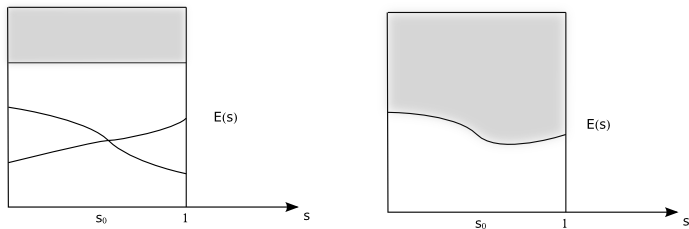
\includegraphics[width=.80\textwidth]{fig4.png}
\end{center}
\begin{enumerate}[1)]
\item
$P(s)$ sei spektraler Projektor zu $E(s)$ für $s\neq s_0$ und $E(s)$ sei diskreter Eigenwert (links).
\item Eingebetteter Eigenwert (rechts).
$E(s)=\inf \sigma(H(s))$ ein Eigenwert endlicher Vielfachheit und sei $P(s)$ Eigenprojektor zu $E(s)$.
\end{enumerate}

\chapter{Schrödingeroperatoren}\label{5}

\section{Multiplikations- und Differentialoperatoren}
Sei $( \Omega, \mu)$ ein $\sigma$-endlicher Maßraum (z.B. $\Omega = \R^n$, $\mu$ das Lebesgue-Maß). Sei $f: \Omega \to \C$ messbar und sei
\[
M_f : D(M_f) \subset L^2( \Omega) \to L^2( \Omega)
\]
definiert durch $M_f \phi:= f\phi$ wobei $D(M_f)=\{ \phi \in L^2| f\phi \in L^2(\Omega)\}.$

\begin{st}\label{5.1}
\begin{enumerate}[a)]
\item $M_f$ ist dicht definiert und $M_{\bar f} = M_f^*$
\item Das Spektrum von $M_f$ ist der wesentliche Wertebereich von $f$, d.h.
\[
\sigma(M_f) =\{z\in \C| \forall \eps >0, \mu(f^{-1} (B_\eps (z))>0\}
\]
\end{enumerate}
\begin{nt*}
Falls $f\in L^\infty(\Omega)$, dann 
\[
D(M_f) = L^2(\Omega) \text{ und } \| M_f\| \le \| f\|_\infty.
\]
\end{nt*}
\end{st}
\begin{proof}
siehe Satz 3.1 im Vorlesungsskript.
\end{proof}

\section{Differentialoperatoren}
Sei $\mathcal F: L^2(\R^n) \to L^2(\R^n)$ die Fouriertransformation und sei $f: \R^n \to \C$ messbar. Definiere den Operator
\[
-i \nabla = \mathcal F^{-1} M_f \mathcal F, \quad f(p)=p.
\]
\begin{align*}
D(-i \nabla)&=\{\phi \in L^2| \hat \phi \in D(M_f)\}\\
&=\{ \phi \in L^2| f \hat \phi \in L^2( \Omega)\}.
\end{align*}
Dann ist nach Satz \ref{5.1}, $-i \nabla$ dicht definiert, abgeschlossen und $\sigma(-i\nabla)=\sigma(M_f)$.

Der \emph{Laplace-Operator} $\Delta$ definiert durch
\[
- \Delta = \mathcal F^{-1} M_f \mathcal F, \quad f(p)=p^2
\]
\[
D(-\Delta)=\{\phi \in L^2| \int| p^2 \hat \phi (p)|^2 \, \dx[p] < \infty\}=H^2(\R^n).
\]
ist selbstadjungiert und $\sigma(- \Delta) = [0, \infty)$. Die \emph{Resolvente} $R(z)=(z+\Delta)^{-1}$ ist gegeben durch
\[
R(z)=\mathcal F^{-1} \frac{1}{z-p^2} \mathcal F.
\]    
Für $n\le 3$ ist $\hat G_z(p):= (z-p^2)^{-1}$ quadrat-integrierbar. Somit ist $G_z:=F^{-1} \hat G_z \in L^2(\R^n)$ und es gilt (Übung)
\[
(R(z) \phi)(x)=\int G_z(x-y) \phi(y) \, \dx[y].
\]
Für $n=3$ und $z\in \C\setminus [0,\infty)$ ist
\[
G_z(x) = \frac{1}{4\pi |x|} e^{-\sqrt{-z}|x|}, \quad \Re \sqrt{-z} >0.
\]
Die \emph{unitäre Gruppe} $U(t)$ welche durch $- \Delta$ erzeugt wird ist gegeben durch
\[
U(t)=\mathcal F^{-1} e^{ip^2 t} \mathcal F.
\]
Für $\psi \in L^1\cap L^2(\R^n)$ und $\pm t >0$ gilt
\[
(U(t)\psi)(x)=\frac{e^{\mp i \pi}}{(4\pi |t|)^{n/2}} \int e^{i(x-y)^2/(4t)} \psi(y) \, \dx[y].
\]

\section{Sobolevräume}
Für $s\ge 0$ definieren wir
\[
H^s(\R^n) = \{u \in L^2| |p|^s \hat u(p) \text{ ist quadratintegrierbar}\}
\]
und für $u,v\in H^s(\R^n)$
\[
\langle u, v \rangle_S = \int \overline{\hat u(p)} \hat v(p) (1+p^2)^s \, \dx[p].
\]
Nach Plancherel ist $H^0(\R^n)=L^2(\R^n)$ und
\[
s>t \ge 0 \implies H^s(\R^n) \subset H^t(\R^n) \subset L^2(\R^n).
\]
\begin{lem}\label{5.2}
Sei $\hat u: \R^n \to \C$ eine gegebene $L^1$-Funktion und sei $k\in \N$. Falls $|p|^k \hat U(p)$ integrierbar ist, dann ist
\[
u(x)=\int e^{ipx} \hat u(p) \, \dx[p]
\]
stetig und $k$ Mal stetig differenzierbar und
\[
\partial^\alpha u(x) = \int e^{ipx} (ip)^\alpha \hat u (p) \, \dx[p]
\]
für $|\alpha| \le k$ mit$\alpha=(\alpha_1,..., \alpha_n) \in \N_0^n$.
\end{lem}
\begin{proof}
Übung: Verwende Riemann-Lebesgue, Lebesgue Majorisierte Konvergenz und $|e^{is} -1|\le |s|$.
\end{proof}

\begin{st}[Sobolev-Lemma]\label{5.3}
Sei $u\in H^s(\R^n)$ und $k\in \N_0$ mit $k<s- \frac{n}{2}$. Dann gilt für alle $\alpha: |\alpha|\le k$:
\begin{enumerate}[a)]
\item $u\in C^k(\R^n)$ und $\partial^\alpha u(x) \to 0$ für $|x|\to \infty$;
\item $\sup_x |\partial^\alpha u(x)| \le C_{k,s,n} \|u\|_s.$
\end{enumerate}
\end{st}
\begin{proof}
Übung: Zeige, dass $|p|^k \hat u(p)$ integrierbar ist und verwende Lemma \ref{5.2}. Siehe auch Satz 3.3 aus dem Vorlesungsskript.
\end{proof}

\begin{ex*}
Wir wissen, dass $H^2(\R^2)=D(-\Delta)$ und nach Satz \ref{4.3} gilt:
\begin{itemize}
\item $\phi \in H^2(\R^3) \implies \phi \in C(\R^3)$ und $\phi(x)\to 0$ ($|x|\to \infty$),
\item $\phi \in H^1(\mathbb R)\implies \phi \in C^1(\mathbb R)$ und $\phi(x), \phi'(x)\to 0$ ($|x|\to \infty$).
\end{itemize}
\end{ex*}


\begin{st} 
$H^s(\R^n)$ ist ein Hilbertraum und $C_0^\infty$ ist dicht in $H^s(\R^n)$.
\end{st}
\begin{proof}
Übung, oder Literatur (z.B. Rudin).
\end{proof}
\begin{df}
Sind $u,v\in L^1_{\text{loc}}(\R^n)$ und $\alpha \in \N_0^n$, dann heißt $v$ \emph{schwache $\alpha$-Ableitung} von $u$, wir schreiben $v=\partial^\alpha u$, wenn für alle $\phi \in C_0^\infty (\R^n)$ gilt
\[
(-1)^{|\alpha|} \int \partial^\alpha \phi(x) u(x) \, \dx = \int \phi(x) v(x) \, \dx.
\] 
Die schwache $\alpha$-Ableitung ist eindeutig, denn aus $\int \phi v \, \dx=0$ für alle $\phi \in C_0^\infty$ folgt $v(x)=0$ fast überall. (Fundamentallemma der Distributionstheorie).
\end{df}

\begin{st}\label{5.5}
Sei $\alpha\in \N_0^n$ und $u\in L^2(\R^n)$. Dann sind äquivalent:
\begin{enumerate}[a)]
\item$u$ hat eine schwache $\alpha$-Ableitung $\partial^\alpha u\in L^2$.
\item $p \mapsto p^\alpha \hat u(p)$ ist quadratintegrierbar.
\end{enumerate}
Gilt a) oder b) dann $\partial^\alpha u = \mathcal F^{-1} (ip)^\alpha \mathcal Fu$.
\end{st}
\begin{proof}
Sei $D^\alpha$ der s.a. Operator definiert durch
\[
\mathrm D^\alpha = \mathcal F^{-1} p^\alpha \mathcal F.
\]
Hierbei sei 
\[
D(\mathrm D^\alpha) = \{ u \in L^2| p^{\alpha} \hat u(p) \text{ ist in } L^2\}
\]
der Definitionsbereich von $\mathrm D^\alpha$. Aus b) folgt $u\in D(\mathrm D^\alpha)$ und für alle $\phi \in C_c^\infty(\R^n)$ gilt
\[
\< \phi, \mathrm D^\alpha u\>= \< D^\alpha \phi, u\>,
\]
was äquivalent ist zu (a). Umgekehrt folgt aus (a), dass für alle $\phi \in C_0^\infty(\R^n)$ gilt:
\[
(-1)^{|\alpha|} \int \overline{\partial^\alpha \phi(x)} u(x) \, \dx = \int \overline{\phi(x)} \partial^\alpha u(x) \, \dx
\]
was äquivalent ist zu
\[
\langle \mathrm D^\alpha \phi, U \rangle = \langle \phi, \partial^\alpha u \rangle (-i)^{|\alpha|}
\]
für alle $\phi \in C_0^\infty(\R^n)$. Daraus folgt
$\big(\mathrm D^\alpha\upharpoonright C_0^\infty(\R^n)\big)^*u= (-i)^{|\alpha|} \partial^\alpha u$. Es genügt zu zeigen, dass
\[
D^\alpha = \overline{\mathrm D^\alpha \upharpoonright C_0^\infty(\R^n)},
\]
d.h. dass $\mathrm D^\alpha \upharpoonright C_0^\infty(\R^n)$ wesentlich s.a. ist. (Übung)
\end{proof}

\begin{st}\label{5.6}
Sei $u\in L^2(\R^n)$, $m\in \N$ und für alle $\alpha\in \N_0^n, |\alpha|\le m$ existiere die schwache $\alpha$-Ableitung $\partial^\alpha u$ und $\partial^\alpha u\in L^2$. Dann ist $u\in H^m(\R^n)$.  
\end{st}
\begin{proof}
Nach Satz \ref{5.5} ist $p^\alpha \hat u(p)$ quadratintegrierbar für alle $|\alpha|\le m$ und mit $|p|^m \hat u(p)$ quadratintegrierbar, also $u\in H^m$.
\end{proof}

\begin{kor}\label{5.7}
$C_0^m(\R^n) \subset H^m(\R^n)$
\end{kor}

\begin{st}\label{5.8}
Sei $u\in H^m(\R^n)$, $f\in C^m(\R^n)$ wobei alle Ableitungen $\partial^\alpha f, |\alpha| \le m$, in $L^\infty(\R^n)$ sind. Dann gilt $fu \in H^m$,
$\|fu\|_m\le C_f \| u\|_m$ und es gilt die Leibnizformel
\[
\partial^\alpha(fu)=\sum_{\beta \le \alpha} \binom{\alpha}{\beta} \partial^\beta f \partial^{\alpha- \beta} u.
\]
\end{st}
\begin{proof}
Wir setzen $\| u \|_{m,2}=\sum_{|\alpha| \le m} \| \partial^\alpha u\|_{L^2}$.

Diese Norm ist äquivalent zur Norm von $H^m$. Für $\phi \in C_0^\infty(\R^n)$ gilt
\begin{equation}\label{4.1}
\delta^\alpha(f\phi) = \sum_{\beta \le \alpha} \binom{\alpha}{\beta} \delta^\beta f \delta^{\alpha-\beta} \phi
\end{equation}
und somit
\begin{align*}
\|\delta^\alpha(f\phi) \|_2 &\le \sum_{\beta \le \alpha} \binom{\alpha}{\beta} \| \delta^\beta f\| _{L^2} \| \delta^{\alpha-\beta} \phi \|_{L^2}\\
&\le C_{\alpha,f} \sum_{|\alpha|\le m} \| \delta^\alpha \phi \|_{L^2}= C_{\alpha,f} \| \phi \|_{m,2}.
\end{align*}
Daraus folgt
\[
\|f\phi\|_{m,2}= \sum_{|\alpha|\le m} \| \delta^\alpha(f\phi)\|_2=\underbrace{\left (\sum_{|\alpha|\le m} C_\alpha,f\right) }_{C_f}  \|\phi\|_{m,2}
\]
Somit ist $M_f:C_0^\infty (\R^n) \subset H^m \to H^m$ eine beschränkte lineare Abbildung. Sie hat eindeutige beschränkte Fortsetzung auf $H^m$, welche ebenfalls durch  Multiplikation mit $f$ gegeben ist. (Details dazu in Skript) Die Leibniz-Formel auf $H^m$ folgt nun aus \eqref{4.1} durch ein Approximationsargument.
\end{proof}

\section{Schrödingeroperatoren}

Wir betrachten Operatoren der Form $-\Delta+V:D\subset L^2(\R^n) \to L^2(\R^n)$, wobei $V=M_V$ Multiplikationsoperator ist. Wir schreiben $V\in L^2(\R^n)+L^\infty(\R^n)$, falls sich $V$ darstellen lässt als $V=V_2+V_\infty$ mit $V_2\in L^2$ und $V_\infty \in L^\infty$.

\begin{ex*}[Coloumbpotential]
Betrachte
\[
V(x)=\begin{cases} - \frac{1}{|x|}&, x\in \R^3\setminus\{0\}\\ 0&, x=0 \end{cases}
\]
Offenbar liegt $V(x)$ in der Klasse $L^2+L^\infty$, denn für $\eps>0$ sei $\chi$ die charakteristische Funktion auf $\{|x|<\eps\}$, setze $V_2:= V \cdot \chi$ und $V_\infty:= V\cdot (1-\chi)$. Dann gilt $\|V_\infty\|_\infty=\eps^{-1}$ und $\|V_2\|=\sqrt{4\pi \eps}$.
\end{ex*}

\begin{lem}
Ist $V\in L^2(\R^n)$, dann existiert für jedes $\eps>0$ eine Zerlegung $V_2+V_\infty$ mit $\| V_2\| <\eps$.
\end{lem}
\begin{proof} %\fixme
Sei $\chi_N$ die charakterische Funktion auf $\{x\in \R^n| |V(x)|\le N\}$ für $N \in \N$. Daraus folgt
\[
|V|^2 \ge |V|^2(1-\chi_N) \to 0
\]
für $N\to \infty$ und $|V|^2 \in L^1(\R^n)$. Also
\[
\int |V(x)|^2 (1- \chi_N) \, \dx \to 0
\]
für $N\to \infty$ mit dem Satz von Lebesgue. Wähle $N$ nun groß genug, sodass $\int | V(x)|^2 (1- \chi_n) \le \eps^2$ und setze $V_2:= V(1-\chi_N) $ mit $\| V_2\| < \eps$ und $V_\infty := V\chi_N \in L^\infty$.
\end{proof}
\begin{st}\label{5.11}
Sei $V\in L^2+ L^\infty$ und $n\ge 3$. Zu jedem $\eps >0$ existiert ein $C_\eps>0$ mit
\begin{equation}\label{4.2}
\| V\phi\| \le \eps \| \Delta \phi\| + C_\eps \| \phi\| 
\end{equation}
für alle $\phi \in C_0^\infty$. Wenn $V$ reellwertig ist, dann ist $-\Delta+V$ selbstadjungiert auf $H^2(\R^n)$ und wesentlich selbstadjungiert auf $C_0^\infty(\R^n)$.
\end{st}
\begin{proof}
Siehe Vorlesungskript Theorem 3.5.
\end{proof}

\subsection{Schrödingeroperatoren von Atome und Molekülen}
Wir betrachten statische Kerne von Atomen. Sei der Schrödingeroperator gegeben durch
\begin{equation}\label{4.3}
- \Delta+ \sum_{k=1}^N V_k + \sum_{i<k} V_{ik},
\end{equation}
wobei $N$ die Anzahl der Elektronen sei. Hierbei beschreibt $V_k$ die Wechselwirkung der Elektronen mit den statischen Kernen und $V_{ik}$ die Wechselwirkung zwischen den Elektronen. $V_k$ und $V_{ik}$ sind Multiplikationsoperatoren der Form
\begin{align*}
(V_k \cdot \phi)(x_1,...,x_N)&:= V(x_k) \phi(x_1,...,x_N), x_1, ...,x_N \in \R^3\\
(V_{ik} \cdot \phi)(x_1,...,x_N)&:= W(x_i-x_k) \phi(x_1,..., x_N)
\end{align*}
\begin{thm}[Kato 1951]\label{5.12}
Falls $V,W\in L^2+L^\infty(\R^3)$ dann ist \eqref{4.3} selbstadjungiert auf $H^2(\R^{3N})$ und wesentlich selbstadjungiert auf $C_0^\infty(\R^{3N})$.
\end{thm}
\begin{proof}
Sei $\phi\in C_0^\infty(\R^{3N})$. Sei o.B.d.A. $k=1, i=2$. Dann ist
\begin{align*}
\|V_1 \phi \|_{L^2(\R^{3N}} &\le \eps \| \Delta_1 \phi \|_{L^2(\R^{3N})} + C_\eps \| \phi \| {L^2(\R^{3N})} \\
 &\le \eps \| \Delta \phi \|_{L^2(\R^{3N})}+ C_\eps \| \phi \|_{L^2(\R^{3N})}
\end{align*}
denn $\| \Delta_1 \phi \| \le \| \Delta \phi \|$ (folgt aus Fourierdarstellung des $-\Delta$) und
\begin{align*}
\| V_1 \phi \|^2 &= \int \dx[x_N] ... \int \dx[x_1] |V(x_1)|^2 | \phi(x_1,\cdot)\|^2\\
&= \| V_1(\phi(x_1,\cdot)\|^2_{L^2(\R^{3N})} \stackrel{\text{Satz } \ref{5.11}}\le 2\eps^2 \|\Delta_1 \phi\|^2 + 2c_\eps^2 \| \phi \|^2_{L^2(\R^3)}.
\end{align*}
Analog folgt 
\[
\|V_k \phi \|_{L^2(\R^{3N})} \le \eps \| \Delta \phi \|_{L^2(\R^{3N})} + C_\eps \| \phi \|_{L^2(\R^{3N})}
\]
für alle $k$. Auf die gleiche Weise zeigt man 
\[
\|V_{21} \phi \| \le \eps \| \Delta \phi \|_{L^2(\R^{3N})} + C_\eps \| \phi \|_{L^2( \R^{3N})}
\]
und es folgt
\[
\| V_{ik} \phi\| \le \eps \| \Delta \phi \| + C_\eps \| \phi \|. 
\]
Also %\fixme
\begin{align*}
\Bigg \|\bigg ( \sum_{k=1}^N V_k &+ \sum_{i<j} V_{ik}\bigg) \phi \Bigg \|^2_{L^2(\R^{3N})}
\\ &\le \big (\frac{N(N+1)}{2}\big)^2 \eps \| \Delta \phi \|^2_{L^2(\R^{3N})} + \big ( \frac{ N(N+1)}{2} \big )^2 C_\eps \| \phi \|^2_{L^2(\R^{3N})}.
\end{align*}
%Wobei wir an der einen oder anderen Stelle ausnutzen, dass $\sqrt{a+b} \le \sqrt{a} + \sqrt{b}$ für $a,b\in \R$ gilt.
\end{proof}

\begin{kor}
Der Schrödingeroperator eines Atoms mit $N$ Elektronen und Atomzahl $z$,
\[
H_{N,z} = \sum_{k=1}^N \big ( - \frac{\hslash^2}{2m} \Delta_{x_k} - \frac{z_e^2}{|x_k|}\big) + \sum_{i<k} \frac{e^2}{|x_i-x_k|}
\]
ist selbstadjungiert auf $H^2(\R^{3N})$ und wesentlich selbstadjungiert auf $C_0^\infty(\R^{3N})$. Dabei sei $\hslash$ das Planksche Wirkungsquantum $\hslash=\frac{h}{2\pi}$ und $m$ die Masse des Elektrons und $e$ die Elementarladung.
\end{kor}
\subsection{Bemerkung zu den Einheiten}
Der Operator $H_{N,z}$ aus Korrolar \ref{5.7} unitär äquivalent ist zu 
\[
2\alpha^2 mc^2 \bigg[ \sum_{k=1}^N \big ( - \Delta_{x_k} - \frac{z}{|x_k|} \big ) + \sum_{i<k} \frac{1}{|x_i-x_j|} \bigg ]
\]
wobei $\alpha=\frac{e^2}{\hslash c} \approx \frac{1}{137}$ die \emph{Feinstrukturkonstante}. Wir definieren
\[
U:L^2(\R^{3N} \to L^2(\R^{3N}), \quad (U\phi) (x) := \lambda^{\frac{3}{2}N} \phi(\lambda x); \lambda>0.
\]
$U$ ist isometrisch und bijektiv, also \emph{unitär}. Es folgt
%\fixme
\[
U H_{N,z} U^{-1} = \sum_{k=1}^N \big(- \frac{\hslash^2}{2m\lambda^2} \Delta_{x_k} - \frac{z e^2}{\lambda|x_k|} \big ) + \sum_{i<k} \frac{e^2}{\lambda|x_i-x_k|}.
\]
Wähle $\lambda$, sodass
\[
\frac{\hslash^2}{2m \lambda^2} \stack!= \frac{e^2}{\lambda} 
\]
und damit $\lambda= \frac{\hslash^2}{2me^2}$.

\chapter{Funktionalkalkül und Spektralsatz}\label{6}

\section{Messbarer Funktionalkalkül}
Bezeichne $B$ die Borelmessbaren Teilmenge von $\R$. und $\mathcal B(\R)$ die Familie der beschränkten Borelmessbaren Funktionen $f: \R \to \C$. Definiere dazu
\[
\| f\|_\infty = \sup_{x\in \R} |f(x)|
\]
Ist $(f_n)$ eine Folge in $\mathcal B(\R)$ mit $\sup_{n} |f_n(x)| < \infty$ und $f_n(x) \to f(x)$ für $n\to \infty$ für alle $x\in \mathbb R$. Dann schreiben wir $f_n \stack{\text{p}}\to f$.
\begin{st}\label{6.1}
Sei $A:D(A) \subset H \to H$ selbstadjungiert. Dann gibt es eine eindeutig beschränkte Abbildung $\Phi: \mathcal B(\R) \to \mathcal L(H)$ mit
\begin{enumerate}[(1)]
\item Ist $z\in \C\setminus\R$ und $f_z(x) = (z-x)^{-1}$ dann
\[
\Phi(f_z) =(z-A)^{-1}
\]
\item Für alle $f,g \in \mathcal B(\R)$, $\alpha, \beta\in \C$ gilt:
\begin{align*}
\Phi(\alpha f + \beta g)&= \alpha \Phi(f)\\
\Phi(fg) &= \Phi(f) \Phi(g)\\
\Phi(f)^* &= \Phi(\bar f)
\end{align*}
\item Falls $f_n \stack{\text{p}}\to f$, dann gilt $\Phi(f_n) \phi \to \Phi(f) \phi$ für alle $\phi \in H$.
\end{enumerate}
Weiterhin gilt für alle $f\in \mathcal B(R)$:
\begin{enumerate}
\item[(4)] $\| \Phi(f)\| \le \|f\|_\infty$
\item[(5)] Aus $f\ge 0$ folgt $\Phi(f) \ge 0$. 
\end{enumerate}
\end{st}
\begin{proof}
vgl. Vorlesung Spektraltheorie. %(\fixme[bessere Quelle?])
\end{proof}

\begin{ex*}
Sei $A: D(A) \subset L^2(\R)\to L^2(\R)$ definiert durch
\[
D(A) = \{\phi \in L^2|\, \int |x\phi(x)|^2 \, \dx <\infty\}, \quad (A\phi) (x) = x \phi(x).
\]
Dann ist $\Phi(f)=M_f$ der Multiplikationsoperator.
\end{ex*}
\begin{proof}
Es genügt zu zeigen, dass $f\mapsto M_f$ die Eigenschaften (1)-(3) aus Satz \ref{6.1} hat.
\end{proof}

Die Abbildung $P: B \to \mathcal L(H)$ mit
\[
P_\Omega= \Phi(\chi_\Omega), \quad \Omega \in B
\]
heißt \emph{Spektralmaß} von $A$. Das Spektralmaß ist ein projektionswertiges Maß.

\section{Projektionswertige Maße}
Ein projektionswertiges Maß (p.w.M.) ist eine Abbildung $P: B \to \mathcal L(H)$ mit
\begin{enumerate}[(1)]
\item $P_\Omega$ ist Orthogonalprojektor, d.h. $P_\Omega^2 = P_\Omega$ und $P_\Omega^* = P_\Omega$
\item $P_\emptyset=0$ und $P_\Omega =\mathbb 1$
\item Falls $\Omega = \bigcup_{k=1}^\infty \Omega_k$ und $\Omega_i \cap \Omega_j=\emptyset$ für $i\neq j$, dann ist
\[
P_\Omega \phi = \lim_{N\to \infty} \sum_{k=1}^N P_{\Omega_k} \phi.
\] 

\end{enumerate} 
$\mu_\phi(\Omega)=\< \phi, P_\Omega \phi \>$ ist ein Borelmaß auf $\R$. (wenn $\|\phi \|=1$, dann sogar ein Wahrscheinlichkeits-Maß) und aus (1)-(3) folgt $P_\Omega P_{\Omega'}= P_{\Omega \cap \Omega'}$ (Übung).

Ausserdem ist jedes p.w.M. monoton und subadditiv, d.h.
\begin{align*}
\Omega_1 \subset \Omega_2 &\implies P_{\Omega_1} \le P_{\Omega_2}\\
\Omega= \bigcup_{k=1}^N \Omega_k &\implies P_\Omega \le \sum_{k=1}^N P_{\Omega_k},
\end{align*}
wobei 
\[
P_{\Omega_1} \le P_{\Omega_2} \iff \mu_\phi(\Omega_1) \le \mu_\phi (\Omega_2) \quad \forall \phi \in H.
\]
Ist $s= \sum_{k=1}^N \alpha_k \chi_{E_k}$ eine messbare Elementarfunktion in Standarddarstellung (d.h. $E_k = s^{-1}(\{\alpha_k\})$, dann bezeichne
\[
\int s dP:= \sum_{k=1}^N \alpha_k P_{E_k}.
\]

Die Abbildung $s\mapsto \int s dP$ ist linear und es gilt $\| \int s dP \| \le \| s\|_\infty$. (Beweis s. z.B. Werner Funktionalanalysis)

Da messbare Elementarfunktionen dicht sind in $B(\R)$ bezüglich $\| \cdot \|_\infty$ lässt sich die Integration bezüglich $P$ ausdehen auf alle Funktionen $f\in \mathcal B(\R)$. D.h.
\[
\int f \, \dx[P] = \lim_{n\to \infty} \int s_n \, \dx[P]
\]
wobei $(s_n)$ eine beliebige Folge messbarer Elementarfunktionen ist mit $\| s_n-f\|_\infty\to 0$ für $n\to \infty$. Man schreibt auch $\int f(\lambda) \, \dx[P]$ für $\int f \,\dx[P]$ und
\[
\int_\Omega f \, \dx[P] := \int f \chi_\Omega \, \dx[P].
\]
Man zeigt nun leicht, dass
\begin{enumerate}[a)]
\item $\int f \chi_\Omega \, \dx[P] = (\int f \, \dx[P]) P_\Omega = P_\Omega ( \int f \, \dx[P])$,
\item $\int fg \, \dx[P]= (\int f \, \dx[P]) (\int g \, \dx[P])$, 
\item $(\int f \, \dx[P])^*= \int \overline{f} \, \dx[P]$.
\end{enumerate}
(Beweis sieh z.B. Werner Funktionalanalysis)

Der \emph{Träger} $\supp(P)$ eines p.w.M. ist definiert durch $\lambda \in \supp(P)$ genau dann wenn
$P_U\neq 0$ für jede Umgebung $U\ni \lambda$.
\begin{st}
Sei $P$ ein p.w.M. Dann gilt:
\begin{enumerate}
\item $S:= \supp(P)$ ist abgeschlossen
\item $P_S= \mathbb{1}$ und  $P_{\R \setminus S} =0$.
\item Für jede Funktion Funktion $f\in \mathcal B(\R) \cap C(\R)$ gilt
\[
\left \| \int f\, \dx[P]\right \| = \sup_{x\in \R} |f(x)|
\]
\end{enumerate}
\end{st}
\begin{proof}
siehe Lemma 7.5 aus dem Vorlesungsskript.
\end{proof}
\begin{st}
Sei $A=A^*$ mit Spektralmaß $P$, d.h. $P_\Omega= \Phi(\chi_\Omega)$, wobei $\Phi $ der Funktionalkalkül von $A$ ist. Dann gilt
\begin{enumerate}[a)]
\item $P$ ist ein p.w.M.,
\item $\supp(P) = \sigma(A)$,
\item $\| (z-A)^{-1} \| = \dist(z, \sigma(A))^{-1}$ für alle $z\in D(A)$,
\item für alle $f\in \mathcal B(\R)$ gilt
\[
\Phi(f) = \int f \, \dx[P].
\]

\end{enumerate}
\end{st}
\begin{proof}
siehe Satz 7.6 aus dem Vorlesungsskript.
\end{proof}

\section{Spektralsatz}
Für beliebige messbare $f: \R \to \C$ definieren wir einen (unbeschränkten) Operator $\Phi(f)$ durch
\begin{equation}\label{eq:6.1}
D(\Phi(f))= \Phi(\frac{1}{1+|f|}) H, \quad \Phi(f) \phi = \Phi(\frac{f}{1+|f|}) \gamma
\end{equation}
falls $\phi = \Phi(\frac{1}{1+|f|}) \gamma$.

\begin{st}
Sei $A^*=A$ mit Funktionalkalkül $\Phi$. Sei $\Phi$ für beliebige messbaren $f: \R \to \C$ definiert durch \ref{6.1}. Dann gilt
\begin{enumerate}[a)]
\item $\Phi(f)$ ist wohl- und dicht definiert.
\item Falls $f_k \in \mathcal B(\R)$, $|f_k|\le |f|$ und $f_k(x) \to f(x)$ für alle $x\in \R$. Dann gilt
\[
\Phi(f) \phi = \lim_{n\to \infty} \Phi(f_k) \phi
\]
für alle $\phi \in D(\Phi(f))$.
\item $D(\phi(f))=\{\phi \in H| \int |f|^2 \, \dx[\mu_\phi] < \infty\}$ und für $\phi, \psi \in D(\Phi(f))$ gilt
\[
\| \Phi(f) \phi\|^2 = \int |f|^2 \, \dx[\mu_\phi].
\]
und die Polarisationsidentität
\begin{align*}
\< \phi, \Phi(f) \psi\> &= \int f(\lambda) \, \dx[\mu_{\phi, \psi}] \\
&= \frac{1}{4} \left (\int f(\lambda) \, \dx[\mu_{\phi+\psi}] - \int f \, \, \dx[\mu_{\phi-\psi}]\right )\\
&\ \quad + \frac{1}{4i} \left (\int f \, \dx[\mu_{\phi+i\psi}] - \int f \, \dx[\mu_{\phi-i\psi}]\right ),
\end{align*}
wobei $\mu_\phi(\Omega):= \< \phi, P_\Omega \phi\>$. 
\item Falls $g, fg \in B(\R)$, dann ist $\Phi(g) H \subset D(\phi(f))$ und
\[
\Phi(f) \Phi(g) = \Phi(fg).
\]
\item $\Phi(f)^*= \Phi(\overline f)$ und $\Phi(\Id) =A$ wenn $\Id(x) = x$
\end{enumerate}
\end{st}
\begin{proof}
Siehe Vorlesungsskript Satz 7.9.
\end{proof}

\begin{nt*}
\begin{enumerate}[1)]
\item Der Spektralsatz $\Phi(\Id)=A$ (zusammen mit d), d.h. $\< \phi, A\psi\> = \int \lambda \, d\mu_{\phi, \psi}(\lambda)$ ist die Verallgemeinerung der Spektralzerlegung
\[
	A= \sum_{k=1}^m \lambda_k P_k
\]
eines selbstadjungierten Operatores $A\in \mathcal L(\C^n)$ mit Eigenwerten $\lambda_1,...,\lambda_m \in \R$ mit Eigenprojektoren $P_k$.
\item $A$ ist genau dann beschränkt wenn $\sigma(A)$ beschränkt ist und $\| A \| = \sup_{\lambda \in \sigma(A)} | \lambda | = \sup_{\| \phi \| = 1} | \< \phi, A\phi\>|$.
\item $P_\Omega A\subset A P_\Omega$, $A\upharpoonright H_\Omega := P_\Omega H$ ist selbstadjungiert mit Definitionsbereich $P_\Omega D(A)$ und wenn $\Omega \subset \R$ offen ist, dann ist 
\[
	\sigma(A) \cap \Omega \subset \sigma(A \upharpoonright H_\Omega) \subset \sigma(A) \cap \overline{\Omega}.
\]
\item $\lambda \in \R$ ist genau dann Eigenwert von $A$ wenn $P_{\{\lambda\}} \neq 0$. Dann ist $P_{\{\lambda\}}$ der Orthogonalprojektor auf den Eigenraum zu $\lambda$.
\item Statt $\Phi(f)$ schreibt man oft $f(A)$. Dalls $A\phi= \lambda \phi$ dann ist
\[
f(A) \phi = f(\lambda) \phi.
\]
\item In der Quantenmechanik wird jede beschränktbare Größe durch ein selbstadjungierten Operator $A$ in einem Hilbertraum $H$ beschrieben. Die normierten Vektoren $\phi \in H$ beschreiben (reine) Zustände des Systems. Ist $\Omega \subset \R$ eine Borelmenge, dann ist
\[
\mu_\phi(\Omega) = \< \phi, P_\Omega \phi \>.
\]
Die Wahrscheinlichkeit bei einer Messung der Observablen $A$ in einem Zustand $\phi''$ einen Wert in $\Omega$ zu finden. Wegen $\mu_\phi(\R\setminus \sigma(A))=0$ können nur Messwerte in $\sigma(A)$ gefunden werden. Der Erwartungswert
\[
\int \lambda \, \dx[\mu_\phi(\lambda)] = \< \phi, A\phi\>
\]
kann allerding einen beliebigen Wert zwischen $\inf\sigma(A)$ und $\sup \sigma(A)$ annehmen.
\end{enumerate}
\end{nt*}







\begin{st}\label{6.5}
Sei $A^*=A$ und $\sigma \subset \sigma(A)$, kompakt mit $\dist(\sigma, \sigma(A)\setminus \sigma)>0$. Sei $\gamma$ eine $C^1$-Kurve welche $\sigma$ ein Mal umläuft und $\sigma(A)$ nicht schneidet. Dann gilt
\[
P_\sigma=\frac{1}{2\pi i} \int_\gamma (z-A)^{-1} \, \dx[z],
\]
wobei $P$ das Spektralmaß zu $A$ ist.
\end{st}
\begin{proof}
Für ale $x\in \sigma(A)$ gilt
\[
\chi_\sigma(\lambda) = \frac{1}{2\pi i} \int_\gamma (z-\lambda)^{-1} \, \dx[z]
\]
also für alle $\lambda\in \R$. Insbesondere gilt 
\[
\chi_\sigma(\lambda) = \frac{1}{2\pi i} \int_\gamma (z-\lambda)^{-1} \chi_{\sigma(A)} (\lambda) \, \dx[z].
\]
Also
\begin{align*}
P_\sigma &= \Phi(\chi_\sigma)=\Phi(\frac{1}{2\pi i}) \int_\gamma (z-\lambda)^{-1} \chi_{\sigma(A)}(\lambda) \, \dx[z]\\
&= \frac{1}{2\pi i} \int_\gamma \Phi((z-\lambda)^{-1} \chi_{\sigma(A)} (\lambda)) \, \dx[z] \\
&= \frac{1}{2\pi i} \int_\gamma \Phi(\frac{1}{z-\lambda}) \Phi(\chi_{\sigma(A)}) \, \dx[z] \\
&= \frac{1}{2\pi i} \int_\gamma (z-A)^{-1} \, \dx[z],
\end{align*}
wobei wir ausnutzen, dass $f_n \stack{p}\to f$ und $\phi(f_n) \phi \to \phi(f) \phi$. Es gilt also
\begin{align*}
\int_\gamma (z-\lambda)^{-1} \chi_{\sigma(A)} (\lambda) \, \dx[z] = \lim_{N\to \infty} \sum_{i=1}^N (\gamma(t_i) - \lambda)^{-1} \chi_{\sigma(A)}(\lambda) \dot \gamma(t_i) \Delta t
\end{align*}
wobei
\[
\Big | \sum_{i=1}^N (\gamma(t_i) - \lambda)^{-1} \chi_{\sigma(A)}(\lambda) \dot \gamma(t_i) \Delta t \Big | \le \frac{1}{\dist(\Tr(\gamma), \sigma(A))} (L(\gamma)+1)
\]
für $N$ hinreichend groß und $L$ die Länge von $\gamma$. Also gilt
\begin{align*}
\Phi(\int_\gamma (z-\lambda)^{-1} \chi_{\sigma(A)} \, \dx[z]) \phi&= \lim_{N\to \infty} \sum_{i=1}^N \Phi((\gamma(t_i)-\lambda)^{-1} \chi_\sigma(A)) \dot \gamma(t_i) \Delta t \phi \\
&= \lim_{N\to \infty} \sum_{i=1}^N (\gamma(t_i) -A)^{-1} \dot \gamma(t_i) \Delta t \phi\\
&= \int (z-A)^{-1} \, \dx[z] \phi
\end{align*} 
Was letztendlich den Beweis abschließt.
\end{proof}

\begin{seg}[Erinnerung]
$\lambda \in \sigma_{\text{disc}}(A)$ falls $\lambda \in \sigma(A)$, $B_\eps(\lambda) \cap \sigma(A)=\{\lambda\}$, und falls 
\[
\dim(\frac{1}{2\pi i} \oint_{|z-\lambda|= \eps/2} (z-A)^{-1 } \, \dx[z]) H < \infty
\]
genau dann wenn $\dim(P_{\{\lambda\}}H)<\infty$ nach Satz \ref{6.5}. %\fixme
\end{seg}
\begin{thm}
Sei $A^*=A$ und $P$ das Spektralmaß von $A$. Dann gilt:
\begin{enumerate}[a)]
\item $\lambda \in \sigma(A)$ genau dann wenn $P_{(\lambda- \eps, x+ \eps)}\neq 0$ für alle $\eps>0$.
\item $\lambda \in \sigma_{\text{disc}}(A)$ genau dann wenn es ein $\eps>0$ gibt, so dass $\dim P_{(\lambda-\eps, \lambda+\eps)} H<\infty$.
\item $\lambda \in \sigma_{\text{ess}}(A)$ genau dann, wenn $\dim P_{(\lambda-\eps, \lambda + \eps)} H = \infty$ für alle $\eps>0$. 
\end{enumerate}
\end{thm}
\begin{proof}
\begin{enumerate}[a)]
Nach Theorem 3 gilt $\sigma(A)=\supp(P)$. Also ist $\lambda \in \sigma(A)$ genau dann wenn $\lambda \in \supp(P)$, genau dann wenn $P_u\neq 0$ für jede Umgebung $\lambda \in U$, genau dann wenn $P_{(\lambda-\eps, \lambda + \eps)} \neq 0$ für alle $\eps>0$.
\item Es ist $x\in \sigma_{\text{disc}}(A)$ genau dann gilt, wenn $\lambda \in \sigma(A)$ und es ein $\eps>0$ gibt mit $B_\eps(\lambda)\cap \sigma(A)=\{\lambda\}$ und $\dim P_{\{\lambda\}} H < \infty$.
Also wenn $\lambda \in \sigma_{\text{disc}}(A)$, dann existiert ein $\eps>0$ mit $P_{(\lambda-\eps, \lambda + \eps)}= P_{\{\lambda\}}$. Also ist $\dim P_{(\lambda- \eps, \lambda + \eps)} H < \infty$. Dann gilt
\[
\sigma(A) \cap B_{\eps}(\lambda) \subset \sigma(A \upharpoonright P_{(\lambda-\eps, \lambda+\eps)}H) = \{\lambda_1,..., \lambda_m\}
\]
wobei $\sigma(A) \cap B_{\eps}(\lambda) \subset \sigma(A \upharpoonright P_{(\lambda-\eps, \lambda+\eps)}H)$ eine Folgerung zu dem Spektralsatz ist für $m\le n$ (Beweis Übung).
Also ist $\lambda \in \sigma_{\text{disc}}(A)$
\item $\lambda \int \sigma_{\text{ess}}(A)$ genau dann wenn $\lambda \in \sigma(A) \setminus \sigma_{\text{disc}} (A)$, was nach a) und b) gerade gleichbedeutend zu $\dim(P_{(\lambda-\eps, \lambda+\eps)} H)<\infty$
\end{enumerate}
\end{proof}


\begin{st}[Weyl]\label{6.7}
Sei $A^*=A$. Dann ist $\lambda \in \sigma_{\text{ess}}(A)$ genau dann, wenn eine Folge $(\phi_n)$ existiert mit $\phi_n\in D(A), \|\phi_n\|=1$ mit $\phi_n \rightharpoonup 0$ und $\|(A-\lambda) \phi_n\| \to 0$. Man nennt diese Folge auch \emph{Weyl-Folge}.
\end{st}

\begin{proof} %\fixme
Sei $\lambda\in \sigma_{\text{ess}}(A)$ und sei $P_n:= P_{(\lambda-1/n, \lambda+ 1/n)}$. Wir konstruieren \emph{rekursiv} eine Orthonormalfolge $(\phi_n)$ mit $\phi_n\in P_n H$: $\phi_1 \in P_1H$ sei normiert aber ansonsten beliebig. Sind $\phi_1, ..., \phi_{n-1}$ konstruiert, dann existiert $\phi_n \in P_n H \cap \{\phi_1... \phi_{n-1}\}^\perp$ mit $\|\phi_n \| =1$, denn $\dim P_n H=\infty$ nach Theorem 6. Es gilt $\phi_n \rightharpoonup 0$ mit $\phi_n \in D(A)$ und es folgt
\begin{align*}
\|(A-\lambda) \phi_n \| &\le \| (A-\lambda) P_n\| = \| \Phi(x-\lambda) \Phi(\chi_{(\lambda-1/n, \lambda+1/n)}) \|\\
&= \| \Phi((x-\lambda) \chi_{(\lambda-1/n), \lambda + 1/n)} \| \le \frac{1}{n} \to 0
\end{align*}
für $n\to \infty$. Sei nun $(\phi_n)$ eine Weylfolge und sei $\lambda \in \sigma_{\text{disc}} (A)$. Wir leiten einen Widerspruch her. Dann existiert zu einem $\eps >0$ mit $\dim P_\eps H<\infty$ wobei $P_\eps= P_{(\lambda-\eps, \lambda+\eps)}$ nach Theorem 6. Also gilt $P_\eps \phi_n \to 0$ für $n\to \infty$. (Übung)
Andererseits gilt
\[
\| (A-\lambda) \phi_n\|^2 \ge \| \underbrace{(1-P_\eps) (A-\lambda)}_{\Phi(\chi_{\{|x-\lambda|>\eps\}} (x-\lambda))} \phi_n\|^2 = \eps^2(1-\underbrace{\| P_\eps \phi_n\|^2}_{\to 0})
\]
und wir erhalten den Widerspruch zu $0 \ge \eps^2 >0$.
\end{proof}
\begin{nt*}
Wenn $K\in \mathcal L(H)$ kompakt ist und $\phi_n \rightharpoonup \phi$, dann gilt $K\phi_n \to K\phi$.
\end{nt*}
\begin{st}\label{6.8}
Sind $A,B$ selbstadjungierte Operatoren in $H$ und existiert ein $z\in \C\setminus\R$ mit $(z-A)^{-1} - (z-B)^{-1}$ kompakt, dann gilt
\[
\sigma_{\text{ess}} (B) = \sigma_{\text{ess}}(A)
\]
\end{st}
\begin{proof}
Sei $\lambda\in \sigma_{\text{ess}} (A)$ und sei $(\phi_n)$ eine zugehörige Weylfolge. Dann gilt
\[
((z-A)^{-1} - (z-B)^{-1})\phi_n \to 0
\]
da $\phi_n \rightharpoonup 0$. und
\[
((z-A)^{-1} - (z-\lambda)^{-1}) \phi_n = (z-\lambda)^{-1} (z-A)^{-1} (A- \lambda) \phi_n \to 0
\]
für $n\to \infty$. Also ist
\[
 (z-\lambda)^{-1} (\lambda- B) (z-B)^{-1} \phi_n = ((z-\lambda)^{-1} - (z-B)^{-1}) \phi_n. 
\]
Sei $\psi_n = (z-B)^{-1} \phi_n$. Dann folgt $\|(\lambda-B)\psi_n\| \to 0$, $\psi_n \rightharpoonup 0$ und
\[
\| \psi_n\| = \| (z- B)^{-1} \phi_n\| = |z-\lambda|^{-1} \underbrace{\| \phi_n \|}_{=1} + o(1)= |z-\lambda|^{-1} +o(1)
\]
für $n\to \infty$. Also ist $\psi_n/\|\phi_n\|$ eine Weylfolge und $\lambda \in \sigma_{\text{ess}} (B)$ nach Theorem \ref{6.7}. Also gilt $\sigma_{\text{ess}}(A) \subset \sigma_{\text{ess}}(B)$ und daraus folgt die Behauptung.
\end{proof}

\begin{kor}\label{6.9}
Sind $A,B$ selbstadjungiert mit $D(A) = D(B)$ und ist $(B-A) (i+A)^{-1}$ kompakt, dann gilt $\sigma_{\text{ess}}(B) = \sigma_{\text{ess}}(A)$.
\end{kor}
\begin{proof}
Es ist
\[
(i+B)^{-1} - (i+A)^{-1} = \underbrace{(i+B)^{-1}}_{\text{beschr.}} \underbrace{(A-B) (i+A)^{-1}}_{kompakt}
\]
kompakt als Verknüpfung eines kompakten und beschränkten Operators und Korollar \ref{6.9} folgt aus Theorem \ref{6.8}. 
\end{proof}

\chapter{Das Spektrum von Schrödinger-Operatoren}\label{7}
\section{Der Satz von Persson}

\begin{lem}\label{7.1}
Sei $H:D(H) \subset L^2(\R^n) \to L^2(\R^n)$ und sei $f\in L^\infty(\R^n)$ mit $fD(H)\subset D(H)$. Dann gilt auf $D(H)$
\[
fHf= \frac{1}{2} (f^2H +Hf^2) - \frac{1}{2} ([H,f]f)
\]
wobei $f= M_f$ und $[H,f] = Hf-fH$. 
\end{lem}
\begin{proof}
Zunächst können wir umschreiben
\begin{align*}
fHf &= f^2 H + f[H,f] \\
fHf &= Hf^2 + [f,H] f \\
&= Hf^2 - [H,f]f
\end{align*}
Also
\[
2 fHf = f^2 H + Hf^2 - [ [H,f],f].
\]
\end{proof}
Die Voraussetzungen des Lemmas ist z.B. erfüllt, wenn $D(H)=H^2(\R^n)$ und $f\in C^2(\R^n)$ mit $\partial^\alpha f \in L^\infty(\R^n)$ für $|\alpha|\le 2$. (siehe Satz \ref{5.8})

Dann gilt für $\phi \in H^2(\R^n)$
\[
\Delta(f\phi) = (\Delta f) \phi + 2\nabla f \cdot \nabla \phi + f\Delta \phi
\]
und somit
\begin{align*}
[\Delta,f] \phi &= \Delta(f\phi) - f\Delta \phi\\
&= (\Delta f ) \phi + 2\nabla f \cdot \nabla \phi.\\
[\Delta,f] f \phi &= f[\Delta,f] \phi + 2 |\nabla f|^2 \phi
\end{align*}
und es folgt 
\[
[[\Delta,f] f] \phi = 2|\nabla f|^2 \phi
\]
Für einen Schrödinger-Operator $H=-\Delta + V$ mit $D(H)=H^2(\R^n)$ gilt also auf $D(H)$ mit Lemma \ref{7.1}
\begin{equation}
fHf = \frac{1}{2} (f^2 H+ Hf^2) + |\nabla f|^2. \tag{IMS} \label{IMS}
\end{equation}
Man bezeichnet dies als IMS-Formel, denn
\begin{equation} 
[[H,f]f] = -[[\Delta,f] f] \label{7.2}
\end{equation}
Die IMS-Formel gilt immer wenn \eqref{7.2} gilt, also bei Schrödingeroperatoren mit Magnetfeld
\[
H=(-i\nabla -A(x))^2 + V.
\]
Im Folgenden nehmen wir an, dass $H=H^*$ mit $D(H)\subset L^2(\R^n)$, dass $H$ nach unten beschränkt ist, d.h. $\< \phi, H, \phi\>\ge M \| \phi \|^2$ für ein $M\in \R$, und
\begin{enumerate}[a)]
\item $fD(H) \subset D(H)$ für $f\in C^\infty(\R^n)$ mit $\delta^\alpha f \in L^\infty$ wenn $|\alpha| \le 2$.
\item $[[H,f]f] = -2|\nabla f|^2$
\end{enumerate}

Für $R>0$ definieren wir
\begin{align*}
D_R&:= \{\phi \in D(H) | \supp(\phi) \subset \{ |x|>R\}\}\\
\sum_{R}&:=\inf\{\< \phi, H\phi\>| \phi \in D_R, \| \phi \| =1\}
\end{align*}
Wir bezeichnen mit
\[
\Sigma := \lim_{R\to \infty} \Sigma_R \le \infty
\]
heißt \emph{Ionisierungsschwelle} von $H$.
\begin{st}[Persson 1960]
Sind obige Annahmen erfüllt und ist $f(H+i)^{-1}$ \emph{kompakt} für $f\in C_0^\infty(\R^n)$. Dann gilt
\[
\Sigma= \inf \sigma_{\text{ess}}(H).
\] 
\end{st}

\begin{nt*}
\begin{enumerate}
\item Dieses Theorem ist ein Analogon zu 
\[
\inf \sigma(H) = \inf \{ \< \phi, H\phi\> | \| \phi \| = 1, \phi \in D(H)\}
\]
\item Nur $\inf \sigma_{\text{ess}}(H)\ge \Sigma$ benötigt die Kompaktheitsannahme.
\end{enumerate}
\end{nt*}
\begin{proof}
\begin{seg}[$\inf \sigma_{\text{ess}}(H) \ge \Sigma$]
Sei $\lambda \in \sigma_{\text{ess}}(H)$ und sei $\phi_n)$ eine zugehörige Weylfolge. D.h. $\phi_n \in D(H)$, $\| \phi_n\| = 1$, $\phi_n \to 0$, $\|(H-\lambda) \phi_n\| \to 0$. Seien $I_0, I_\infty \in C^\infty ( \R,[0,1])$ mit $I_0(t)=1$ für $t\le 1$, $I_\infty(t)=1$ für $t\ge 2$ und $I_0^2 + I_\infty^2\equiv 1$. Für $R>0$ definieren wir
\begin{align*}
I_{0,R}(x) &= I_0(|x|/R)\\
I_{\infty, R}(x) &= I_\infty(|x|/R)
\end{align*}
mit $x\in \R^n$. %\fixme[fig überprüfen]
Aus 
\begin{align*}
I_{0,R} H J_{0,R} &= \frac{1}{2} (I_{0,R}^2 H + H I_{0,R}^2) + |\nabla I_{0,R}|^2\\
I_{\infty, R} H I_{\infty,R}&= \frac{1}{2} (I_{\infty,R}^2 H + H I_{\infty,R}^2) + |\nabla I_{\infty, R}|^2
\end{align*}
und $I_{0,R}^2 + I_{\infty,R}^2 \equiv1$ folgt
\[
H= I_{0,R} H I_{0,R} + I_{\infty,R} H I_{\infty, R} -| \nabla I_{o,R}|^2 - | \nabla I_{\infty, R}|^2.
\]
Also folgt
\[
H \ge MI_{0,R}^2 + \Sigma_R I_{\infty, R}^2 - \frac{C}{R^2} = \Sigma_R + (M-\Sigma_R) I_{0,R}^2 - \frac{C}{R^2}
\]
wobei $C= \sup_{t\in \R} ( |I_0'(t)|^2 + |I_\infty' (t)|^2 < \infty$. Also
\[
\< \phi_n, H\phi_n\> \ge \Sigma_R + (M- \Sigma_R) \| I_{0,R} \phi_n\|^2 - \frac{C}{R^2}
\]
wobei $\< \phi_n, H\phi_n \> \to \lambda$ mit $n\to \infty$. und $\| I_{0,R} \phi_n \| \to 0$ für $n\to \infty$, denn 
\[
(H+i)\phi_n = (H-\lambda) \phi_n + (\lambda +i) \phi_n \rightharpoonup 0
\]
für $n\to \infty$ und $I_{(0,R)}(H+i)^{-1}$ ist kompakt. Somit ist
\[
I_{0,R}\phi_n = \underbrace{I_{0,R}(H+i)^{-1}}_{\text{kompakt}} \underbrace{(H+i) \phi_n}_{\rightharpoonup 0} \to 0
\]
für $n\to \infty$.

Es folgt
\[
\lambda = \lim_{n\to \infty} \< \phi_n, H\phi_n \> \ge \Sigma_R - \frac {\tilde C} {R^2}
\] 
wobei $R>0$ beliebig groß gewählt werden kann. Also $\lambda \ge \Sigma$.
\end{seg}
\begin{seg}[$\inf_{\sigma_{\text{ess}}}(H)\le \Sigma$]
Annahme: $\inf \sigma_{\text{ess}}(H) \ge \Sigma + 3\eps$ für ein $\eps >0$. Dann ist $\sigma(H) \cap (-\infty, \Sigma + 2\eps]$ diskret und da $H\ge M$ ist hat $P=P_{(-\infty, \Sigma+2\eps]}$ endlichen Rang. Also
\[
H=H(1-P) + HP \ge (\Sigma+2\eps)(1-P)+MP= (\Sigma + 2\eps) +\underbrace{(M-\Sigma-2\eps)}_{\text{kompakt}}P.
\]
Wähle $\phi_n \in D_{R=n}$ mit $\| \phi_n\| =1$ und
\[
\< \phi_n, H\phi_n\> \le \Sigma_{R=n} + \eps
\]
Dann gilt $\phi_n \rightharpoonup 0$ und daher
\[
\< \phi_n, H\phi_n \> \ge \Sigma+ 2\eps + \langle M-\Sigma-2\eps),P\phi_n \>^2 \to \Sigma+2\eps
\]
für $n\to \infty$ während
\[
\limsup_{n\to \infty} \< \phi_n, H\phi_n\> \le \lim_{n\to \infty} \Sigma_n + \eps = \Sigma + \eps
\]
was zum Widerspruch führt.
\end{seg}
\end{proof}

\begin{nt*}
$f(-\Delta+1)^{-1}$ ist kompakt für alle $f\in C_0^\infty(\R^n)$. Für $n\le 3$ ist $f(-\Delta+1)^{-1}$ sogar ein \emph{Hilbert-Schmidt-Operator}.
\[
[f(-\Delta+1)^{-1} \phi] (x) = \int K(x,y) \phi(y) \, \dx[y]
\]
wobei $K\in L^2(\R^n \times \R^n)$ gegeben ist
\[
K(x,y) =f(x) \frac{1}{4\pi |x-y|} e^{-|x-y|}
\]
wenn $D(H)=H^2(\R^n) = D(-\Delta)$, dann ist
\[
f(H+i)^{-1} = \underbrace{f(\-\Delta +1)^{-1}}_{\text{kompakt}} \underbrace{(-\Delta +1) (H+i)^{-1}}_{\text{beschränkt}}
\]
kompakt.
\end{nt*}
\begin{ex*}
Sei $H=-\Delta+V$ in $L^2(\R^n)$ mit $n\le 3$ und $V\in L^2 + L^\infty$ mit $V(x)\to 0$ für $|x|\to \infty$. Dann sind alle Annahmen erfüllt (Übung) und $\Sigma=0$. Also $\inf \sigma_{\text{ess}}(H) = 0$.
%\fixme[fig5]
\end{ex*}

\section{HVZ-Theorem und Existenz neutraler Atome und Moleküle}
Atome und Moleküle mit statischen Kernen werden beschrieben durch
\begin{align*}
H_N&=\sum_{k=1}^N(-\Delta_{x_k} + V_k) + \sum_{i<j} V_{ij}\\
&= - \Delta + V
\end{align*}
in $L^2(\R^{3N})$ wobei $x=(x_1, x_2,..., x_N) \in \R^{3N}$ und 
\[
V_{k}(x)=V(x_k) = - \sum_{l=1}^M \frac{Z_l}{|x_k-R_l|}, \quad Z_l>0, R_l \in \R^3.
\]
und $V_{ij} (x) = |x_j - x_i|^{-1}$. Nach Satz \ref{5.11} ist $H_N$ selbstadjungiert $D(H_N)=H^2(\R^{3N})$ und wesentlich selbstadjungiert auf $C_0^\infty(\R^{3N})$. $H_N$ ist nach unten beschränkt (Blatt 10), d.h.
\[
E_N := \inf \sigma(H_N) > - \infty.
\]
Nach dem Satz von Persson ist $\inf\sigma_{\text{ess}}(H)= \Sigma$ der Ionisierungsschwelle.
\begin{st}[HVZ-Thm./ Hunziker v. Winter, Zhislin]
Sei $H_N$ wie vorher.  Dann folgt
\[
\sigma_{\text{ess}}= [E_{N-1}, \infty).
\]
Insbesondere ist $\Sigma= E_{N-1}$.
\end{st}
\begin{proof}
Es genügt also $[E_{N-1}, \infty)\subset \sigma(H_N)$ zu zeigen.

%\begin{seg}
Sei $\lambda \ge E_{N-1}$ und $\delta := \lambda - E_{N-1}$, d.h. $\lambda = E_{N-1} + \delta$. Da $E_{N-1} \in \sigma(H_{N-1})$ und $\delta \in \sigma(-\Delta)$ existiert $\phi_{N-1}\in C_0^\infty (\R^{3(N-1)})$ und $\phi \in C_0^\infty(\R^3)$, beide normiert, 
mit
\[
\| (H_{N-1} - E_{N-1}) \psi_{N-1}\| < \eps, \quad \|(-\Delta-\delta) \phi\| < \eps.
\]
(benutze wesentlich selbstadjungiert auf $C_0^\infty$). Zerlege $H_N$ in $3$ Teile.
\[
H_N = H_{N-1} + h_N + \sum_{k=1}^{N-1} V_{k,N}
\] 

wobei 
\[
H_{N-1}=\sum_{n=1}^{N-1}(-\Delta_{x_k} + V_{k}) + \sum_{i<j} V_{ij}, \quad h_N = - \Delta_{x_N} + V(x_N).
\]
Sei $\phi_n(x) = \phi(x-nd)$ wobei $d\in \R^3, \|d\|=1$ beliebig ist. Sei
\[
(\psi_{N-1} \otimes \phi_n)(x):= \psi_{N-1} (x_1,..., x_{N-1})(x).
\]
Dann gilt $\psi_{N-1} \otimes \phi_n \in C_0^\infty( \R^{3N}) \subset D(H_N)$ und 
\begin{align*}
&\| (H_N - \lambda) \psi_{N-1} \otimes \phi_N\|\\
&\ \quad = \|((H_{N_1} - E_{N-1}) + (h_N - \delta) + \Sigma V_{k,N}) \psi_{N-1} \otimes \phi_n\| \\
&\ \quad\le \| (H_{N-1} - E_{N-1}) (\psi_{N-1} \otimes \phi_n)\| + \| (h_N- \delta) + \Sigma V_{k,N}) \psi_{N-1} \otimes \phi_N\| \\
&\ \quad \le \| (H_{N-1} - E_{N-1}) (\psi_{N-1} \otimes \phi_n) \| + \| (h_n - \delta) \psi_{N-1}\|
\\
&\ \qquad+ \Sigma_{k,N} \| V_{k, N} \psi_{N-1} \otimes \phi_n\|\\
&\ \quad \le \| (H_{N-1} - E_{N-1}) \psi_{N-1} \| + \| (h_N - \delta) \phi_n\| \\
&\ \qquad+(N-1) \sup\{\frac{1}{|x_k - x_N|} | |x_k| \le C, |x_n - nd| \le C\} \\
&\quad < \eps+ 2\eps + \eps = 4 \eps
\end{align*}
für $n$ groß genug, denn $\| V \phi_n\| \to 0$ für $n\to \infty$ und $\| (-\Delta - \delta) \phi_n\| < \eps$. Wegen $\| \psi_{N-1} \otimes \phi_n\|=1$ für alle $n$ und da $\eps >0$ beliebig klein gewählt werden kann, folgt $\lambda \in \sigma(H_N)$. 
%\end{seg}
\end{proof}
\begin{lem}
Es gibt eine Familie $\{J_k\}_{k=0}^N$ von Funktionen $J_k\in C^\infty(\R^{3N}; [0,1])$ mit $\partial^\alpha J_k\in L^\infty$ für $|\alpha| \le 2$ so, dass
\begin{enumerate}
\item $\supp(J_0)$ kompakt,
\item $\supp(J_k) \subset \{x|\,|x_k|\ge 1\}$ für $k=1,...,N$,
\item $\sum_{k=0}^N J_k^2 \equiv 1$	
\end{enumerate}
\end{lem}
\begin{proof}
Sei $j\in C^\infty(\R, [0,1])$ mit $j(t)=0$ für $t\le 1$ und $j(t)=1$ für $t\ge 2$. %\fixme[fig6, nötig?]
Für $x=(x_1,...,x_N) \in \R^{3N}$ sei
\[
f_0(x) = 1- j(\frac{|x|}{2N}), f_k(x) = j(|x_k|).
\]
Dann hat $f_0$ kompakten Träger und für jedes $x\in \R^{3N}$ und es existiert $k\in \{0,..., N\}$ mit $f_k(x) =1$. Somit haben die Funktionen
\[
J_k := \frac{f_k}{(\sum_{l=0}^N f^2_l)^{1/2}}
\]
alle gewünschten Eigenschaften. %\fixme[fig7, Illustration]
\end{proof}

\begin{seg}[Beweis von $\inf \sigma_{\text{ess}} (H_N) \ge E_{N-1}$]
Sei $\lambda \in \sigma_{ess} (H_N)$ und $\psi_{N}$ eine zugehörige Weyl-Folge D.h. $\| \psi_n \| = 1, \psi_n \rightharpoonup 0$ und $\| (H_N - \lambda) \psi_N\| \to 0$. Dann gilt $\lambda = \lim_{n \to \infty} \< \psi_n, H_N \psi_n\>$. Zu zeigen ist, dass $\lambda \ge E_{N-1}$. Zerlege für $k\in \{1,...,N\}$
\begin{align*}
H_N &= H^{(k)}_{N-1} + h_k + \sum_{i=1, i \neq k}^N V_{ik}\\
h_k&:= - \Delta_{x_k} + V(x_k)
\end{align*}
Sei $J_k$ die Familie der Funktionen aus dem obigen Lemma und sei für $R>0$
\[
J_{k,R}(x) = J_k(\frac{x}{R})
\]
für $k=0,..N$. Nach der IMS-Formel (denn $J_{k,R}(- \Delta_{x_k}) J_{k,R} \ge 0$ und $V_{ik} \ge 0$)
\begin{align*}
H_N &= \sum_{k=0}^N(J_{k,R} H_N J_{k,R} - | \nabla J_{k,R}|^2)\\
&\ge (E_N J_{0,R}^2 - | \nabla J_{0,R}|^2) + \sum_{k=1}^{N-1} J_{k,R} H_{n-1}^{(k)} J_{k,R} + V_k J_{k,R}^2 - | \nabla J_{k,R}|^2 \\
&\ge E_N J_{0,R}^2 + \underbrace{\sum_{k=1}^{N-1}  E_{N-1} J_{k,R}^2}_{E_{N-1} (1- J_{0,R}^2)} + V_k J_{k,R}^2 - \sum_{k=0}^N | \nabla J_{k,R}|^2 \\
&= E_{N-1} + (E_N - E_{N-1} ) J_{0,R}^2 + o(1)
\end{align*}
für $R\to \infty$.
Es folgt
\[
\< \psi_n, H_N \psi_n\> = E_{N-1} + (E_N- E_{N-1}) \| J_{0,R} \psi_n\|^2 + o(1)
\]
für $R\to \infty$, wobei
\[
J_0,R \psi_n = \underbrace{J_{0,R} (H_N + i)^{-1}}_{\text{kompakt}} \underbrace{(H_N + i) \psi_n}_{\rightharpoonup 0} \to 0
\]
für $n\to \infty$. Dabei ist
\[
J_{0,R}(H+i)^{-1} = \underbrace{J_{0,R}(-\Delta + 1)^{-1}}_{\text{kompakt}} \underbrace{(- \Delta + \mathbb 1) (H_N +i)^{-1}}_{\text{beschränkt}}
\]
kompakt ist und
\[
(H_{N}+i) \psi_n = \underbrace{(H_N - \lambda) \psi_n}_{\to 0} + \underbrace{(\lambda +i) \psi_n}_{\rightharpoonup 0} \rightharpoonup 0.
\]
Also 
\[
\lambda = \lim_{n\to \infty}\< \psi_n, H_N \psi_n\> \ge E_{N-1} + o(1)
\]
für $R\to \infty$. Somit gilt $\lambda \ge E_{N-1}$.\hfill $\square$ %\begin{flushright}$\square$\end{flushright}
\end{seg}

\textbf{Frage:} Ist $E_{N-1} > E_N$?
\begin{lem}
Ist $\rho \in L^1(\R^3)$ sphärisch symmetrisch, d.h. $\rho$ hängt nur von $|x|$ ab, dann gilt
\[
\int \frac{\rho(x)}{|x-R|} \, \dx = \int \frac{\rho(x)}{\max(|x|, |R|)} \, \dx.
\]
\end{lem}
\begin{proof} Das folgt aus 
\[
\int_{|x|=r} \frac{d\sigma(x)}{|x-R|}\, \dx = \frac{4\pi r^2}{\max(\underbrace{|x|}_{=r}, |R|)}
\]
(Übung).
\end{proof}
\begin{st}
Falls $Z= \sum_{l=1}^M Z_l > N-1$, dann ist $E_N< E_{N-1}$. Insbesondere ist dann $E_N$ ein diskreter Eigenwert von $H_N$.
\end{st}
\begin{proof}
vgl. Vorlesungsskript Theorem 10.11.
\end{proof}
Es folgt insbesondere aus dem Beweis:
\begin{st}
Falls $Z>N-1$ dann hat $H_N$ unendlich viele diskrete Eigenwerte unterhalb von $E_{N-1}= \inf \sigma_{\text{ess}} (H_N)$. Insbesondere ist $E_{N,Z} := \inf \sigma(H_{N,Z})$ ein diskreter Eigenwert (Existenz neutraler Atome).
\end{st}
\begin{nt*}
\begin{enumerate}[1)]
\item Ein System von $N$ identischen Fermionen (wie z.B. Elektronen) wird durch eine normierte Funktion $\psi \in L^2(\R^{3N})$ (genauer $L^2( \R^3 \times \{1,2\})^N$) beschrieben mit
\begin{equation}\label{eq:7.1}
	\psi(x_{\sigma_1} ... x_{\sigma_n}) = \sgn (\sigma) \psi(x_1,...x_N)
\end{equation}
für jede Permutation $\sigma$ auf $\{1,..., N\}$. Der Hilbertraum ist also der Raum
\[
	H_{N,a} = \{ \psi \in L^2(\R^{3N})| \psi \text{ erfüllt } \eqref{eq:7.1}\} 
\]
Ist $P$ der Orthogonalprojektor von $L^2(\R^{3N})$ auf $H_N$, dann gilt $PH_N \subset H_N P$. Somit ist der auf $H_N$ eingeschränkte Hamiltonoperator
\[
	H_{N,a} : PD(H_N) \subset H_{N,a} \to H_{N, a}
\]
auch selbstadjungiert und alle Resulate aus diesem Kapitel gelten auch für $H_{N,a}$.
\item Für $Z=1$ (Wasserstoff) ist $E_2$ ein diskreter Eigenwert ($H^{-}$ existiert), aber $E_3$ ist kein Eigenwert ($H^{--}$ existiert nicht). Allgemeiner ist $E_N$ \emph{kein} Eigenwert (und $\sigma_{\text{disc}}(H_N)=\emptyset$ wenn $N\ge 2Z + M$ (E. Lieb, 1984). Ob $E_N$ ein Eigenwert ist im Fall $N=Z+1$ ist bis heute für kein einziges $Z\ge 2$ bekannt. 
\end{enumerate}
\end{nt*}
\chapter{Direkte Summen und Tensorprodukte}\label{8}
\section{Direkte Summen}
Sei $(H_n)_{n\in I}$ eine abzählbare Familie von Hilberträumen über $\C$. Wir definieren einen Vektorraum $H= \bigoplus_{n\in I} H_n$ durch
\[
 \bigoplus_{n\in I} H_n = \{(\phi_n)_{n\in I} | \, \phi_n \in H_n, \sum_{n\in I} \| \phi_n\|^2 < \infty\}
\]
versehen mit skalarer Multiplikation und Addition
\begin{align*}
\lambda (\phi_n) &:= (\lambda \phi_n), \quad \lambda \in \C\\
(\phi_n) + (\psi_n) &:= (\phi_n + \psi_n).
\end{align*}
Versehen mit dem Skalarpodukt
\[
\< \phi, \psi\> = \sum_{n\in I} \< \phi_n, \psi_n\>_{H_n}
\]
ist $\bigoplus_{n\in I} H_n$ ein Hilbertraum (Übung).

\begin{st}\label{8.1}
Sei $H=\oplus_n H_n$ und sei $A_n: D(A_n) \subset H_n \to H_n$ selbstadjungiert in $H_n$. Dann ist der Operator
\[
A= \bigoplus_{n\in I} A_n: D(A) \subset H \to H
\]
mit
\[
D(A)= \{(\phi_n)|\, \phi_n \in D(A_n), \sum\|A_n \phi_n\|^2 <\infty\}, \quad A(\phi_n):= (A_n \phi_n).
\]
selbstadjungiert.
\end{st}
\begin{proof}
$D(A)$ ist dicht und $A$ ist symmetrisch, denn für $\phi, \psi \in D(A)$ gilt
\[
\< \phi, A\psi\> = \sum \< \phi_n, A\psi_n\> = \sum \< A_n \phi_n, \psi_n\> = \< A\phi, \psi\>.
\]
Zeigenoch $D(A^*) \subset D(A)$.
Sei $\phi \in D(A^*)$ und $\phi^*=A^*\phi$. Dann gilt für alle $\eta\in D(A)$
\[
\< \phi, A\eta\> = \< \phi^*, \eta\>.
\]
Also gilt für alle $\eta_n\in D(A_n)$:
\[
\< \phi_n, A_n \eta_n\> = \< \phi_n^*, \eta_n\>.
\]
Somit ist $\phi_n \in D(A_n^*) = D(A_n)$ und $A_n \phi_n = \phi_n^*$. Also
\[
\sum \| A_n \phi_n\|^2 = \sum \| \phi_n^* \|^2 = \| \phi^*\|^2 < \infty.
\]
Also ist $\phi \in D(A)$.
\end{proof}

Sei $H$ ein seperabler Hilbertraum und $(M, \mu)$ ein Maßraum. Eine Funktion $f: M \to H$ heißt messbar falls $x\mapsto \< \phi, f(x)\>$ messbar ist für alle $\phi \in H$. Sind $f,g: M \to H$ messbar, dann auch $f+g, \alpha f$ mit $\alpha \in \C$ und 
\[
x\mapsto \< f(x), g(x) \>_H, \quad x \mapsto \| f(x)\|_H^2
\]
(Übung: Verwende Seperabilität).

Man definiert $L^2(M, H)$ als den Vektorraum der messbaren Funktionen $f: M \to H$ mit 
\[
\int_M \| f(x)\|^2 \, \dx[\mu] <\infty.
\]

Mit dem Skalarprodukt
\[
\< f,g\> := \int \< f(x), g(x) \>_H \, \dx[\mu]
\]
wird $L^2(M,H)$ zu einem Hilbertraum nach Identifikation von Funktionen $f_1,f_2$ mit $f_1(x)=f_2(x)$ $\mu$-fast überall. Man schreibt auch manchmal $\int ^\oplus H \, \dx[\mu]$ statt $L^2(M, H)$ (Dixmier).

\section{Tensorprodukte}
\begin{st}\label{8.3}
Sind $H_1, H_2$ seperable Hilberträume über $\C$, dann existiert ein seperabler Hilbertraum $H_1 \otimes H_2$ und eine eindeutige, bilineare Abbildung 
\[
\pi: H_1 \times H_2 \to H_1 \otimes H_2, \quad (\phi, \psi) \mapsto \phi_1 \otimes \phi_2 = \pi(\phi, \psi)
\]
mit
\begin{enumerate}[(i)]
\item $\<\phi \otimes \psi, \alpha \otimes \beta\> = \< \phi, \alpha\> \< \psi, \beta\> $,
\item Sind $(e_i)$, $(f_k)$ ONBs von $H_1$ bzw. $H_2$. Dann ist $\{(e_i \otimes f_k) |\, (i,k) \in I\times J\}$ eine ONB von $H_1 \otimes H_2$. Durch (i), (ii) ist das Tensorprodukt $H_1 \otimes H_2$ bis auf Isomorphie eindeutig bestimmt.
\end{enumerate}
\end{st}
\begin{proof}
Wir definieren $H_1 \otimes H_2= l^2(I\times J)$ und 
\[
\pi(\phi, \psi) = (\<e_i, \phi \> \< \phi_k, \psi\> )_{(i,k)\in I \times J}
\]
wobei $(e_i)$, $(f_k)$ ONBs von $H_1, H_2$ sind.
\[
\| \pi(\phi, \psi) \|_{l^2} = \sum_{i,k} |\< e_i, \phi\> \< f_k, \psi\>|^2 = \|\phi\|^2 \cdot \| \psi\|^2 < \infty.
\]
D.h. $\pi(\phi,\psi)\in l^2$. $\pi$ ist bilinear und (i) folgt leicht aus der Parseval-Identität.

$\{(e_i \otimes f_k) | \, i\in I, j\in J\}$ ist ONB von $H_1 \otimes H_2$. Sei $(\tilde e_i)$, $(\tilde f_k)$ eine ONB von $H_1$ bezüglich $H_2$. Nach (i) ist dann $(\tilde e_i \otimes \tilde f_k)$ ein ONS und für alle $\phi \in H_1, \phi \in H_2$ gilt
\begin{align*}
\| \phi \otimes \psi\|^2 &= \| \phi \|^2 \|\psi\|^2\\
&= \sum_i |\<\tilde e_i, \phi\>|^2 \sum_k | \< \tilde f_k, \psi \>|^2\\
&= \sum_{i,k} |\<\tilde e_i \otimes \tilde f_k, \phi \otimes \psi\>|^2.
\end{align*}
Also $\phi \otimes \psi \in \overline{\operatorname{span}}\{(\tilde e_i \otimes \tilde f_k)\}$. Insbesondere $e_n \otimes f_n \in \overline{\operatorname{span}}\{\tilde e_i \otimes \tilde f_n\}$. Es folgt
\[
H_1 \otimes H_2 = \overline{\operatorname{span}}\{\tilde e_i \otimes \tilde f_m\} \subset \overline{\operatorname{span}} \{\tilde e_i \otimes \tilde f_n\} \subset H_1 \otimes H_2.
\]
Also ist $(\tilde e_i \otimes \tilde f_k)$ eine ONB von $H_1 \otimes H_2$.
%\end{proof}
%
%\begin{st}\label{8.3}
%Sind $H_1$, $H_2$ seperable Hilberträume dann existiert ein seperabler Hilbertraum $H_1\otimes H_2$ und eine eindeutige, bilineare Abbildung
%\begin{align*}
%\pi: H_1 \times H_2 &\to H_1 \otimes H_2\\
%(\phi, \psi) &\mapsto \phi \otimes \psi:= \pi(\phi, \psi) 
%\end{align*}
%mit
%\begin{enumerate}[(i)]
%\item $\< \phi \otimes \psi\>, \alpha \otimes \beta\> = \< \phi, \alpha \> \< \psi, \beta \>$
%\item Sind $(e_i)_{i\in I}$, $(f_k)_{k\in J}$ ONB von $H_1$ und $H_2$, dann ist $\{(\phi_i \otimes f_k) | i\in I, k\in J\}$ eine ONB von $H_1 \otimes H_2$.
%\end{enumerate}
%\end{st}
%\begin{proof}
%\fixme... $H_1 \otimes H_2 = l^2(I\times J)$ und $\pi(\phi, \psi)=(\< e_i, \phi \> \cdot \< f_k, \psi\>)_{i\in I, k\in J}$.
\begin{seg}[Eindeutigkeit]
Sei $H$ ein seperabler Hilbertraum und $\pi:H_1 \times H_2 \to H$ binlinear mit (i), (ii). Wir definieren eine lineare Abbildung $L: H_1 \otimes H_2 \to H$ durch $
L(e_i \otimes f_k) := \psi(e_i, f_k)
$
und lineare Erweiterung
\[
L\big (\sum c_{ik} (e_i \otimes f_k)\big) := \sum c_{jk} \pi(e_i, f_k).
\]
Dann ist $L$ dicht definiert und isometrisch nach (i), hat also eine eindeutige Fortsetzung zu einer Isometrie auf $H_1 \otimes H_2$. Da $(\pi(e_i, f_k))$ nach Annahme (ii) eine ONB von $H$ ist, ist $L$ surjektiv, also ein Isomorphismus. 
\end{seg}
\end{proof}

%\fixme[Irgenwas ist hier eigenartig]
\begin{kor}\label{8.4}
\begin{enumerate}[a)]
\item $L^2(\R^n)\otimes L^2(\R^m)$ ist isomorph zu $L^2(\R^n \times R^m)$. Vermöge $\phi \otimes \psi \mapsto \phi(x) \psi(y)$.
\item Sei $(M, \mu)$ ein Maßraum und $H$ ein seperabler Hilbertraum. Dann ist $L^2(M) \otimes H$ isomorph zu $L^2(M, H)$. Vermöge der Abbildung $f\otimes \phi \mapsto f(x) \phi$. 
\end{enumerate}
\end{kor}
\begin{proof}
Sei $\pi: L^2(M) \times H \to L^2(M, H)$ definiert durch $\pi(f,\phi)= f(x) \phi$. Dann ist $\pi$ linear und erfüllt (i) von Satz \ref{8.3}
\begin{align*}
\< \pi(f, \phi), \pi(g, \psi)\> &= \int \dx[\mu] \< f(x) \phi, g(x) \psi\>_H\\
&= \int \dx[\mu] \overline{f(x)} g(x) \< \phi, \psi\>_H = \< f,g\>_{L^2} \< \phi, \psi \>_H. 
\end{align*}
Wir zeigen noch, dass endliche Linearkombinationen von Vektoren der Form $\pi(f, \phi)$ dicht sind in $L^2(M,H)$, dann folgt (ii) von Satz \ref{5.3}. Sei $\psi \in L^2(M,H)$ und sei $(\phi_n)$ eine ONB von $H$. Sei 
\[
\psi_N(x) = \sum_{k=1}^N \phi_k \< \phi_k, \psi(x)\>_H
\]
d.h. 
\[
\psi_N= \sum_{k=1}^N \pi(f_k, \phi_k)
\]
mit $f_k(x) = \< \phi_n, \psi(x)\>$ messbar. Es gilt dann
\begin{align*}
\< \psi, \psi_N\> &= \int \< \psi(x), \psi_N(x)\> \dx[\mu] = \sum_{k=0}^N \int \sum_{k=1}^N \< \psi(x), \phi_k \> \< \phi_k, \psi(x)\>\\
&=\int \sum_{k=1}^N |\< \phi_k, \psi(x)\>|^2 \dx[\mu]
\end{align*}
Mit dem Satz von majorisierter Konvergenz folgt
\[
\< \psi, \psi_N\> \to \int \sum_{k=1}^\infty |\< \phi_k, \psi(x)\>|^2 \dx[\mu] = \int \| \psi(x)\|^2 \dx[\mu] = \| \psi\|^2.
\]
für $n\to \infty$. Außerdem gilt $\< \psi, \psi_N\> = \< \psi_N, \psi_N\>$. Es folgt
\begin{align*}
\| \psi- \psi_N\|&= \|\psi\|^2 + \| \psi_N\|^2 - \| \psi, \psi_N\> - \< \psi_N, \psi\> \\
&= \|\psi \|^2 - \< \psi, \psi_N\> \to 0 
\end{align*}
für $N\to \infty$.
\end{proof}
\begin{nt*}
Die Konstruktion der Tensorprodukts des Satzes \ref{8.3} lässt sich auf $n\ge 2$ Faktoren verallgemeinern. ist $(\phi_k^{(i)})_{k\ge 0}$ eine ONB von $H_i$, dann ist $(\phi^{(1)}_{k_1} \otimes \phi_{k_2}^{(2)} \otimes \cdots \phi_{k_n}^{(n)})$ eine ONB von $H_1 \otimes H_2 \otimes \cdots \otimes H_n$.
\end{nt*}
\begin{df}
Sind $D_i \subset H_i$, $i=1, ..., n$ lineare Teiilräume, dann ist $D_1 \otimes D_2 \otimes \cdots \otimes D_n$ die Menge der endlichen Linearkombinationen von Vektoren $\phi \otimes \cdots \otimes \phi_n$ mit $\phi_i \in D_i$. (abgeschlossenes Tensorprodukt).
\end{df}
\section{Tensorprodukte von Operatoren}
Seien $A: D(A)\subset H_1\to H_1$ und $B: D(B) \subset H_2 \to H_2$ dicht definiert. Wir definieren $A\otimes B$ auf $D(A) \otimes D(B)$ durch
\[
(A\otimes B) (\phi \otimes \psi) = A\phi \otimes B\psi
\]
und \emph{lineare Erweiterung}.
\begin{lem}
$A\otimes B$ ist \emph{wohldefiniert} und wenn $A$ und $B$ abschließbar sind, dann auch $A\otimes B$ und $A\otimes \mathbb 1 + \mathbb 1 \otimes B$.
\end{lem}
\begin{proof}
Damit $A\otimes B$ wohldefiniert ist muss $(A\otimes B) f$ unabhängig sein von der Darstellung von $f= \sum c_i (\phi_i \otimes \psi_i)$ (siehe Reed \& Simon). Ist $g\in D(A^*)\otimes D(B^*)$. Dann gilt für alle $f\in D(A) \otimes D(B)$. Es gilt
\[
\< A\otimes B f, g\> = \< f, (A^* \otimes B^*)g\>
\]
(Übung: Schreibe hierzu $f$ und $g$ als Darstellung in Linearfaktoren und nutze die Eigenschaften des Tensorprodukts). Da $A,B$ abschließbar sind, sind $D(A^*)$ und $D(B^*)$ dicht und $D(A^*) \otimes D(B^*)$ dicht in $H_1 \otimes H_2$. Also ist
\[
(A\otimes B)^* \supset A^* \otimes B^*
\]  
dicht definiert. Also ist $(A\otimes B)$ abschließbar. Ebenso sieht man, dass
\[
(A\otimes \mathbb 1+ \mathbb 1 \otimes B)^* \supset A^* \otimes 1 + 1 \otimes B^*.
\]
Was auf $D(A^*) \otimes D(B^*)$ gilt und somit dicht definiert ist. Also ist $A\otimes 1 + 1\otimes B$ abschließbar.
\end{proof}

Sind $A,B$ abschließbar auf $H_1$ bzw. $H_2$. Dann bezeichne $A\otimes B$ und $A+B = A\otimes 1 + 1 \otimes B$ in der Regel den \emph{Abschluss} der entsprechenden Operatoren die auf $D(A) \otimes D(B)$ definiert sind. 

\begin{st}
Ist $A\in \mathcal L(H_1)$ und $B\in \mathcal L(H_2)$, dann ist $A\otimes B\in \mathcal L (H_1 \otimes H_2)$ und 
\[
\|(A\otimes B) \| = \| A \| \cdot \| B\|.
\]
\end{st}
\begin{proof}
Seien $(\phi_k), (\psi_l)$ ONB's von $H_1$ bzw. $H_2$ und sei $\sum a_{kl} \phi_k \otimes \psi_l$ eine endliche Linearkombination. Dann gilt
\begin{align*}
\|(A\otimes \mathbb 1) \sum c_{kl} (\phi_k \otimes \psi_l)\|^2 &= \|\sum c_{kl} (A\phi_k) \otimes \psi_l\|^2\\
&= \sum_l \| ( \sum_k a_{kl} A \phi_k) \otimes \psi_l\|^2 \\
&= \sum_l \| \sum_k c_{kl} A\phi_k\|^2 = \sum_l \| A(\sum c_k \phi_k)\|^2\\
&\le \|A\|^2 \sum_l |c_{kl}|^2 =\|A\|^2 \| \sum c_{kl} (\phi_k \otimes \psi_l)\|^2.
\end{align*}
Also $\|(A\otimes \mathbb 1)\|\le \|A\|$. Also $\overline{A\otimes \mathbb 1}\in \mathcal L(H_1 \otimes H_2)$ mit $\|\overline{A\otimes \mathbb 1}\|\le \|A\|$. Ebenso $\| \overline{(1+\otimes B)}\|\le \|B\|$.
und es folgt
\begin{align*}
\| A\otimes B\| &= \|(A\otimes \mathbb 1) (\mathbb 1\otimes B) \|\\
&\le \|A\otimes \mathbb 1 \| \|\mathbb 1\otimes B\| \le \|A\| \cdot \|B\|.
\end{align*}
Seien $\phi_1 \in H_1$ und $\phi_2 \in H_2$ normiert mit 
\[
\|A\phi_1 \| \ge (\|A\|-\eps)
\]
und 
\[
\|B\phi_2\| \ge \| B\| - \eps.
\]
Dann
\begin{align*}
\|(A\otimes B) (\phi_1 \otimes \phi_2) \| &= \| A \phi_1 \otimes B \phi_2\|\\
&= \| A\phi_1\| \cdot \| B \phi_2\| \\
&\ge ( \| A \| - \eps) (\| B\| - \eps) = \| A \| \cdot \|B\|.
\end{align*}
%\fixme
\end{proof}

\begin{st}\label{8.7}
Seien $A_k: D_k \subset H_k \to H_k$ w.s.a. für $k=1,...,n$. Dann ist $A_1 + A_2 + ... +A_n$ wesentlich selbstadjungiert  auf $D_1 \otimes D_2 \otimes ... \otimes D_n$ und
\[
\sigma(A_1+... + A_2) = \overline{\sigma(\overline{A_1}) + ... + \sigma(\overline{A_2})}
\]
\end{st}
\begin{proof}
Sei $A_k$ selbstadjungiert auf $D_k$ und sei $U_k(t)$ die von $A_k$ erzeugte s.s.u.G. (d.h. $U_k(t) = e^{iA_k t}$). Sei
\[
U(t) = U_1(t) \otimes U_2(t) .... \otimes U_n(t).
\]
Dann ist $U(t)$ eine s.s.u.G. die $D:= D_1 \otimes \cdots \otimes D_n$ invariant lässt und für $\phi \in D$ gilt
\[
i \frac{d}{dt} U(t) \phi = AU(t) \phi.
\]
Also ist $A$ wesentlich selbstadjungiert und $\overline{A\upharpoonright D} = A$ ist der Erzeuger von $U$ (Satz von Nelson \ref{3.15}). Ist $A_k$ wesentlich selbstadjungiert auf $D_k$ dann gilt $A\supset \overline{A_1} + \overline{A_2} + ... + \overline{A_n}$ (Übung) und somit ist $A$ selbstadjungiert, denn $A\subset A^*$ und $\overline{A_1} +...+\overline{A_n}$ ist selbstadjungiert nach dem bereits gezeigten.

Es gilt $\sum_{k=1}^n \sigma(\overline{A_k})$.
Sei $\lambda_k \in \sigma(\overline{A_k})$ und sei $(\phi_k^{(m)})_{m\ge 0}$ eine normierte Folge in $D(\overline{A_k})$ mit $\| (\overline{A_k} -\lambda_k) \phi_k^{(m)}\| \to 0$ für $m\to \infty$.

Dann gilt %\fixme
\begin{align*}
&\|(A- \sum \lambda_k)  \phi_1^{(m)} \otimes  \cdots \otimes \phi_n^{(m)}\| \\
&\ \qquad\le \sum_{k=1}^n \| \phi_1^{(m)} \otimes \cdots \otimes (A_k-\lambda_k) \phi_k^{(m)} \phi_k^{(m)} \otimes \cdots \phi_n^{(m)}\|\\
&\ \qquad= \sum_{k=1}^n \| (A_k - \lambda_k) \phi^{(m)}_k \| \to 0
\end{align*}
für $m\to \infty$. Also ist $\lambda = \sum \lambda_k \in \sigma(A)$. Da $\sigma(A)$ abgeschlossen, dann folgt
\[
\overline{\sum \sigma (\overline{A_k})} \subset \sigma(A).
\] 
\begin{seg}[Umkehrung für $n=2$]
Wir zeigen, dass aus $z\not\in \sigma(\overline{A_1}) + \sigma(\overline{A_2}) \implies z\not\in \sigma(A_1 + A_2)$. Sei $A= \overline{A_1}$ und $B= \overline{A_2}$. Sei $z\not\in \overline{\sigma(A) + \sigma(B)}$. Dann gilt
\[
\delta := \inf_{\lambda\in \sigma(A), \mu \in \sigma(B)} |\lambda + \mu -z|>0.
\]
Mit Hilfe des Funktionalkalküls finden wir Folgen $(A_n), (B_n)$ von beschränkten selbsadjungierten Operatoren mit $\lim_{n\to \infty} A_n \phi = A \phi$, $\lim_{n\to \infty} B_n \phi = B\phi$ für $\phi \in D(A)$ bzw. $\phi \in D(B)$, wobei
\[
A_n = \sum_{i=1}^n \lambda_i P_i, \quad \lambda \in \sigma(A)
\]
und
\[
\sum P_i = \Id, P_i^* = P_i = P_i^2.
\]
sowie
\[
B_n = \sum \mu_k Q_k, \mu_k \in \sigma(B), \sum Q_k =1, Q_k^* = Q_k = Q_k^2
\]
für alle $\phi \in D(A) \otimes D(B)$ gilt also wegen $\sum_{i,k} P_i \otimes Q_k =\mathbb 1$
\begin{align*}
\| (A \otimes 1 + 1 \otimes B - z) \phi \|^2 &= \lim_{n\to \infty} \| (A_n \otimes 1 + 1 \otimes B_n -z) \phi\|^2 \\
&= \lim_{n} \| \sum_{i,k} (\lambda_i + \mu_k -z)  P_i \otimes Q_k \phi \|^2 \quad \\
&= \lim_{n} \sum_{i,k}^n ( \| (\lambda_i+ \mu_k -z) (P_i \otimes Q_k) \phi\|^2)\\
&= \lim_{n} \sum_{i,k}^n ( \|(\lambda_i + \mu_k-z) P_i \otimes Q_k \phi\|^2)\\
&\ge \delta^2 \lim_{n} \sum_{i,k}^n \|P_i \otimes Q_k \phi \|^2 \\
&= \delta^2 \lim_{n} \| \sum_{i,k}^n P_i \otimes Q_k \phi \|^2 = \delta^2 \|\phi \|^2.
\end{align*}
Diese Ungleichungen für $\phi \in D(A) \otimes D(B)$ überträgt sich (durch ein Approximationargument) auf alle $\phi \in D(A+B)$. D.h. für alle $\phi \in D(A+B)$ gilt
\[
\|(A+B-z) \phi \| \ge \delta \| \phi \|
\]
und somit $z\not\in \sigma(A+B)$.
\end{seg} %\fixme
\end{proof}

\begin{ex*}
Betrachte das Wasserstoffatome
\[
A= -\Delta - \frac{2}{|x|}, \quad \sigma(A) = \{- \frac{1}{n^2} | n\in \N \} \cup [0, \infty)
\]
Dann ist nach obigem Satz
\[
\sigma(A\otimes 1 + 1 \otimes A) = \overline{\sigma(A) + \sigma(A)}
\]
was eine Überlagerung motiviert. %\fixme[Abbildungen der Spektra]
\end{ex*}

\begin{kor}
Sind $A_1, ..., A_n$ selbstadjungiert in $H_1, ..., H_n$ und ist $A= A_1 + ... + A_n$, dann gilt
\[
e^{-iAt} = e^{-iA_1t} \otimes e^{-iA_2 t} \otimes \cdots \otimes e^{-iA_nt}.
\]
\end{kor}

\chapter{Fockraum und zweite Quantisierung}\label{9}
Sei $h$ ein serperabler Hilbertraum. Der Fockraum $\mathcal F(H)$ über $h$ ist der Hilbertraum:
\[
F(h) := \bigotimes_{n\ge 0} ( \otimes^n h)
\]
wobei $\otimes^0 h:= \C$, $\otimes^1 h = h, \otimes^2 h = h \otimes h$ etc.

Das ist der Raum der Folgen $\psi=(\psi^{(n)})$ mit $\psi^{(n)} \in \otimes^n h$ und 
\[
\sum \| \psi^{(n)} \|^2 < \infty.
\]
Das Skalarprodukt in $\mathcal F(h)$ ist gegeben durch
\[
\< \psi, \phi \> = \sum_{n\ge 0} \< \psi^{(n)}, \phi^{(n)}\>.
\]
Der Vektor $\Omega :=(1,0,0,...)$ heißt \emph{Vakuumvektor}. Oft wird $\otimes^n h$ mit den entsprechenden Unterräumen von $\mathcal F(h)$ identifiziert. Sei $U\in \mathcal L(h)$ mit $\| U \| \le 1$. Dann ist ein beschränkter Operator $\Gamma(U)$ in $\mathcal F(h)$ definiert durch
\begin{align*}
\Gamma(U) \Omega &= \Omega\\
\Gamma(U) \upharpoonright \otimes^n h &= U \otimes U \otimes U \otimes \cdots \otimes U.
\end{align*}
Dann gilt $\| \Gamma(U)\| \le 1$. Ist $U$ unitär, dann ist auch $\Gamma(U)$ unitär, ist $U(t)$ eine s.s.u.G. so gilt das auch für $\Gamma(U(t))$. Sei $A: D(A) \subset h \to h$ selbstadjungiert. Und sei $A^{(n)}$ auf $\otimes^n h$ definiert durch $A^{(0)} = 0, A^{(1)}=A, A^{(2)} = A \otimes \mathbb 1 + \mathbb 1 \otimes A$ und
\[
A^{(n)} = (A \otimes \mathbb 1 \otimes \cdots \otimes \mathbb 1) + (\mathbb 1 \otimes A \otimes \mathbb 1 \otimes \cdots \otimes \mathbb 1) + ... + (\mathbb 1 \otimes \cdots \otimes \mathbb 1\otimes A).
\]
Dann ist
\[
d \Gamma(A) := \bigotimes_{n\ge 0} A^{(n)})
\]
selbstadjungiert mit Definitionsbereich
\[
D(d\Gamma(A)) = \{ (\psi^{(n)})| \psi^{(n)} \in D(A^{(n)} \text{ und } \sum \|A^{(n)} \psi^{(n)} \|^2 < \infty \}
\]
(siehe Satz \ref{8.1}). Es gilt
\[
e^{-i d\Gamma(A)t}= \Gamma(e^{-iAt}).
\]
\begin{proof}
In $\otimes^n h$ gilt nach Korollar \ref{8.7}
\[
e^{-id\Gamma(A)t} \stack{\text{def}}= e^{-iAt} \otimes e^{-iAt} \otimes\cdots \otimes e^{-iAt} =\Gamma(e^{-iAt}).
\]
\end{proof}
\begin{ex*}
Der Operator $N= d\Gamma(\mathbb 1)$ in $\mathcal F(h)$ heißt Anzahloperator denn $N \upharpoonright \otimes^n h = n$. $N$ ist selbstadjungiert mit Definitionsbereich
\[
D(N) = \{ ( \psi_n) \in \mathcal F(h) | \sum n^2 \|\psi^{(n)}\|^2 <\infty\}.
\]
\end{ex*}
\section{Erzeugungs- und Vernichtungsoperatoren}
Sei $f\in h$. Wir definieren $b(f)$ und $b^*(f)$ in $\mathcal F(h)$ durch
\[
b^*(f) \psi^{(n)} = f \otimes \psi^{(n)}\in \otimes^{n+1} h.
\]
Es gilt offensichtlich $\| b^*(f)\| = \| f\|$. Man definiert $b(f) = (b^*(f))^* \in \mathcal L(\mathcal F(h))$. Es folgt
\begin{align*}
b(f) \Omega &=0\\
b(f) (\phi_1 \otimes \cdots \otimes \phi_n) &= \< f, \phi_1 \> \phi_2 \otimes \cdots \otimes \phi_n\in \otimes^{n+1} h.
\end{align*}
(vgl. Übung). Ausserdem ist
\begin{align*}
b^*(f) N &= (N-1) b^*(f)\\
b(f) N &= (N+1) b(f).
\end{align*}
%\fixme 
Analoge Gleichungen gelten für jede Funktion von $N$. Insbesondere lassen $b(f)$ und $b^*(f)$ den Raum $D(N^{1/2})$ invariant.
\section{Antisymmetrischer Fockraum und CAR}
Sei $(\phi_n)$ eine ONB von $h$. Zu jeder Permutation $\sigma= \{1,..., n\}$ definieren wir einen linearen Operator $\sigma\in\mathcal L(\otimes^n h)$ durch
\[
\sigma(\phi_{k_1} \otimes \cdots \otimes \phi_{k_n} )= \phi_{k_{\sigma(1)}} \otimes \cdots \otimes \phi_{k_{\sigma(n)}}
\]

$\sigma$ ist unitär und
\[
P_- := \frac{1}{n!} \sum_{\sigma} \sgn(\sigma) \sigma := \frac{1}{n!} \sum_{\sigma} \sgn(\sigma) U_\sigma,
\]
wobei $U_\sigma(\phi_1 \otimes \cdots \otimes \phi_n) =\phi_{\sigma(1)} \otimes \cdots \otimes \phi_{\sigma(n)}$ ein Orthogonalprojektor in $\otimes^n h$. Das Bild $\wedge^n h = P_- \otimes^n h$ heißt antisymmetrisches $n$-faches Tensorprodukt von $h$ und 
\[
\mathcal F_-(h) := \bigotimes_{n\ge 0} ( \wedge^n h)
\]
heißt antisymmetrischer (oder Fermionischer) Fockraum.

\begin{lem}
Für $\phi_1, ..., \phi_n\in h$ gilt
\[
b(f) P_- (\phi_1 \otimes \cdots \otimes \phi_n) = \frac{1}{n} \<f, \phi_k\> P_- (\phi_1 \otimes \cdots \otimes \hat\phi_k \otimes \cdots \otimes \phi_k),
\]
wobei 
\[
\phi_1 \otimes \cdots \otimes \hat\phi_k \otimes \cdots \otimes \phi_k:=\phi_1 \otimes \cdots \otimes \phi_{k-1} \otimes \phi_{k+1} \otimes \cdots \otimes \phi_k,
\]
und
\[
P_- b^*(f) P_- (\phi_1 \otimes \cdots \otimes \phi_n) = P_- (f\otimes \phi_1 \otimes \cdots \otimes \phi_n).
\]
\end{lem}
\begin{proof}
\begin{align*}
&b(f) P_-(\phi_1 \otimes \cdots \otimes \phi_n) = b(f) \frac{1}{n!} \sum_\sigma \operatorname{sign}(\sigma) \phi_{\sigma(1)} \otimes \cdots \otimes \phi_{\sigma(n)} \\
&\ \quad= \frac{1}{n!} \sum_\sigma \operatorname{sign} (\sigma) \< f, \phi_{\sigma(1)} \> \phi_{\sigma(2)} \otimes \cdots \otimes \phi_{\sigma(n)}\\
&\ \quad= \frac{1}{n} \sum_{k=1}^n \< f, \phi_k \> \frac{1}{(n-1)!} \sum_{\sigma, \sigma(1)=k} \operatorname{sign}(\sigma) \phi_{\sigma(2)} \otimes \cdots \otimes \phi_{\sigma(n)}\\
&\ \quad= \frac{1}{n} \sum_{k=1}^n (-1)^{k-1} \< f, \phi_k\> \frac{1}{(n-1)!} \sum_{\mu \in S_{n-1}} \operatorname{sign} (\mu) \mu(\phi_1 \otimes \cdots \otimes \hat \phi_k \otimes \cdots \otimes \phi_n).
\end{align*}
Aus dieser Formel folgt insbesondere $b(f)=P_- b(f) P_-$ und somit
\[
P_- b^*(f) = P_- b^*(f) P_-.
\]
Also gilt
\begin{align*}
P_- b^*(f) P_-(\phi_1 \otimes \cdots \otimes \phi_n) &= P_- b^*(f) (\phi_1 \otimes \cdots \otimes \phi_n)\\
&= P_-(f\otimes \phi_1 \otimes \cdots \otimes \phi_n).
\end{align*}
\end{proof}

Man definiert $a(f)$ und $a^*(f)$ auf $\mathcal F_-(h) \cap D(N^{1/2})$ durch 
\begin{align*}
 a(f) &:= b(f) \sqrt{N} \\
 a^*(f)&:= \sqrt{N} P_- b^*(f).
\end{align*}
Offensichtlich gilt für $\phi, \psi \in \mathcal F_-(h) \cap D(N^{1/2})$
\[
\< a(f) \phi, \psi\> = \< \phi,a^*(f) \psi\>
\]
und somit $a^*(f) \subset a(f)^*$. Aus dem obigen Lemma folgt:
\begin{align*}
a(f) P_-(\phi_1 \otimes \cdots \otimes \phi_n) &=\frac{1}{\sqrt{n}} \sum_{k=1}^n (-1)^{k-1} \< f, \phi_k\> P_-(\phi_1 \otimes \cdots \otimes \hat \phi_k \otimes \cdots \phi_n)\\
a^*(f) P_-(\phi_1 \otimes\cdots \otimes \phi_n) &= \sqrt{n+1}\; P_-(f\otimes \phi_1 \otimes \cdots \otimes \phi_n).
\end{align*}

Bezeichne im Folgenden
\[
\mathcal F_0 =\{(\psi^{(n)} \in \mathcal F(h) | \, \psi^{(n)}=0 \text{ für alle } n \text{ bis auf endliche viele}\}
\]
\begin{st}
Für $f,g\in h$ gilt auf $\mathcal F_- \cap \mathcal F_0$
\begin{gather*}
\{a(f), a^*(f)\} = \< f,g\> \mathbb 1\\
\{a(f), a(g) \} = 0 = \{ a^*(f), a^*(g)\},
\end{gather*}
wobei $\{A,B\}=AB+BA$ der Antikommutator ist.
\end{st}
\begin{proof}
Es ist
\begin{align*}
&a^*(f) a^*(g) P_-(\phi_1 \otimes \cdots \otimes \phi_n)\\
&\ \qquad = a^*(f) P_-(g \otimes \phi_1 \otimes \cdots \otimes \phi_n) \, \sqrt{n+1}\\
&\ \qquad= P_-(f \otimes g \otimes \phi_1 \otimes \cdots \otimes \phi_n) \sqrt{(n+1) (n+2)}\\
&\ \qquad= - P_-(g\otimes f \otimes \phi_1 \otimes \cdots \otimes \phi_n).
\end{align*}
Es folgt $\{a^*(f) a^*(g)\}=0$ und betrachte nun
\begin{align*}
&a(f) a^*(g) P_-(\phi_1 \otimes \cdots \otimes \phi_n)\\
&\ \quad=a(f) \, \sqrt{n+1}\; P_- (g\otimes \phi_1 \otimes \cdots \otimes \phi_n)\\
&\ \quad= \frac{\sqrt{n+1}}{\sqrt{n}}  ( \< f,g\> P_-( \phi_n \otimes \cdots \otimes \phi_n)\\
&\ \qquad - \sum_{k=1}^n (-1)^{k-1} \< f,\phi_k\> P_- (g\otimes \phi_1 \otimes \cdots \otimes \hat\phi_k \otimes \cdots \otimes \phi_n))
\end{align*}
Und es folgt 
\begin{align*}
&a^*(g) a(f) P_-(\phi_1 \otimes \cdots \otimes \phi_n) \\
&\ \quad= a^*(g) \frac{1}{\sqrt{n}} \sum_{k=1}^n (-1)^{k-1} \< f, \phi_k\> P_-(\phi_1 \otimes \cdots \otimes \hat\phi_k \otimes \cdots \phi_n)\\
&\ \quad= \sum_{k=1}^n (-1)^{k-1} \< f, \phi_k \> P_-(g \otimes \phi_1 \otimes \hat\phi_k \otimes \cdots \otimes \phi_{n}).
\end{align*}
Also 
\[
(a(f) a^*(g) + a^*(g) a(f)) P_-(\phi_1 \otimes \cdots \otimes \phi_n) = \< f,g \> P_-( \phi_1 \otimes \cdots \phi_n)
\]
und es folgt die Behauptung.
\end{proof}
%\fixme
\begin{st}
Für die (fermiaischen) Erzeugungs- und Vernichtungsoperatoren $a(f), a^*(g)$ in $F_-(h)$ gilt:
\begin{enumerate}[a)]
\item $a(f) a(f)=0 = a^*(f) a^*(f)$
\item $\| a(f) \|= \| f\| = \|a^*(f)\|$
\item Ist $(f_k)$ eine ONB von $h$, dann ist
\[
a^*(f_{k_1}) a^*(f_{k_2}) ... a^*(f_{k_n}) \Omega, \quad k_1 < k_2 < ... <k_n, n\in \N
\]
eine ONB von $\mathcal F_-(h)$.
\end{enumerate}
\end{st}
\begin{proof}
\begin{enumerate}[1)]
\item $2a(f)a(f) =\{a(f), a(f)\} =0$ und analog für $a^*(f)$.
\item Für alle $\phi \in \mathcal F_- \cap \mathcal F_0$ gilt
\[
\|a(f) \phi \|^2 + \| a^*(f) \phi \|^2 = \< \phi, (a^*(f) a(f) + a(f) a^*(f)) \phi\> = \|f\|^2 \|\phi\|^2.
\]
Also $\|a^*(f) \phi \| \le \| f\| \| \phi \|$ und $\| a(f) \phi \| \le \| f\| \cdot \| \phi \|$. Da $a^*(f) \Omega = f$. Es gilt
\[
\| a^*(f) \Omega\| = \| f\| = \| f \| \cdot \|\Omega\|.
\]
Und somit $\|a^*(f)\| = \|f\| = \| a(f)\|$.
\item Sei $(f_k)$ eine ONB von $h$ und $\phi \in \wedge^n h$. Dann gilt nach Parseval
\[
\|\phi \|^2 = \sum_{k_1,...,k_n} | \< f_{k_1} \otimes \cdots \otimes f_{k_n} | \phi \>|^2
\]
denn $(f_{k_1} \otimes \cdots \otimes f_{k_n})$ ist ONB von $\otimes^n h$. Also 
\begin{align*}
\| \phi\|^2 &= \sum_{k_1,..., k_n} |\< P_-(f_{k_1} \otimes \cdots \otimes f_{k_n})| \phi\>|^2\\
&= \sum_{k_1 < ... < k_n} |\< P_-(f_{k_1} \otimes \cdots \otimes f_{k_n}|\phi\> |^2 \\
&= \sum_{k_1 < ... < k_n} |\< \sqrt{n!} P_-(f_{k_1} \otimes \cdots \otimes f_{kn} | \phi \> |^2,
\end{align*}
was c) beweist, denn (s. Blatt 11)
\[
	\sqrt{n!} P_-(f_{k_1} \otimes \cdots \otimes f_{k_n}) = a^*(f_{k_1}) a^*(f_{k_2}) ... a^*(f_{k_n}) \Omega
\]
ist eine ONS. Also ist die Behauptung bewiesen.
\end{enumerate}
\end{proof}


\begin{nt*}
$a(f), a^*(g)$ lassen sich nun fortsetzen zu beschränkten Operatoren auf $F_-(h)$. Diese erfüllen dann wieder die CAR
\begin{align*}
\{a(f), a^*(g) \} &= \< f,g\>\\
\{a(f), a(g)&= 0 =\{a^*(f), a^*(g)\}.
\end{align*}
\end{nt*}

\section{Zweite Quantisierung von ein- und zwei-Teilchen-Operatoren}
Sei $A:D\subset h\to h$ dicht definiert und abschließbar. Dann können wir die zweite Quantisierung $d\Gamma(A)$ definiert wie im Fall $A^*=A$. Sei $(f_k)$ eine ONB von $h$ mit $f_k \in D$ und sei $A_{kl} = \< f_k, A f_l\>$ und $a_k = a(f_k)$, $a_k^* = a^*(f_k)$. Dann gilt
\begin{align*}
d\Gamma(A) &= \sum_{k,l} A_{kl} a^*_k a_l\\
N&= \sum_l a_k^* a_k
\end{align*}
im Sinn von quadratischen Formen auf $\mathcal F_0 \cap D(d\Gamma(A))$.
\begin{align*}
\< \phi, d\Gamma(A) \psi\> &= \sum_{n=0}^\infty \sum_{k,l} \< \phi, f_k\> \underbrace{\< \phi_k |A f_l\>}_{A_{kl}} \underbrace{\< f_l, \psi\>}_{a_l\psi}\\
&= \sum_{kl} A_{kl} \< a_k \phi, a_l \psi\>\\
&= \sum_{k,l} A_{kl} \< \phi, a_k^* a_l \psi \>.
\end{align*}

Für $f,g \in h$ definieren wir einen Operator $| f \> \< g| \in \mathcal L(h)$ durch
\[
|f\> \< g| \phi := f\< g, \phi \>.
\]
Dann gilt in $\otimes^n h= h \otimes (\otimes^{n-1})=(h\otimes h) \otimes (\otimes^{n-2}h)$:
\begin{equation}\label{9.1}
\begin{aligned}
  |f\> \<g| \otimes \Id &= b^*(f) b(g)\\
  |f_1 \otimes f_2 \> \< g_1 \otimes g_2| \otimes \Id &= b^*(f_1) b^*(f_2) b(g_2) b(g_1).
\end{aligned}
\end{equation}
\begin{proof}
Es gilt
\begin{align*}
&( |f_1 \otimes f_2\> \< g_1 \otimes g_2 | \otimes \Id) (\phi_1 \otimes \phi_2 \otimes \cdots \otimes \phi_n)\\
&\ \qquad= (f_1 \otimes f_2) \< g_1 \otimes g_2, \phi_1 \otimes \phi_n\> \otimes(\phi_3 \otimes \cdots \otimes \phi_n)\\
&\ \qquad= f_1 \otimes f_2 \< g_1, \phi_1\> \< g_2, \phi_2\> (\phi_3 \otimes \cdots \otimes \phi_n)\\
&\ \qquad= b^*(f_1) b^*(f_2) b(g_2) b(g_1) (\phi_1 \otimes \cdots  \phi_n)
\end{align*}
mit \eqref{9.1}.
Sei $A\in L(h), A^*=A$ und sei $(f_k)$ eine ONB von $h$ definieren wir $A_{kl} := \< f_k, A f_l\>$ und $a_k := a(f_k)$. Dann gilt
\begin{align*}
d\Gamma(A) &= \sum_{k,l} A_{kl} a_k^* a_l,\\
N &= \sum_k a_k^* a_k.
\end{align*}

\end{proof}
\begin{st}
Für alle $\phi, \psi\in \mathcal F_-(h) \cap \mathcal F_0$ gilt
\[
\< \phi, d\Gamma(A) \psi \> = \sum_{n=0}^\infty \sum_{k,l} A_{kl} \< \phi^{(n)}, a_k^* a_l \psi^{(n)})
\]
\end{st}
\begin{proof}
Es gilt
\[
\< \phi, d\Gamma(A) \psi\> = \sum_{n\ge 0} \< \phi^{(n)}, d\Gamma(A) \psi\>.
\]

Und es folgt
\begin{align*}
\< \phi^{(n)}, d\Gamma(A) \psi^{(n)}\> &= \sum_{n\ge 0} \< \phi^{(n)}, d\Gamma(A) \psi^{(n)}\\
&= n \sum_{k,l} \< \phi^{(n)} , |f_k \> \< f_k | A|f_l\> \< f_1 | \otimes \Id) \psi^{(n)}\>\\
&= n \sum_{k,l} A_{kl} \< \phi^{(k)}, ( |f_k \> \< f_l| \otimes \Id) \psi^{(n)}\> \\
&= n \sum_{k,l} A_{kl} \<\phi^{(n)},b^*(f_k) b(f_l) \psi^{(n)}\> \\
&= \sum_{k,l} A_{kl}\< \phi^{(n)}, \underbrace{\sqrt{N} P_- b^*(f_k)}_{=a_k^*}  b(f_l) \sqrt{N} \psi^{(n)}\>.
\end{align*}
\end{proof}
Sei $B\in \mathcal L(h\otimes h)$ mit $\tau B = B \tau$, wenn $\tau(\phi \otimes \psi) = \psi \otimes \phi$. Für $i<k$ mit $i,k\in \{1,...,n\}$. Sei
\[
B_{ik} := U_\sigma^*(B\otimes \Id) U_\sigma,
\] 
wobei $\sigma$ eine Permutation von $\{1,..., n\}$ ist mit $\sigma(1) =i$ und $\sigma(2)=k$.

Für $\phi, \psi \in \wedge^n h$ gilt dann
\begin{align*}
\< \phi, B_{ik} \psi \> &= \< U_\sigma \phi, ( B \otimes \Id) U_\sigma \psi\>\\
&= \< \phi, (B\otimes \Id) \psi\> \underbrace{| \sgn(\sigma)|^2}_{=1}\\
&= \< \phi, P_-(B\otimes \Id) P_- \psi\>.
\end{align*}
Da $\frac{1}{2} \sum_{i\neq k} B_{ik} = \sum_{i<k} B_{ik}$ den Raum $\wedge^n h$ invariant lässt gilt in $\wedge^n h$
\[
\sum_{i<k} B_{ik} = \binom{n}{2}  P_-(B\otimes \Id) P_-.
\]
Sei $B_{klrs}:= \< f_k \otimes f_l, B(f_r \otimes f_s)\>$. Dann gilt
\[
 \bigoplus_{n\ge 2} ( \sum_{i<k} B_{ik} ) = \frac{1}{2} \sum_{k,l,r,s} B_{klrs} a_k^* a_l^* a_s a_r.
\]
(\emph{die zweite Quantisierung von $B$}) im folgenden Sinn.
\begin{st}
Für alle $\phi, \psi \in \mathcal F_-\cap \mathcal F_0$ gilt
\[
\left \< \phi, \bigotimes_{n\ge 2} \left (\sum_{i<k} B_{ik} \right ) \psi\right \> = \frac{1}{2} \sum_{n\ge 2} B_{klrs} \< \phi^{(n)}, a_k^* a_l^* a_s a_r \psi^{(n)}\>.
\]
\end{st}
\begin{proof}
Sei $\tilde B= \oplus_{n\ge 2} (\sum_{i<k} B_{ik})$. Dann gilt
\[
\< \phi, \tilde B\psi\> = \sum_{n\ge 2} \< \phi^{(n)}, (B \otimes \Id) \psi^{(n)} \> \binom{n}{2},
\]
wobei 
\begin{align*}
&\binom{n}{2} \< \phi^{(n)} , (B\otimes \Id) \psi^{(n)}\>\\
 &\ \quad= \binom{n}{2} \sum_{k,l,r,s} \< \phi^{(n)}, (|f_k \otimes f_l\> \< f_k \otimes f_l | B(f_r\otimes f_s)\> \< f_r \otimes f_s| \otimes \Id) \psi^{(n)}\>\\
&\ \quad= \binom{n}{2} \sum_{k,l,r,s} B_{klrs} B_{klrs} \< \phi^{(n)}, (\underbrace{| f_k \otimes f_l\> \< f_r \otimes f_s | \otimes \Id}_{b^*(f_k) b^*(f_l) b(f_s) b(f_r)} \psi^{(n)}\>\\
&\ \quad= \frac{n}{n-1}{2} \sum_{nlrs} B_{klrs} \< b(f_l) b(f_k) \phi^{(n)}, b(f_s) b(f_r) \psi^{(n)}\>\\
&\ \quad= \frac{1}{2} \sum_{klrs} B_{klrs} \< b(f_l) \sqrt{N} b(f_k) \sqrt{N} \phi^{(n)}, b(f_s) \sqrt{N} b(f_r) \sqrt{N} \psi^{(n)}\>\\
&\ \quad= \frac{1}{2} \sum_{klrs} B_{klrs} \< \phi^{(n)}, a_k^* a_l^* a_s a_r \psi^{(n)}\>.
\end{align*}
\end{proof} 

\begin{ex*}[Fermionen auf dem Gitter.]
 Sei $h= l^2(\Z^d)$ und sei $T\in \mathcal L(h)$ gegeben durch
\[
(Tu) (u) = - \sum_{|k|=1} u(n+k)
\]
wobei $u\in l^2(\Z^d)$. Der Operator $T+2d$ ist das diskrete Analogon von $-\Delta$, denn
\[
(T+2d) u(n) = - \sum_{|k|} (u(n+k) -u(n)).
\]
Sei $(e_k)_{k\in \Z^d}$ die ONB von $l^2(\Z^d)$ gegeben durch $e_k(n) = \delta_{kn}$ und sei $a_k=a(e_k), a_k^*= a^*(e_k)$. Dann gilt mit der \emph{zweiten Quantisierung} ($\to$ Hubhard-Modell)
\[
d\Gamma(T)=- \sum_{|i-k|=1} a_i^* a_k.
\]
\end{ex*}







\appendix
\chapter{Appendix}
\section{Beschränkte Operatoren}
Ein (linearer) Operator $A:H\to H$ heißt \emph{beschränkt}, falls es ein $C\ge 0$ gibt mit $\|Ax\| \le C\|x\|$ für alle $x\in H$. Dazu sind äquivalent
\begin{enumerate}[a)]
\item $A$ ist beschränkt,
\item $A$ ist stetig,
\item $A$ ist stetig im Punkt $x=0$.
\end{enumerate} 
Wir definieren eine Norm in $\mathcal L(H)=\{A: H\to H| A \text{ linear und beschränkt}\}$ durch
\[
\|A\|=\sup_{x\in H, \|x\|=1} \|Ax\|= \sup_{\|x\|\le 1} \|Ax\|=\sup_{x,y\in H, \|x\|=\|y\|=1} |\langle y, Ax\rangle\|.
\]
Damit wird $\mathcal L(H)$ zum Banachraum.
\begin{st}[Neumannreihe]
Sei $A\in \mathcal L(H)$ und 
$\sum_{n=0}^\infty A^n$ sei konvergent (z.B. für $\|A\|<1$). Dann ist $I-A: H\to H$ bijektiv und
\[
(I-A)^{-1}=\sum_{n=0}^\infty A^n=I+A+A^2+...
\]
\end{st}
\begin{st}
Sei $A\in \mathcal L(H)$, dann ist $\sigma(A)\subset \{z\in \C |\, |z|\le \|A\| \}$ und für $|z| < \|A\|$ gilt
\begin{equation}
(z-A)^{-1}=\sum_{n=0}^\infty \frac{A^n}{z^{n+1}} \label{A.1}
\end{equation}
\end{st}
\begin{nt*}
\eqref{A.1} gilt für alle $z$  mit
\[
|z| > \lim_{n\to \infty} \|A^n\|^{1/n}=\sup_{w\in \sigma(A)} |w|.
\]
Wir bezeichnen mit $r(A):= \sup_{w\in \sigma(A)} |w|$ den \emph{Spektralradius} von $A$.
\end{nt*}
\begin{proof}
Wendet man das Wurzelkriterium auf die Reihe $\sum \frac{A^n}{z^{n+1}}$ an, so ergibt sich
\[
\limsup_{n\to \infty} \big \|\frac{A^n}{z^n} \big \|^{1/n} <1 \iff \limsup_{n\to \infty} \|A^n\|^{1/n}< |z|.
\]
Man kann zudem zeigen, dass
\[
\limsup\|A^n\|^{1/n} = \lim_{n\to \infty} \|A^n\|^{1/n}=\sup_{w\in \sigma(A)} |w|.
\]
\end{proof}
\begin{st} \label{A.3}
Sei $A:D\subset H\to H$ dicht definiert $(\bar D=H)$ und sei $A$ beschränkt. Dann existiert genau ein beschränkter Operator $B\in \mathcal L(H)$ mit $Ax=Bx$ für alle $x\in D$. Es gilt $\|B\|=\|A\|$
\end{st}
\begin{proof}[Beweisidee:]
Sei $x\in H$ und $(x_n)$ eine Folge in $D$ mit $x_n \to x$. Dann ist $(Ax_n)$ eine Cauchy-Folge, also existiert $Bx:= \lim_{n\to \infty} Ax_n$. $B$ ist wohldefiniert und linear.
\end{proof}
\begin{ex*}
Betrachte die Fouriertransformation $\mathcal F: \mathcal S(\R^n)\to \mathcal S(\R^n)$, wobei $\mathcal S(\R^n)$ den Schwartzraum bezeichne. Dann gilt
\[
\mathcal F\phi(p)=(2\pi)^{-n/2} \int e^{-ipx} \phi(x) \dx.
\]
Dann ist $\mathcal F \phi\in \mathcal S(\R^n)\subset L^2(\R^n)$ und $\|\mathcal F \phi\|=\|\phi\|$ für alle $\phi \in \mathcal S(\R^n)$. 

Nach Satz \ref{A.3} existiert genau eine beschränkte Fortsetzung $\mathcal F: L^2(\R^n) \to L^2(\R^n)$.
\end{ex*}

Aus der Funktionalanalysis ist bekannt:
\begin{st}[Graphensatz]
Ein Operator $A: H\to H$ ist genau dann beschränkt, wenn er abgeschlossen ist.
\end{st}

\section{Der adjungierte Operator}
Sei $A\in \mathcal L(H)$ und $u\in H$. Dann ist $\phi \mapsto \langle u, A\phi \rangle$ ein beschränktes lineares Funktional, denn
\[
|\< u, A\phi \>| \le \|u\| \| A\phi\| \le \|u\| \| A \| \| \phi\|.
\]
Mit dem Satz von Frechet-Riesz existiert $u^*\in H$ mit $\< u, A\phi\>=\< u^*, \phi\>$. Man definiert $u^*=A^*u$. Die ABbildung $\phi \mapsto A^*\phi$ ist linear (Übung) und $\|A^*\|=\|A\|$, denn
\[
\|A^*\| = \sup_{\phi \| \le 1,  \|u\| \le 1} |\< A^* u, \phi\>| = \sup_{\|u\| \le 1, \|\phi\| \le 1} |\< u, A\phi\>|= \|A\|
\]
\begin{df}
Ein Operator heißt \emph{unitär} falls $U$ bijektiv ist und $U^*=U^{-1}$.
\end{df}
\begin{lem}
$U\in \mathcal L(H)$ ist genau dann unitär, wenn $U$ isometrisch (d.h. $\|Ux\|=\|x\|$ für alle $x\in H$) und surjektiv ist.
\end{lem}
\begin{proof}
\begin{seg}[$\Longrightarrow$]
Sei $U$ unitär, dann ist $U$ bijektiv, also auch surjektiv, und es gilt
\[
\|Ux\|^2=\< Ux, Ux\> = \< U^* Ux, x\> = \< x, x \> = \|x\|.
\]
\end{seg}
\begin{seg}[$\Longleftarrow$]
Für die Umkehrung benötigt man die \emph{Polarisationidentität}
\[
\< x,y\> = \frac{1}{4} [\| x+y\|- \| x-y\|^2] + \frac{i}{4}  [ \|x+iy\|^2- \|x-iy\|^2].
\]
Ist $U$ isometrisch dann folgt damit
\[
\< U^*Ux,y\> = \<Ux, Uy\>\stack{\text{Pol.}}=\< x,y\>
\]
für alle $x,y\in H$. Insbesondere ist $U^* U=1$. Also ist $U^*$ die Inverse auf $\Ran(U)$. Da $U$ surjektiv ist folgt, dass $U$ bijektiv ist und dass $U^{-1}=U^*$.
\end{seg}
\end{proof}

\begin{prop}
\begin{enumerate}[a)]
\item Sei $U\in \mathcal L(H)$ unitär, dann gilt
\[
	\sigma(U) \subset \{z\in \C| |z|=1\}
\]
\item Ist $A\phi_n=\lambda_n\phi_n$ und $(\phi_n)$ eine ONB, dann folgt
\[
\sigma(A)=\overline{\{\lambda_n, n\in \N\}}
\]
\item Sei $B\in \mathcal L(H)$ dann folgt
\[
\ker B^*=(\Ran B)^\perp
\]
\end{enumerate}
\end{prop}

\begin{proof}
Übung.
\end{proof}

\begin{ex*}
Die Fouriertransformation $\mathcal F: L^2 \to L^2$ ist isometrisch und surjektiv, also unitär. Sei im Folgenden $\phi_0(x)=e^{-x^2/2}$. Man kann zeigen, dass $\mathcal F \phi_0 = \phi_0$. Definiere $\phi_n = (a^*)^n \phi_0$, wobei 
\[
a^*=\frac{1}{\sqrt{2}} (x-ip) = \frac{1}{\sqrt{2}} \big( x- \frac{d}{dx}\big)
\]
Mit den üblichen Rechenregeln für die Fouriertransformation ergibt sich
\begin{align*}
\mathcal F \phi_1 &= \mathcal F(\frac{x-ip}{\sqrt{2}}) \phi = \frac{1}{\sqrt{2}} (i \frac{d}{dp} - ip) \hat \phi_0 (p)\\
&= (-i) \frac{1}{\sqrt{2}} \big(p-\frac{d}{dp}\big) \hat \phi_0(p) =(-i) a^* \phi_0=-i \phi_1
\end{align*}
Und induktiv $\mathcal F \phi_n = (-i)^n \phi_n$. Man kann zeigen, dass $(\phi_n)$ eine ONB aus Eigenvektoren bildet. 
\end{ex*}

\begin{df}
Wir sagen $A\in \mathcal L(H)$ heißt \emph{selbstadjungiert} falls $A^*=A$.
\end{df}

\begin{st}[Spektralsatz für adjungierte beschränkte Operatoren]
Ist $A=A^*\in \mathcal L(H)$ dann gilt
\begin{enumerate}[a)]
\item $\|A\|=\sup_{\|x\|\le 1} |\<x, Ax\>|= \sup\{|z| \, | \; z\in \sigma(A)\}$
\item $\sigma(A)\subset \R$
\item $\sigma_r(A)=\emptyset$
\end{enumerate}
\end{st}
\begin{proof}
Der Satz kommt aus der Spektraltheorie. Für a) und b) verweisen wir dorthin. Sei $z\in \R$ kein Eigenwert. Dann  folgt
\[
\Ran(A-z)^\perp = \ker(A^*-z)\stack{\text{s.a.}}=\ker(A-z)=\{0\}.
\]
Es folgt also insbesondere $\overline{\Ran(A-z)} = H$. Also $z\not\in \sigma_r(A)$.
\end{proof}
\begin{ex*}
Ist $A^*=A\in \mathcal L(H)$ dann ist
\[
U(t)=e^{-iAt} = \sum_{n=0}^\infty \frac{(-it)^n}{n!} A^n
\]
absolut konvergent für alle $t\in \R$ und $U(t)$ ist unitär.
\end{ex*}
\begin{df}
Sei $q: H\times H \to \C$ mit $x\mapsto q(y,x)$ ist linear und $y\mapsto q(y,x)$ ist antilinear heißt \emph{Sesquilinearform}. $q$ heißt \emph{symmetrisch} fals $\overline{q(x,y)} = q(y,x)$. $q$ heißt beschränkt, falls
\[
|q(x,y)| \le M \cdot \| x \| \| y \|
\]
für alle $x,y\in H$. Es gilt wieder die Polarisationsidentität
\[
q(x,y)= \frac{1}{4} [ q(x+y) - q(x-y) ] + \frac{1}{4i} [ q(x+iy) - q(x-iy)]
\]
wobei $q(x)=q(x,x)$.
\end{df}
\begin{lem}
Ist $q$ eine \emph{symmetrische} Sesquilinearformen mit $q(x,x) \le M \| x\|^2$ für alle $x\in H$, dann gilt auch
\[
|q(x,y)| \le M \| x \| \|y\|
\]
für alle $x,y\in H$.
\end{lem}
\begin{seg}[Anwendung]
Definiere $q(x,y)=\<x, Ay\>$ mit $A^*=A\in \mathcal L(H)$ ist symmetrische Sesquilinearform. Aus dem Lemma folgt
\[
\| A \| \le \sup_{\|x\| =1} |\< x,Ax\>|.
\]
Da $\sup_{\|x\|=1} |\<x, Ax\>| \le \| A\|$ folgt Teil (a) des Satzes.
\end{seg}

\section{Hilbert-Schmidt-Operatoren}
Sei $H$ ein seperabler Hilbertraum und $K\in \mathcal L(H)$ kompakt. Dann ist auch $K^*K$ kompakt und wir finden eine ONB $(\phi_n)$ mit $(K^*K)\phi_n = \lambda_n^2 \phi_n, \lambda_n \ge 0$. Es folgt $\psi_n := K \phi_n \frac{1}{\lambda_n}, \lambda_n>0$. Es folgt
\[
\< \psi_n, \psi_m\> = \frac{1}{\lambda_n \lambda_m} \< K \phi_n, K \phi_m\> = \frac{1}{\lambda_n \lambda_m} \< \phi_n, K^* K \phi_m \> = \frac{\lambda_m^2}{\lambda_n \lambda_m} \delta_{nm}= \delta_{nm}
\]
Wir finden eine Singulärwertzerlegung
\[
K= \sum_{n\ge 1, \lambda_n >0}, 
\]
denn $K\gamma = = \sum_{n\ge 1} K \phi_n \< \phi_n, \gamma\> = \sum_{n\ge 1, \lambda_n >0} \lambda_n \psi_n \< \phi_n, \gamma\> $. $K$ heißt \emph{Hilbert-Schmidt-Operator} falls
\[
\lambda_n^2 < \infty
\]
\begin{nt*}
Dabei bezeichne $|\phi>\in H$ ein Element in $H$ und das zugehörige Funktional $\< \phi | \in H^*$. So gilt zum Beispiel
\[
\< \phi| | \gamma \>  = \< \phi | \gamma \>.
\]
Mit dieser $|\phi \> \< \phi_n|$ die Orthogonalprojektion auf $\phi$. Und falls $\phi_n$ eine ONB auf $H$ ist dann ist die Fourierreihe 
\[
\sum_{n=1}^\infty |\phi_n\> \< \phi_n | = \Id.
\]
bzw.
\[
\sum_{n=1}^\infty |\phi_n\> \< \phi_n | \psi\> = |\psi \>
\]
Oder ähnlich
\[
\int |y\> \< y | \, \dx[y]=\Id.
\]
Dies sei in dem Sinne zu verstehen, dass
\[
\< x|B\phi\> \int \< x, y\> \<y|B\phi\> \, \dx[y]
\]
Dies macht zum Beispiel für Hilbertschmidtoperatoren Sinn.
\end{nt*}
\begin{st}
$K\in \mathcal L(L^2(\R^n))$ ist genau dann Hilbert-Schmidt-Operator wenn $B\in L^2(\R^n \times \R^n)$ existiert mit
\[
K\phi(x) = \int B(x,y) \phi(y) \, \dx[y]
\]
bzw.
\[
\< \psi, K \phi\>_{L^2} = \< \psi \otimes \bar \phi, B\>_{L^2}
\]
wobei $\psi \otimes \bar \phi (x,y):= \psi(x) \cdot \phi(y)$.
\end{st}
\begin{proof}
%Sei $K$ Hilbert-Schmidt-Operator und
%\[
%K= \sum \lambda_n | \psi_n \> \< \phi_n |
%\]
%die Singulärwertzerlegung. Sei $B(x,y) =\sum \lambda_n \psi_n(x) \bar {\phi_n(x)}$ dann $B\in L^2(\R^n\times \R^n)$ ein zu $K$, dass heißt es gilt umgekehrt, wenn $k\in \mathcal L(L^2)$ und ein $B\in L^2(\R^n \times \R^n)$ so dass $B\in L^2(\R^n\times \R^n)$ ein Kern zu $K$ ist, dann ist $K$ Hilbert-Schmidt-Operator. Denn ist $(\phi_n)$ ONB von $L^2(\R^n)$ dann ist $(\phi _n \times \phi_m)$ ein ONB  von $L^2(\R^n \times \R^n)$. Also ist
%\begin{align*}
%B&= \sum_{n,m} \phi_n \otimes \phi_m \< \phi_n \otimes \phi_m, B\> \\
%&= \lim_{N\to \infty} \underbrace{\sum_{n,m}^N \phi_n \otimes \phi_m \< \phi_n \otimes \phi_m, B\>}_{=: B_N}
%\end{align*}
%Definiere 
%\[
%K_n \gamma= \int B_N(x,y) \gamma(y) \, \dx[y] = \sum_{n,m}^N \phi
%\]
Wir verweisen auf Werner, Funktionalanalysis.
\end{proof}
\begin{nt*}
Insbesondere sind Integraloperatoren mit $L^2$-Kern kompakt.
\end{nt*}
\end{document}
